% file: ML.tex
% Machine Learning (notes), in unconventional ``grande'' format; fitting a widescreen format
% 
% github        : ernestyalumni
% gmail         : ernestyalumni 
% linkedin      : ernestyalumni 
% wordpress.com : ernestyalumni
%
% This code is open-source, governed by the Creative Common license.  Use of this code is governed by the Caltech Honor Code: ``No member of the Caltech community shall take unfair advantage of any other member of the Caltech community.'' 

\documentclass[10pt]{amsart}
\pdfoutput=1
%\usepackage{mathtools,amssymb,lipsum,caption}
\usepackage{mathtools,amssymb,caption}


\usepackage{graphicx}
\usepackage{hyperref}
\usepackage[utf8]{inputenc}
\usepackage{listings}
\usepackage[table]{xcolor}
\usepackage{pdfpages}
\usepackage{tikz}
\usetikzlibrary{matrix,arrows,backgrounds}

\usepackage{multicol}

\hypersetup{colorlinks=true,citecolor=[rgb]{0,0.4,0}}

\oddsidemargin=15pt
\evensidemargin=5pt
\hoffset-45pt
\voffset-55pt
\topmargin=-4pt
\headsep=5pt
\textwidth=1120pt
\textheight=595pt
\paperwidth=1200pt
\paperheight=700pt
\footskip=40pt








\newtheorem{theorem}{Theorem}
\newtheorem{corollary}{Corollary}
%\newtheorem*{main}{Main Theorem}
\newtheorem{lemma}{Lemma}
\newtheorem{proposition}{Proposition}

\newtheorem{definition}{Definition}
\newtheorem{remark}{Remark}

\newenvironment{claim}[1]{\par\noindent\underline{Claim:}\space#1}{}
\newenvironment{claimproof}[1]{\par\noindent\underline{Proof:}\space#1}{\hfill $\blacksquare$}

%This defines a new command \questionhead which takes one argument and
%prints out Question #. with some space.
\newcommand{\questionhead}[1]
  {\bigskip\bigskip
   \noindent{\small\bf Question #1.}
   \bigskip}

\newcommand{\problemhead}[1]
  {
   \noindent{\small\bf Problem #1.}
   }

\newcommand{\exercisehead}[1]
  { \smallskip
   \noindent{\small\bf Exercise #1.}
  }

\newcommand{\solutionhead}[1]
  {
   \noindent{\small\bf Solution #1.}
   }


\title{Machine Learning}
\author{Ernest Yeung \href{mailto:ernestyalumni@gmail.com}{ernestyalumni@gmail.com}}
\date{24 avril 2016}
\keywords{Machine Learning, statistical inference, statistical inference learning}
\begin{document}

\definecolor{darkgreen}{rgb}{0,0.4,0}
\lstset{language=C++,
  keywordstyle=\color{blue},
  stringstyle=\color{red},
 commentstyle=\color{darkgreen}
 }
%\lstlistoflistings

\maketitle


From the beginning of 2016, I decided to cease all explicit crowdfunding for any of my materials on physics, math.  I failed to raise \emph{any} funds from previous crowdfunding efforts.  I decided that if I was going to live in \emph{abundance}, I must lose a scarcity attitude.  I am committed to keeping all of my material \textbf{open-sourced}.  I give all my stuff \emph{for free}.   

In the beginning of 2017, I received a very generous donation from a reader from Norway who found these notes useful, through \emph{PayPal}.  If you find these notes useful, feel free to donate directly and easily through \href{https://www.paypal.com/cgi-bin/webscr?cmd=_donations&business=ernestsaveschristmas%2bpaypal%40gmail%2ecom&lc=US&item_name=ernestyalumni&currency_code=USD&bn=PP%2dDonationsBF%3abtn_donateCC_LG%2egif%3aNonHosted}{PayPal}, which won't go through a 3rd. party such as indiegogo, kickstarter, patreon.  Otherwise, under the \emph{open-source MIT license}, feel free to copy, edit, paste, make your own versions, share, use as you wish.    

\noindent gmail        : ernestyalumni \\
linkedin     : ernestyalumni \\
tumblr       : ernestyalumni \\
twitter      : ernestyalumni \\
youtube      : ernestyalumni \\



\tableofcontents


\begin{multicols*}{2}

\begin{abstract}
Everything about Machine Learning.  
\end{abstract}

\part{Data; Data Wrangling, Data cleaning, Web crawling, Data input}

\section{Sample, example data; input data}

%\subsection{\verb|sklearn|, from \verb|sci-kit learn|}

\subsection{sklearn, from sci-kit learn, sample data, datasets}

cf. \verb|sampleinputdataX_sklearn.ipynb| 

For $j=0,1,\dots d-1$, $d=$ number of ``features'',
\[
x_i^{(j)} \in (\mathbb{R}^N)^d = \underbrace{ \mathbb{R}^N \times \mathbb{R}^N \times \dots \times \mathbb{R}^N  }_{ d } 
\]
e.g. $N= 442$ (number of given observations/data)

$y_i \in \mathbb{R}^N$ (represents target or result)

Given data $(x_i^{(j)}, y_i) \in (\mathbb{R}^N)^d \times \mathbb{R}^N$,

we can restrict data $(x_i^{(j)}, y_i)$ to subsets to train and test, for training and testing.

So let $I_{\text{train}}, I_{\text{test}} \subset \lbrace 0, 1 , \dots N-1 \rbrace$ s.t. $I_{\text{train}} \cap I_{\text{test}} = \emptyset$.

\emph{Want}:
\[
\begin{aligned}
  (x_i^{(j)}, y_i)_{i \in I_{\text{train}} }  & \mapsto \theta_{\alpha}   \\ 
  (\mathbb{R}^{ |I_{\text{train}} |})^d \times \mathbb{R}^{|I_{\text{train}}|} & \to \mathbb{R}^{|d|} 
  \end{aligned}
\]
and so further, I think the idea is
\[
\begin{aligned}
  (x_i^{(j)}, y_i)_{i \in I_{\text{test}} }  & \xrightarrow{L_{\theta_{\alpha}} } L_{\theta_{\alpha}}( \theta_{\alpha}(x_i^{(j)}, y_i) ) \\ 
(\mathbb{R}^{ |I_{\text{test}}|})^d \times \mathbb{R}^{ |I_{\text{test}}|} & \to \mathbb{R}
  \end{aligned}
\]

\section{Data Input pipeline that I propose}  

The motivation is that I want to load onto the CPU RAM (because even if the data comes from sensors and not from data on a hard drive, it'll have to be loaded to the CPU RAM before going out to the device GPU RAM) as fast as possible.  It appears that reading in binary \verb|char|s is the fastest way in C++ (C++14,etc.).  If you think about, if we're representing 32-bit float values (4 bytes wide, \verb|np.float32| in Python Numpy) in 32 bits or 4 bytes, then they are just \verb|char|s.  Then just read in directly as \verb|char|s.  

The data input pipeline I propose is the following:  

\begin{equation}
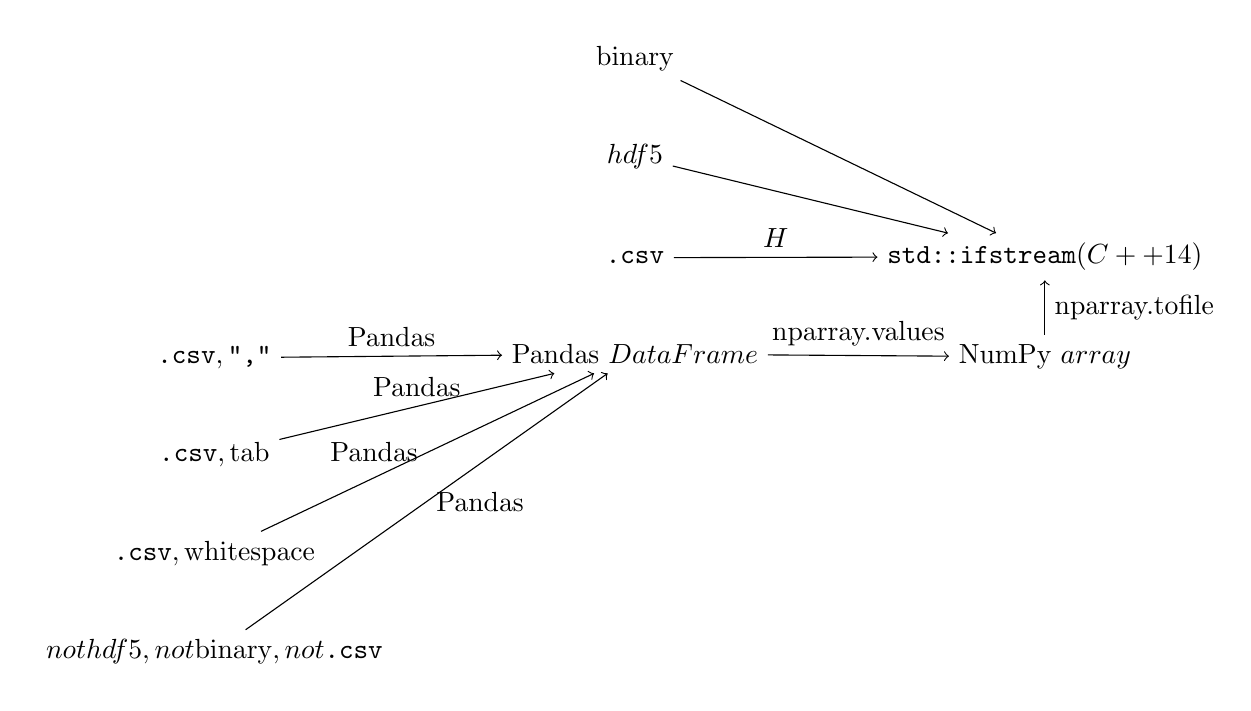
\begin{tikzpicture}
\matrix (m) [matrix of math nodes, row sep=2em, column sep=4em, minimum width=1.75em]
{
	& \text{binary} &   \\
	& hdf5   & 	\\
%	& \verb|.csv| & \boxed{ \verb|std::ifstream| (C++14)  } \\
	& \verb|.csv| &   \verb|std::ifstream| (C++14)   \\
	\verb|.csv|, \verb|","|  &  \text{Pandas } DataFrame & \text{NumPy }  array \\
	\verb|.csv|, \text{tab}  &   & \\
	\verb|.csv|, \text{whitespace}  &  &  \\	
	not hdf5, not \text{binary}, not \verb|.csv|  &   & \\
};
\path[->]
(m-1-2) edge node [above] {$$} (m-3-3)
(m-2-2) edge node [above] {$$} (m-3-3)
(m-3-2) edge node [above] {$H$} (m-3-3)
(m-4-1) edge node [above] {Pandas} (m-4-2)
(m-4-2) edge node [above] { nparray.values } (m-4-3)
(m-5-1) edge node [above] {Pandas} (m-4-2)
(m-6-1) edge node [left] {Pandas} (m-4-2)
(m-7-1) edge node [right] {Pandas} (m-4-2)
(m-4-3) edge node [right] { nparray.tofile } (m-3-3)
;
\end{tikzpicture}
\end{equation}



\part{Introduction}





\subsubsection{Terminology} \quad \\ 
inputs $\equiv $ independent variables $\equiv $ predictors (cf. statistics) $ \equiv $ features (cf. pattern recognition) \\
outputs $\equiv $ dependent variables $\equiv $ responses

cf. Chapter 2 Overview of Supervised Learning, Section 2.1 Introduction of Hastie, Tibshirani, and Friedman (2009) \cite{HTF2009}

cf. Chapter 2 Overview of Supervised Learning, Section 2.2 Variable Types and Terminology  of Hastie, Tibshirani, and Friedman (2009) \cite{HTF2009}

\subsubsection{$\text{FinSet}$} \quad \\ 
The category $\text{FinSet} \in \mathbf{\text{Cat}}$ is the category of all finite sets (i.e. $\text{Obj}(\text{FinSet}) \equiv $ all finite sets) and all functions in between them; note that $\text{FinSet} \subset \mathbf{\text{Set}}$ \footnote{nlab $\text{FinSet}$ \url{https://ncatlab.org/nlab/show/FinSet}}

Recall that the $\text{FinSet}$ \emph{skeletal} is


\subsection{Supervised Learning}

cf. \url{http://cs229.stanford.edu/notes/cs229-notes1.pdf}

Consider data to belong to the category of all possible data:
\[
\text{Data} \equiv \text{Dat} = (\text{Obj}(\text{Dat}), \text{Mor}\text{Dat}, 1, \circ), \qquad \, \text{Dat} \in \mathbf{\text{Cat}}
\]
Consider the \textbf{training set}:
\[
\text{training set} := \lbrace (x^{(i)},y^{(i)}) | i  =1 \dots m , x^{(i)} \in \mathcal{X}, y^{(i)} \in \mathcal{Y} \rbrace
\]
where $\mathcal{X}$ is a manifold (it can be topological or smooth, EY:20160502 I don't know exactly because I need to check the topological and/or differential structure); $\mathcal{Y} \in \text{Obj}(\text{FinSet})$, or $(\mathcal{Y} \in \text{Obj}(\text{Top}) (\text{or } \mathcal{Y} \in \text{Obj}(\text{Man})))$.  

So training set $ \subset \mathcal{X} \times \mathcal{Y} \in \text{Obj}(\text{Dat})$.  

I propose that there should be a functor $H$ that represents the ``learning algorithm'':
\[
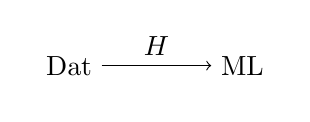
\begin{tikzpicture}
  \matrix (m) [matrix of math nodes, row sep=3em, column sep=4em, minimum width=2em]
  {
\text{Dat} & \text{ML}  \\
};
  \path[->]
  (m-1-1) edge node [above] {$H$} (m-1-2)
  ;
\end{tikzpicture}
\]
s.t.
\[
\begin{aligned}
  & H:\mathcal{X}\times \mathcal{Y} \to \text{Hom}(\mathcal{X}, \mathcal{Y}) \\ 
  & H(\text{training set}) = H(\lbrace (x^{(i)},y^{(i)} )| i  =1 \dots m \rbrace) = h 
\end{aligned}
\]

When $\mathcal{Y} \in \text{Obj}(\text{FinSet})$, \emph{classification}. \\
When $\mathcal{Y} \in \text{Obj}(\text{Top})$ (or $\text{Obj}(\text{Man})$, \emph{regression}.

\subsubsection{Linear Regression}

Keeping in mind   
\[
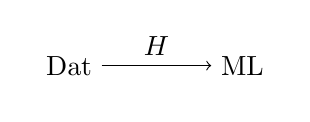
\begin{tikzpicture}
  \matrix (m) [matrix of math nodes, row sep=3em, column sep=4em, minimum width=2em]
  {
\text{Dat} & \text{ML}  \\
};
  \path[->]
  (m-1-1) edge node [above] {$H$} (m-1-2)
  ;
\end{tikzpicture}
\]
Consider \[
\begin{aligned}
  & h:\mathbb{R}^p \to \text{Hom}(\mathcal{X},\mathcal{Y}) \\ 
  & h:\theta \mapsto h_{\theta} 
\end{aligned}
\]
s.t. 
\[
h_{\theta} : \mathcal{X} \to \mathcal{Y}
\]
so (possibly) $h\in \text{Obj}ML$ (or is $h$ part of the functor $H$?)

Consider the cost function $J$
\[
\begin{aligned}
  & J:\mathbb{R}^p \to \text{Hom}(\mathfrak{X}\times \mathfrak{Y}, \mathbb{R}) = C^{\infty}(\mathcal{X}\times \mathcal{Y}) \\ 
  & J(\theta) = \frac{1}{2} \sum_{i=1}^m (h_{\theta}(x^{(i)}) - y^{(i)})^2 
\end{aligned}
\]

\subsubsection{LMS algorithm (least mean square (or Widrow-Hoff learning rule))}

Define \textbf{gradient descent} algorithm:
\[
\theta_j := \theta_j- \alpha \frac{ \partial }{ \partial \theta_j} J(\theta)
\]
with $:=$ being assignment (I'll use $:=$ for ``define'', in mathematical terms, use context to distinguish the 2), where $\alpha$ is the \emph{learning rate}.  

Rewriting the above,
\[
\theta := \theta - \alpha \text{grad}J(\theta)
\]
where $\text{grad} : C^{\infty}(M) \to \mathfrak{X}(M)$, with $M$ being a smooth manifold.  

This is \emph{batch gradient descent}:
\[
\begin{gathered}
  \theta_j := \theta_j -\alpha \frac{ \partial }{ \partial \theta_j} J(\theta) = \theta_j - \alpha \frac{ \partial }{ \partial \theta_j} \frac{1}{2} \sum_{i=1}^m ( h_{\theta}(x^{(i)}) - y^{(i)})^2  = \theta_j - \alpha \sum_{i=1}^m (h_{\theta}(x^{(i)}) - y^{(i)} ) \left( \frac{ \partial h_{\theta}(x^{(i)}) }{\partial \theta} \right)
\end{gathered}
\]
Simply notice how the entire training set of $m$ rows is used.  

I will expound on the so-called distinguished object $1\xrightarrow{P}X$ on pp. 8, in Section 2 The Category of Conditional Probabilities of Culbertson and Sturtz (2013) \cite{CS2013} because it wasn't clear to me in the first place (the fault is mine; the authors wrote a very lucid and very fathomable, pedagogically-friendly exposition).  

$\forall \, Y $ with indiscrete $\sigma$-algebra $\Sigma_Y = \lbrace Y ,\emptyset \rbrace$ \\
\phantom{ \qquad \, } (remember, $((Y,\Sigma_Y), \mu_Y)$, $\mu_Y(\phi) = 0$, $\mu_Y(Y)=1$), \\
\qquad \\ 
$\exists \, !$ unique morphism in $\text{Mor}\mathcal{P}$, $X\to Y$, since 

$\forall \, P:X\to Y$, $P \in \text{Mor}\mathcal{P}$, $P_x$ must be a probability measure on $Y$, because 
\[
\begin{gathered}
  (X,\Sigma_X) \xrightarrow{ P } (Y,\Sigma_Y) \\ 
  P:\Sigma_Y\times X \to [0,1] \\ 
  P(\cdot | x):\Sigma_Y \to [0,1] \equiv \begin{gathered} P_x:\Sigma_Y \to [0,1]  \text{ s.t. }  \\ P_x(\emptyset) =0, \, P_x(Y) =1 \end{gathered}
\end{gathered}
\]
i.e. EY: 20160503, Given $x\in X$ occurs, $Y$ must occur. 

By def. of terminal object ($\forall \, (X,\Sigma_X) \in \text{Obj}\mathcal{P}$, $\exists \, !$ morphism $P$ s.t. $(X,\Sigma_X) \xrightarrow{P} (Y,\Sigma_Y)$, \\
$Y$ \emph{terminal} object, and denote unique morphism $!_X : X\to Y$, $!_X \in \text{Mor}\mathcal{P}$.  

Up to isomorphism, canonical terminal object is 1-element set denoted by $1 = \lbrace * \rbrace$, with the only possible $\sigma$-algebra ($\mu(*)=1, \, \mu(\emptyset) = 0$),

\[
\forall \, P:1 \to X, \, P\in \text{Mor}\mathcal{P}, \, P \in \text{Hom}_{\mathcal{P}}(1,X) , \, \forall \, X \in \text{Mor}\mathcal{P}
\]
$P$ is an ``absolute'' probability measure on $X$ because ``there's no variability (conditioning) possible within singleton set $1 = \lbrace * \rbrace$.''  \cite{CS2013}

Now
\[
\begin{aligned}
  & P:\Sigma_X \times 1 \to [0,1] \\ 
  & P(\cdot | *) : \Sigma_X \to [0,1]
\end{aligned}
\]
where $P(\cdot | *) : \Sigma_X \to [0,1]$ perfect probability measure on $X$, $P(\cdot | *) : \Sigma_X \to [0,1] \equiv P_*$, i.e. $P(\cdot | *) = p(\cdot )$ (usual probability on $X$).  

$\forall \, A \in \Sigma_X$, $P(A|\cdot ) : 1 \to [ 0,1]$, but $P(A|*) = P(A)$, $P(A|\emptyset ) = 0$.  

Refer to 
\[
1\xrightarrow{P} X
\]
morphism $P:1\to X \in \text{Mor}\mathcal{P}$ as probability measure or distribution on $X$.  



\section{Deep Learning}

Deep Learning Tutorial \cite{LISA2015}




\section{Parallel Computing}

\subsection{Udacity Intro to Parallel Programming : Lesson 1 - The GPU Programming Model}

Owens and Luebki pound fists at the end of this video.  $=))))$  \href{https://classroom.udacity.com/courses/cs344/lessons/55120467/concepts/658304810923}{Intro to the class}.

\subsubsection{Running CUDA locally}
Also, \href{https://classroom.udacity.com/courses/cs344/lessons/55120467/concepts/658304810923}{Intro to the class}, in Lesson 1 - The GPU Programming Model, has links to documentation for running CUDA locally; in particular, for Linux: \url{http://docs.nvidia.com/cuda/cuda-getting-started-guide-for-linux/index.html}.  That guide told me to go download the NVIDIA CUDA Toolkit, which is the \href{NVIDIA CUDA Developer Toolkit}{https://developer.nvidia.com/cuda-downloads}.  

For \emph{Fedora}, I chose Installer Type \verb|runfile (local)|.  

Afterwards, installation of CUDA on Fedora 23 workstation had been nontrivial.  Go see either my github repository \href{https://github.com/ernestyalumni/MLgrabbag/blob/master/README.md}{MLgrabbag} (which will be updated) or my \href{https://ernestyalumni.wordpress.com/2016/05/07/fedora-23-workstation-linuxnvidia-geforce-gtx-980-ti-my-experience-log-of-what-i-do-and-find-out/#CUDAinstall}{wordpress blog} (which may not be upgraded frequently).  


$P=VI = I^2R$ heating.

\subsubsection{Definitions of Latency and throughput (or bandwidth)}

cf. 
\href{https://classroom.udacity.com/courses/cs344/lessons/55120467/concepts/669874580923}{Building a Power Efficient Processor}

\href{https://classroom.udacity.com/courses/cs344/lessons/55120467/concepts/667559300923}{Latency vs Bandwidth}

latency $[\text{sec}]$.  From the title ``Latency vs. bandwidth'', I'm thinking that throughput $=$ bandwidth (???).  throughput $ = $ job$/$time (of job).  

Given total task, velocity $v$, \\
total task $/v = $ latency.  throughput $=$ latency$/(\text{jobs per total task})$.  


Also, in \href{https://classroom.udacity.com/courses/cs344/lessons/55120467/concepts/669874580923}{Building a Power Efficient Processor}.  Owens recommends the article David Patterson, ``Latency...''

cf. \href{https://classroom.udacity.com/courses/cs344/lessons/55120467/concepts/671181630923}{GPU from the Point of View of the Developer}

$n_{\text{core}} \equiv $ number of cores \\
$n_{\text{vecop}} \equiv$ ($n_{\text{vecop}}-$wide axial vector operations$/core$ core) \\
$n_{\text{thread}} \equiv $ threads$/$core (hyperthreading)
\[
n_{\text{core}} \cdot n_{\text{vecop}} \cdot n_{\text{thread}}  \text{ parallelism  }
\]

There were various websites that I looked up to try to find out the capabilities of my video card, but so far, I've only found these commands (and I'll print out the resulting output):
{\scriptsize
\begin{lstlisting}
$ lspci -vnn | grep VGA -A 12
03:00.0 VGA compatible controller [0300]: NVIDIA Corporation GM200 [GeForce GTX 980 Ti] [10de:17c8] (rev a1) (prog-if 00 [VGA controller])
	Subsystem: eVga.com. Corp. Device [3842:3994]
	Physical Slot: 4
	Flags: bus master, fast devsel, latency 0, IRQ 50
	Memory at fa000000 (32-bit, non-prefetchable) [size=16M]
	Memory at e0000000 (64-bit, prefetchable) [size=256M]
	Memory at f0000000 (64-bit, prefetchable) [size=32M]
	I/O ports at e000 [size=128]
	[virtual] Expansion ROM at fb000000 [disabled] [size=512K]
	Capabilities: <access denied>
	Kernel driver in use: nvidia
	Kernel modules: nouveau, nvidia

$ lspci | grep VGA -E
03:00.0 VGA compatible controller: NVIDIA Corporation GM200 [GeForce GTX 980 Ti] (rev a1)

$ grep driver /var/log/Xorg.0.log
[    18.074] Kernel command line: BOOT_IMAGE=/vmlinuz-4.2.3-300.fc23.x86_64 root=/dev/mapper/fedora-root ro rd.lvm.lv=fedora/root rd.lvm.lv=fedora/swap rhgb quiet LANG=en_US.UTF-8 nouveau.modeset=0 rd.driver.blacklist=nouveau nomodeset gfxpayload=vga=normal
[    18.087] (WW) Hotplugging is on, devices using drivers 'kbd', 'mouse' or 'vmmouse' will be disabled.
[    18.087] 	X.Org XInput driver : 22.1
[    18.192] (II) Loading /usr/lib64/xorg/modules/drivers/nvidia_drv.so
[    19.088] (II) NVIDIA(GPU-0): Found DRM driver nvidia-drm (20150116)
[    19.102] (II) NVIDIA(0):     ACPI event daemon is available, the NVIDIA X driver will
[    19.174] (II) NVIDIA(0): [DRI2]   VDPAU driver: nvidia
[    19.284] 	ABI class: X.Org XInput driver, version 22.1
...

$ lspci -k | grep -A 8 VGA
03:00.0 VGA compatible controller: NVIDIA Corporation GM200 [GeForce GTX 980 Ti] (rev a1)
	Subsystem: eVga.com. Corp. Device 3994
	Kernel driver in use: nvidia
	Kernel modules: nouveau, nvidia
03:00.1 Audio device: NVIDIA Corporation GM200 High Definition Audio (rev a1)
	Subsystem: eVga.com. Corp. Device 3994
	Kernel driver in use: snd_hda_intel
	Kernel modules: snd_hda_intel
05:00.0 USB controller: VIA Technologies, Inc. VL805 USB 3.0 Host Controller (rev 01)
  \end{lstlisting}
}
\href{https://classroom.udacity.com/courses/cs344/lessons/55120467/concepts/671181640923}{CUDA Program Diagram}

\[
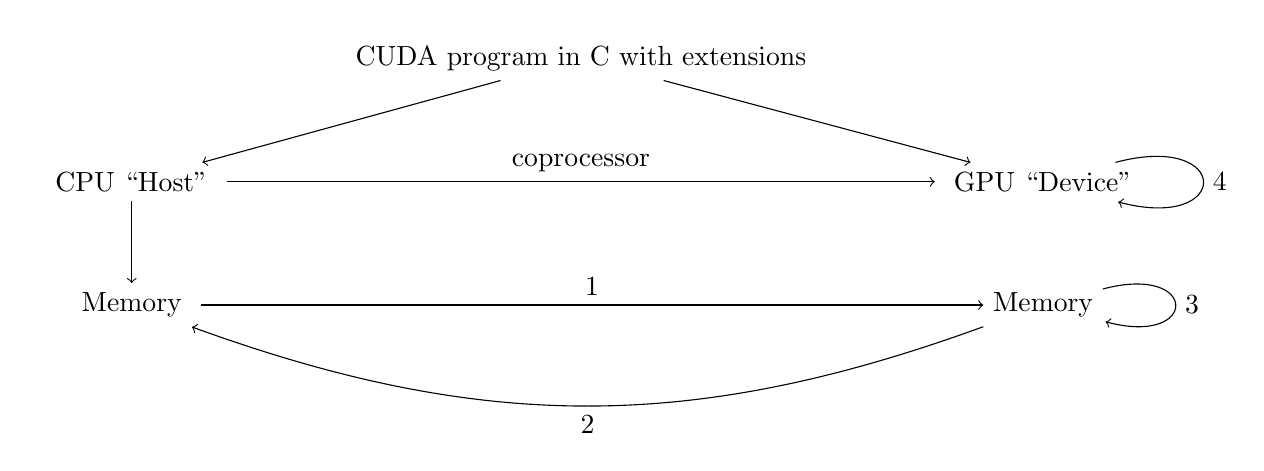
\begin{tikzpicture}
  \matrix (m) [matrix of math nodes, row sep=3em, column sep=4em, minimum width=1em]
  {
    & \text{ CUDA program in C with extensions } &  \\
    \text{ CPU ``Host'' } & & \text{ GPU ``Device'' } \\
    \text{ Memory } & & \text{Memory} \\
};
  \path[->]
  (m-1-2) edge node [above] {} (m-2-1)
  edge node [above] {} (m-2-3)
  (m-2-1) edge node [above] { coprocessor } (m-2-3)
  edge node [above] {} (m-3-1)
  (m-3-1) edge node [above] {$1$} (m-3-3)
  (m-3-3) edge [bend left=20] node [below] {$2$} (m-3-1)
  edge [loop right] node [right] {$3$} (m-3-3)
  (m-2-3) edge [loop right] node [right] {$4$} (m-2-3)
  ;
\end{tikzpicture}
\]
CPU ``host'' is the boss (and issues commands) -Owen.

$\text{Coprocessor} : \text{ CPU ``host'' } \to \text{ GPU ``device'' } $ \\
$\text{Coprocessor} : \text{ CPU process } \mapsto \text{ (co)-process out to GPU } $ \\

With
\begin{enumerate}
  \item[1] data cpu $\to $ gpu
  \item[2] data gpu $\to$ cpu \qquad (initiated by cpu host) \\

$1.,2.,$ uses \verb|cudaMemcpy| 
  \item[3] allocate GPU memory: \verb|cudaMalloc|
  \item[4] launch kernel on GPU
  \end{enumerate}
Remember that for 4., this launching of the kernel, while it's acting on GPU ``device'' onto itself, it's initiated by the boss, the CPU ``host''.

Hence, cf. \href{https://classroom.udacity.com/courses/cs344/lessons/55120467/concepts/670489380923}{Quiz: What Can GPU Do in CUDA}, GPUs can respond to CPU request to receive and send Data CPU $\to $ GPU and Data GPU $\to $ CPU, respectively (1,2, respectively), and compute a kernel launched by the CPU (3).


\href{https://classroom.udacity.com/courses/cs344/lessons/55120467/concepts/670742800923}{A CUDA Program}
A typical GPU program

\begin{itemize}
\item \verb|cudaMalloc| - CPU allocates storage on GPU 
\item \verb|cudaMemcpy| - CPU copies input data from CPU $\to $ GPU 
\item \emph{kernel launch} - CPU launches kernel(s) on GPU to process the data 
\item \verb|cudaMemcpy| - CPU copies results back to CPU from GPU
  \end{itemize}

Owens advises minimizing ``communication'' as much as possible (e.g. the \verb|cudaMemcpy| between CPU and GPU), and do a lot of computation in the CPU and GPU, each separately.

\href{https://classroom.udacity.com/courses/cs344/lessons/55120467/concepts/672300540923}{Defining the GPU Computation}

Owens circled this
{\Large
  \[
  \begin{gathered}
\text{ BIG IDEA } \qquad \, \boxed{ \text{ This is Important } }  \\
\begin{aligned} 
& \text{ Kernels look like serial programs } \\
  & \text{ Write your program as if it will run on \textbf{ one } thread } \\
  & \text{The GPU will run that program on \textbf{ many } threads}
  \end{aligned}
\end{gathered}
\]
}

\href{https://classroom.udacity.com/courses/cs344/lessons/55120467/concepts/670742840923}{Squaring A Number on the CPU}

Note
\begin{enumerate}
\item Only 1 thread of execution: (``thread'' $:=$ one independent path of execution through the code) e.g. the \verb|for| loop
  \item no explicit parallelism; it's serial code e.g. the \verb|for| loop through 64 elements in an array
  \end{enumerate}


\href{https://classroom.udacity.com/courses/cs344/lessons/55120467/concepts/670742870923}{GPU Code A High Level View}

CPU:
\begin{itemize}
  \item Allocate Memory 
  \item Copy Data to/from GPU
    \item Launch Kernel - species degree of parallelism
\end{itemize}

GPU:
\begin{itemize}
\item Express Out $=$ In $\cdot $ In  - says \emph{nothing} about the degree of parallelism
  \end{itemize}

Owens reiterates that in the GPU, everything looks serial, but it's only in the CPU that anything parallel is specified.  

pseudocode: CPU code: square kernel $<<< 64 >>>$ (outArray,inArray)

\href{https://classroom.udacity.com/courses/cs344/lessons/55120467/concepts/670742940923}{Squaring Numbers Using CUDA Part 3}

From the example
\begin{lstlisting}
  // launch the kernel
  square<<<1, ARRAY_SIZE>>>(d_out, d_in)
  \end{lstlisting}
we're introduced to the ``CUDA launch operator'', initiating a kernel of 1 block of 64 elements (\verb|ARRAY_SIZE| is 64) on the GPU.  Remember that \verb|d_| prefix (this is naming comvention) tells us it's on the device, the GPU, solely.  

With CUDA launch operator $\equiv <<<>>>$, then also looking at this explanation on \verb|stackexchange| (so surely others are confused as well, of those who are learning this (cf. \href{http://stackoverflow.com/questions/19240658/cuda-kernel-launch-parameters-explained-right}{CUDA kernel launch parameters explained right?}).  From \href{http://stackoverflow.com/users/1957265/eric}{Eric}'s answer, \\

threads are grouped into blocks.  all the threads will execute the invoked kernel function.

Certainly,
\[
\begin{aligned}
  & <<<>>>:(n_{\text{block}}, n_{\text{threads}})\times \text{kernelfunctions} \mapsto \text{kernelfunction}<<<n_{\text{block}},n_{\text{threads}}>>> \in \text{End}:\text{Dat}_{\text{GPU}} \\ 
  & <<<>>>: \mathbb{N}^+ \times \mathbb{N}^+ \times \text{Mor}_{\text{GPU}} \to \text{End}\text{Dat}_{\text{GPU}}
  \end{aligned}
\]
where I propose that GPU can be modeled as a category containing objects $\text{Dat}_{\text{GPU}}$, the collection of all possible data inputs and outputs into the GPU, and $\text{Mor}_{\text{GPU}}$, the collection of all kernel functions that run (exclusively, and this \emph{must} be the class, as reiterated by Prof. Owen) on the GPU.

Next,
\[
\begin{aligned}
  & \text{kernelfunction}<<<n_{\text{block}},n_{\text{threads}}>>>: \text{din}\mapsto \text{dout} \qquad \, (\text{as given in the ``square'' example, and so I propose}) \\ 
  & \text{kernelfunction}<<<n_{\text{block}},n_{\text{threads}}>>>:(\mathbb{N}^+)^{n_{\text{threads}}} \to (\mathbb{N}^+)^{n_{\text{threads}}}
  \end{aligned}
\]
But keep in mind that $\text{dout}$, $\text{din}$ are pointers in the C program, pointers to the place in the memory.  

\verb|cudaMemcopy| is a functor category, s.t. e.g. $\text{Obj}_{\text{CudaMemcopy}} \ni \text{cudaMemcpyDevicetoHost}$ where
\[
\text{cudaMemcopy}(-,-,n_{\text{thread}},\text{cudaMemcpyDeviceToHost}): \text{Memory}_{\text{GPU}} \to \text{Memory}_{\text{CPU}} \in \text{Hom}(\text{Memory}_{\text{GPU}}, \text{Memory}_{\text{CPU}})
\]

\href{https://classroom.udacity.com/courses/cs344/lessons/55120467/concepts/670742910923}{Squaring Numbers Using CUDA 4}

Note the C language construct \emph{declaration specifier} - denotes that this is a kernel (for the GPU) and not CPU code.  Pointers need to be allocated on the GPU (otherwise your program will crash spectacularly -Prof. Owen).  

\subsubsection{What are C pointers?}

Is $\langle \text{ type } \rangle \, *$, a pointer, then a mapping from the category, namely the objects of types, to a mapping from the specified value type to a memory address?

e.g.
\[
\begin{aligned}
  \langle \, \rangle \, * & : \text{float} \mapsto \text{float} \, * \\ 
  \text{float } \, * & : \text{din} \mapsto \text{ some memory address }
\end{aligned}
\]
and then we pass in mappings, not values, and so we're actually declaring a square \emph{functor}.

What is \verb|threadIdx|?  What is it mathematically?  Consider that $\exists \,$ 3 ``modules'':

\[
\begin{aligned}
  & \text{threadIdx}.x \\
  & \text{threadIdx}.y \\
  & \text{threadIdx}.z 
\end{aligned}
\]
And then the line
\begin{lstlisting}
int idx = threadIdx.x;
  \end{lstlisting}
says that idx is an integer, ``declares'' it to be so, and then assigns idx to $\text{threadIdx}.x$ which surely has to also have the same type, integer.  So (perhaps)
\[
idx \equiv \text{threadIdx}.x \in \mathbb{Z}
\]
is the same thing.

Then suppose threadIdx $\subset \mathbf{\text{FinSet}}$, a subcategory of the category of all (possible) finite sets, s.t. threadIdx has 3 particular morphisms, $x,y,z\in \text{Mor}threadIdx$,
\[
\begin{aligned}
  & x : \text{threadIdx} \mapsto \text{threadIdx}.x \in \text{Obj}_{\mathbf{\text{FinSet}}} \\ 
  & y : \text{threadIdx} \mapsto \text{threadIdx}.x \in \text{Obj}_{\mathbf{\text{FinSet}}} \\ 
  & z : \text{threadIdx} \mapsto \text{threadIdx}.x \in \text{Obj}_{\mathbf{\text{FinSet}}}  
\end{aligned}
\]

\href{https://classroom.udacity.com/courses/cs344/lessons/55120467/concepts/670742980923}{Configuring the Kernel Launch Parameters Part 1}

$n_{\text{blocks}}$, $n_{\text{threads}}$ with $n_{\text{threads}} \geq 1024$ (this maximum constant is GPU dependent).  You should pick the $(n_{\text{blocks}}, n_{\text{threads}})$ that makes sense for your problem, says Prof. Owen.  

\subsubsection{Memory layout of blocks and threads}

$\forall \, (n_{\text{blocks}}, n_{\text{threads}}) \in \mathbb{Z} \times \lbrace 1 \dots 1024 \rbrace$, $\lbrace 1 \dots n_{\text{block}} \times \lbrace 1 \dots n_{\text{threads}} \rbrace$ is now an ordered index (with lexicographical ordering).  This is just 1-dimensional (so possibly there's a 1-to-1 mapping to a finite subset of $\mathbb{Z}$).

I propose that ``adding another dimension'' or the 2-dimension, that Prof. Owen mentions is being able to do the Cartesian product, up to 3 Cartesian products, of the block-thread index.  

\href{https://classroom.udacity.com/courses/cs344/lessons/55120467/concepts/668398860923}{Quiz: Configuring the Kernel Launch Parameters 2 }

Most general syntax:

Configuring the kernel launch
\begin{lstlisting}
  kernel<<<grid of blocks, block of threads >>>(...)

  // for example

  square<<<dim3(bx,by,bz), dim3(tx,ty,tz), shmem>>>(...)
  \end{lstlisting}
where \verb|dim3(tx,ty,tz)| is the grid of blocks $bx\cdot by \cdot bz$ \\
\phantom{ where } \verb|{dim3}(tx,ty,tz)| is the block of threads $tx \cdot ty \cdot tz$ \\
\phantom{ where } \verb|shmem| is the shared memory per block in bytes


\href{https://classroom.udacity.com/courses/cs344/lessons/55120467/concepts/967066740923}{Problem Set 1}
``Also, the image is represented as an 1D array in the kernel, not a 2D array like I mentioned in the video.''

Here's part of that code for squaring numbers:
\begin{lstlisting}
  __global__ void square(float *d_out, float *d_in) {
    int idx = threadIdx.x;
    float f = d_in[idx];
    d_out[idx] = f*f;
    }
  \end{lstlisting}

\subsubsection{Grid of blocks, block of threads, thread that's indexed; (mathematical) structure of it all}

Let
\[
\begin{gathered}
  \text{grid} = \prod_{I=1}^N (\text{block})^{n_I^{\text{block}}}
\end{gathered}
\]
where $N=1,2,3$ (for CUDA) and by naming convention $\begin{aligned} & \quad \\
  & I = 1 \equiv x \\
  & I = 2 \equiv y \\
  & I = 3 \equiv z \end{aligned}$

Let's try to make it explicity (as others had difficulty understanding the grid, block, thread model, cf. \href{http://stackoverflow.com/questions/14711668/colored-image-to-greyscale-image-using-cuda-parallel-processing}{colored image to greyscale image using CUDA parallel processing}, \href{http://stackoverflow.com/questions/16619274/cuda-griddim-and-blockdim}{Cuda gridDim and blockDim}) through commutative diagrams and categories (from math):

\[
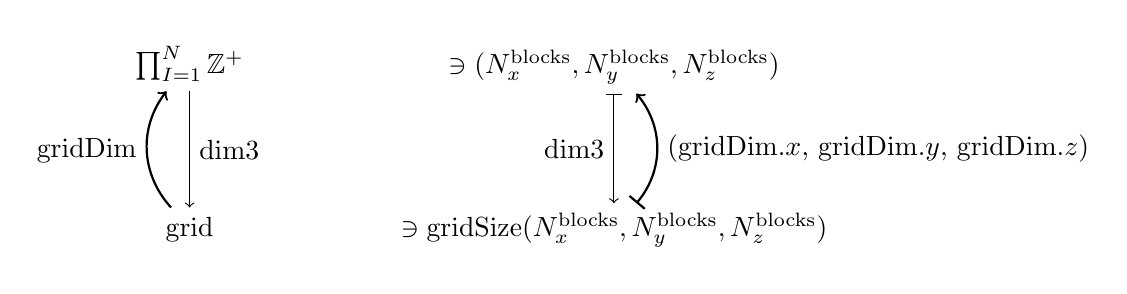
\begin{tikzpicture}
  \matrix (m) [matrix of math nodes, row sep=4em, column sep=5em, minimum width=2em]
  {
\prod_{I=1}^N \mathbb{Z}^+ & \ni (N_x^{\text{blocks}}, N_y^{\text{blocks}} , N_z^{\text{blocks}}) \\
\text{grid} & \ni \text{gridSize}(N_x^{\text{blocks}}, N_y^{\text{blocks}} , N_z^{\text{blocks}} ) \\
};
  \path[->]
  (m-1-1) edge node [right] {$\text{dim}3$} (m-2-1)
  (m-2-1) edge [bend left=40, thick] node [left] {$\text{gridDim}$} (m-1-1)
  ;
  \path[|->]
  (m-1-2) edge node [left] {$\text{dim}3$} (m-2-2)
  (m-2-2) edge [bend right=40, thick] node [right] {$(\text{gridDim}.x$, $\text{gridDim}.y$, $\text{gridDim}.z)$} (m-1-2)
  ;  
\end{tikzpicture}
\]

\[
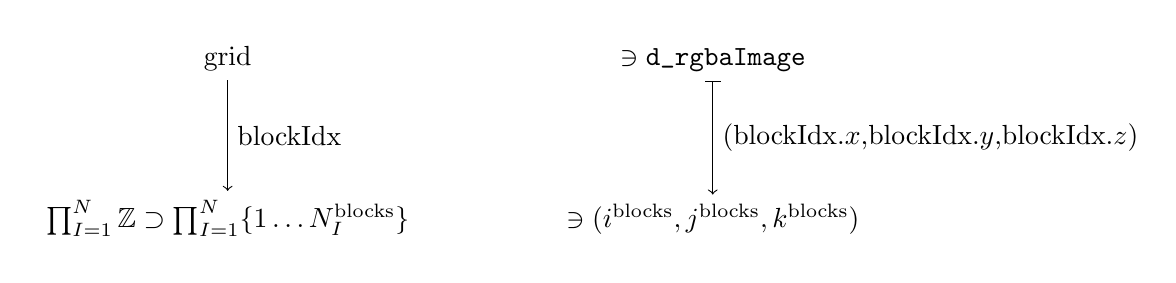
\begin{tikzpicture}
  \matrix (m) [matrix of math nodes, row sep=4em, column sep=5em, minimum width=2em]
  {
    \text{grid} & \ni \verb|d_rgbaImage| \\
    \prod_{I=1}^N \mathbb{Z} \supset \prod_{I=1}^N \lbrace 1 \dots N_I^{\text{blocks}} \rbrace & \ni (i^{\text{blocks}},j^{\text{blocks}}, k^{\text{blocks}} ) \\
};
  \path[->]
  (m-1-1) edge node [right] {$\text{blockIdx}$} (m-2-1)
  ;
  \path[|->]
  (m-1-2) edge node [right] {($\text{blockIdx}.x$,$\text{blockIdx}.y$,$\text{blockIdx}.z$)} (m-2-2)
  ;
  \end{tikzpicture}
\]

and then similar relations (i.e. arrows, i.e. relations) go for a block of threads:

\[
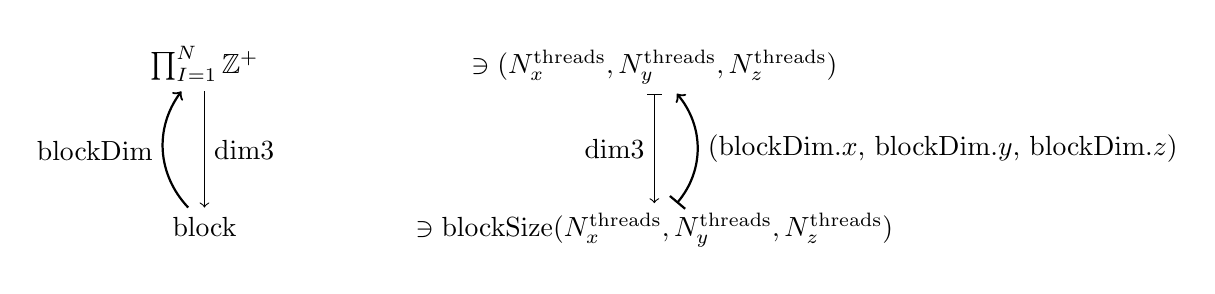
\begin{tikzpicture}
  \matrix (m) [matrix of math nodes, row sep=4em, column sep=5em, minimum width=2em]
  {
\prod_{I=1}^N \mathbb{Z}^+ & \ni (N_x^{\text{threads}}, N_y^{\text{threads}} , N_z^{\text{threads}}) \\
\text{block} & \ni \text{blockSize}(N_x^{\text{threads}}, N_y^{\text{threads}} , N_z^{\text{threads}} ) \\
};
  \path[->]
  (m-1-1) edge node [right] {$\text{dim}3$} (m-2-1)
  (m-2-1) edge [bend left=40, thick] node [left] {$\text{blockDim}$} (m-1-1)
  ;
  \path[|->]
  (m-1-2) edge node [left] {$\text{dim}3$} (m-2-2)
  (m-2-2) edge [bend right=40, thick] node [right] {$(\text{blockDim}.x$, $\text{blockDim}.y$, $\text{blockDim}.z)$} (m-1-2)
  ;  
\end{tikzpicture}
\]

\[
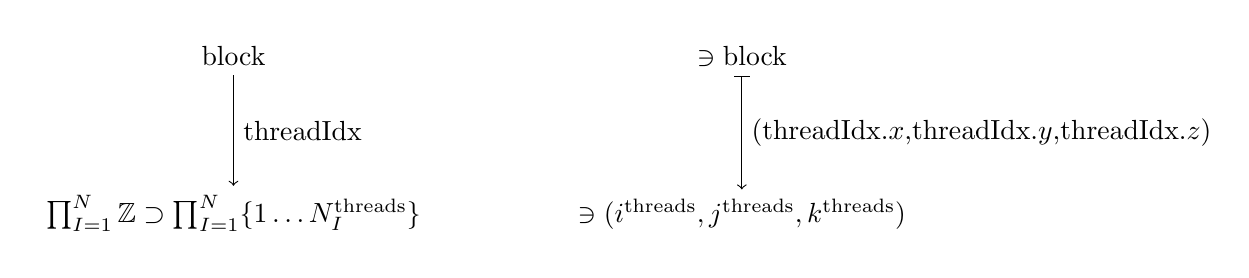
\begin{tikzpicture}
  \matrix (m) [matrix of math nodes, row sep=4em, column sep=5em, minimum width=2em]
  {
    \mathbf{\text{block}} & \ni \text{block} \\
    \prod_{I=1}^N \mathbb{Z} \supset \prod_{I=1}^N \lbrace 1 \dots N_I^{\text{threads}} \rbrace & \ni (i^{\text{threads}},j^{\text{threads}}, k^{\text{threads}} ) \\
};
  \path[->]
  (m-1-1) edge node [right] {$\text{threadIdx}$} (m-2-1)
  ;
  \path[|->]
  (m-1-2) edge node [right] {($\text{threadIdx}.x$,$\text{threadIdx}.y$,$\text{threadIdx}.z$)} (m-2-2)
  ;
  \end{tikzpicture}
\]

\href{https://discussions.udacity.com/t/gridsize-help-assignment-1-pp/124701}{gridsize help assignment 1 Pp} explains how threads per block is variable, and remember how Owens said Luebki says that a GPU doesn't get up for more than a 1000 threads per block.  

\subsubsection{Generalizing the model of an image}

Consider vector space $V$, e.g. $\text{dim}V=4$, vector space $V$ over field $\mathbb{K}$, so $V= \mathbb{K}^{\text{dim}V}$.

Each pixel represented by $\forall \, v \in V$.

Consider an image, or space, $M$.  $\text{dim}M = 2$ (image), $\text{dim}M=3$.  Consider a local chart (that happens to be global in our case):
\[
\begin{aligned}
  & \varphi : M \to \mathbb{Z}^{\text{dim}M} \supset \lbrace 1 \dots N_1 \rbrace \times \lbrace 1 \dots N_2 \rbrace \times \dots \times \lbrace 1 \dots N_{\text{dim}M} \rbrace \\ 
  & \varphi : x \mapsto (x^1(x), x^2(x), \dots , x^{\text{dim}M}(x) )
  \end{aligned}
\]
\[
\begin{tikzpicture}
  \matrix (m) [matrix of math nodes, row sep=4em, column sep=5em, minimum width=2em]
  {
    E & M \times V \\ 
    M &  \\
};
  \path[->]
  (m-1-1) edge node [auto] {$\varphi$} (m-1-2)
          edge node [left] {$\pi$} (m-2-1)
  (m-1-2) edge node [auto] {$$} (m-2-1)
              ;
  \end{tikzpicture}
\qquad \, 
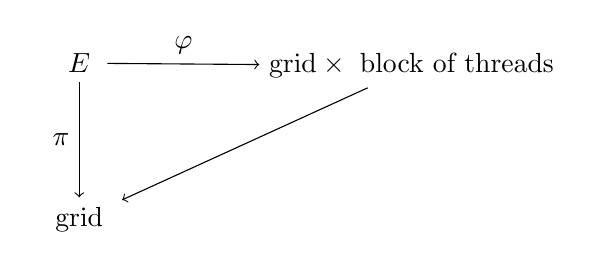
\begin{tikzpicture}
  \matrix (m) [matrix of math nodes, row sep=4em, column sep=5em, minimum width=2em]
  {
    E & \text{grid} \times \text{ block of threads } \\ 
    \text{ grid } & \\
};
  \path[->]
  (m-1-1) edge node [auto] {$\varphi$} (m-1-2)
          edge node [left] {$\pi$} (m-2-1)
  (m-1-2) edge node [auto] {$$} (m-2-1)
              ;
  \end{tikzpicture}
\]

Consider a ``coarsing'' of underlying $M$:
\[
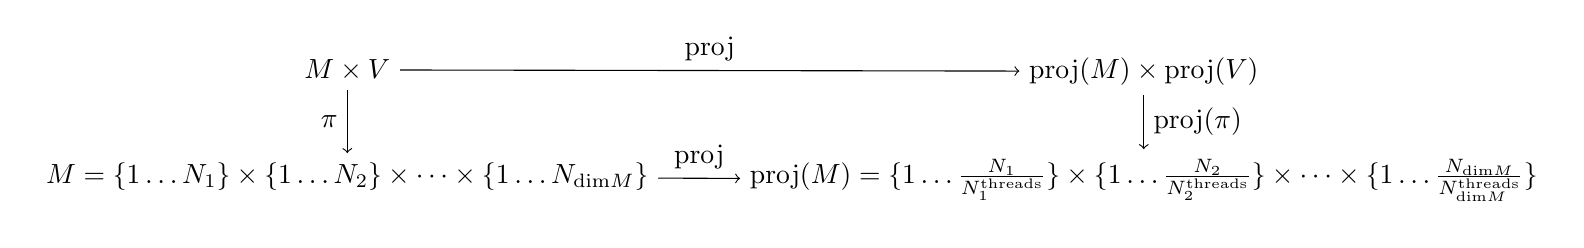
\begin{tikzpicture}
  \matrix (m) [matrix of math nodes, row sep=2em, column sep=3em, minimum width=1em]
  {
    M\times V & \text{proj}(M) \times \text{proj}(V) \\ 
    M = \lbrace 1 \dots N_1 \rbrace \times \lbrace 1 \dots N_2 \rbrace \times \dots \times \lbrace 1 \dots N_{\text{dim}M} \rbrace  & \text{proj}(M)  = \lbrace 1 \dots \frac{N_1}{N_1^{\text{threads}} } \rbrace \times \lbrace 1 \dots \frac{N_2}{N_2^{\text{threads}} } \rbrace \times \dots \times \lbrace 1 \dots \frac{N_{\text{dim}M}}{N_{\text{dim}M}^{\text{threads}} } \rbrace \\  
};
  \path[->]
  (m-1-1) edge node [auto] {$\text{proj}$} (m-1-2)
          edge node [left] {$\pi$} (m-2-1)
  (m-1-2) edge node [auto] {$\text{proj}(\pi)$} (m-2-2)
  (m-2-1) edge node [auto] {$\text{proj}$} (m-2-2)        
          ;
  \end{tikzpicture}
\]
e.g. $\begin{aligned} & \quad \\
  & N_1^{\text{thread}} = 12 \\
  & N_2^{\text{thread}} = 12 \end{aligned}$

Just note that in terms of syntax, you have the ``block'' model, in which you allocate blocks along each dimension.  So in
\[
\begin{aligned}
  & const \; dim3 \; blockSize(n^b_x, n^b_y, n^b_z) \\
  & const \; dim3 \; gridSize(n^{\text{gr}}_x, n^{\text{gr}}_y, n^{\text{gr}}_z)
  \end{aligned}
\]
Then the condition is
$n_x^b/\text{dim}V , n_y^b/\text{dim}V, n_z^b/\text{dim}V \in \mathbb{Z}$ (condition), \qquad \, $(n_x^{\text{gr}}-1)/\text{dim}V , n_y^{\text{gr}}/\text{dim}V, n_z^{\text{gr}}/\text{dim}V \in \mathbb{Z}$

\href{https://classroom.udacity.com/courses/cs344/lessons/77202674/concepts/773931440923}{Transpose Part 1}

Now
\[
\begin{gathered}
  \begin{aligned}
    & \text{Mat}_{\mathbb{F}}(n,n) \xrightarrow{T} \text{Mat}_{\mathbb{F}}(n,n) \\ 
    & A\mapsto A^T \text{ s.t. } (A^T)_{ij} = A_{ji}
    \end{aligned} \\ 
\begin{aligned}
  &  \text{Mat}_{\mathbb{F}} \xrightarrow{T} \mathbb{F}^{n^2} \\
  & A_{ij} \mapsto A_{ij} = A_{in + j }
  \end{aligned}
\end{gathered}
\]
\[
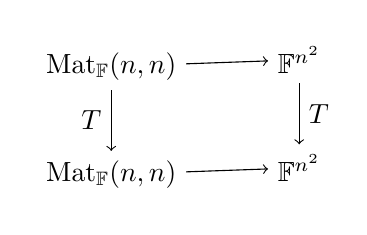
\begin{tikzpicture}
  \matrix (m) [matrix of math nodes, row sep=2em, column sep=3em, minimum width=1em]
  {
    \text{Mat}_{\mathbb{F}}(n,n) & \mathbb{F}^{n^2} \\
    \text{Mat}_{\mathbb{F}}(n,n) & \mathbb{F}^{n^2} \\ 
  };
  \path[->]
  (m-1-1) edge node [auto] {$$} (m-1-2)
          edge node [left] {$T$} (m-2-1)
  (m-1-2) edge node [auto] {$T$} (m-2-2)
  (m-2-1) edge node [auto] {$$} (m-2-2)        
          ;
  \end{tikzpicture} \qquad \, 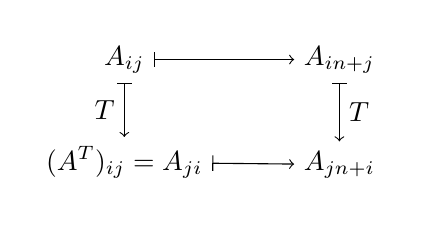
\begin{tikzpicture}
  \matrix (m) [matrix of math nodes, row sep=2em, column sep=3em, minimum width=1em]
  {
A_{ij} & A_{in+j} \\ 
(A^T)_{ij} = A_{ji} & A_{jn+i} \\
  };
  \path[|->]
  (m-1-1) edge node [auto] {$$} (m-1-2)
          edge node [left] {$T$} (m-2-1)
  (m-1-2) edge node [auto] {$T$} (m-2-2)
  (m-2-1) edge node [auto] {$$} (m-2-2)        
          ;
  \end{tikzpicture}
\]

\href{https://classroom.udacity.com/courses/cs344/lessons/77202674/concepts/773153710923}{Transpose Part 2}

Possibly, transpose is a functor.

Consider struct as a category.  In this special case, $\text{Obj}\text{struct} = \lbrace \text{arrays} \rbrace$ (a struct of arrays).  Now this struct already has a hash table for indexing upon declaration (i.e. ``creation''): so this category struct will need to be equipped with a ``diagram'' from the category of indices $J$ to struct: $J\to $ struct.

So possibly
\[
\begin{aligned}
  \text{struct} & \xrightarrow{T} & \text{ array } \\ 
 \text{Obj}\text{Struct} = \lbrace \text{ arrays } \rbrace & \xrightarrow{T} & \text{Obj}\text{array} = \lbrace \text{ struct } \rbrace \\ 
 J\to \text{ struct } & \xrightarrow{T} & J \to \text{ array } 
  \end{aligned}
\]







\href{https://classroom.udacity.com/courses/cs344/lessons/77202674/concepts/787012800923}{Quiz: What Kind Of Communication Pattern}
This quiz made a few points that clarified the characteristics of these so-called communication patterns (amongst the memory?)

\begin{itemize}
  \item map is bijective, and map $:\text{Idx} \to \text{Idx}$
  \item gather - not necessarily surjective
  \item scatter - not necessarily surjective 
  \item stencil - surjective
  \item transpose (see before)
  \end{itemize}




\href{https://classroom.udacity.com/courses/cs344/lessons/77202674/concepts/773153720923}{Parallel Communication Patterns Recap}

\begin{itemize}
\item map - bijective
\item transpose - bijective
\item gather - not necessarily surjective, and is many-to-one (by def.)
\item scatter - one-to-many (by def.) and is not necessarily surjective
\item stencil - several-to-one (not injective, by definition), and is surjective
\item reduce - all-to-one
  \item scan/sort - all-to-all
\end{itemize}

\href{https://classroom.udacity.com/courses/cs344/lessons/77202674/concepts/773153760923}{Programmer View of the GPU}

thread blocks: group of threads that cooperate to solve a (sub)problem

\href{https://classroom.udacity.com/courses/cs344/lessons/77202674/concepts/773153770923}{Thread Blocks And GPU Hardware}

CUDA GPU is a bunch of SMs:

Streaming Multiprocessors (SM)s

SMs have a bunch of simple processors and memory.

Dr. Luebki:
\[
\boxed{ \begin{gathered}
    \text{Let me say that again because it's really important} \\
    \text{GPU is responsible for allocating blocks to SMs}
  \end{gathered}
  }
\]
Programmer only gives GPU a pile of blocks.

\href{https://classroom.udacity.com/courses/cs344/lessons/77202674/concepts/787721730923}{Quiz: What Can The Programmer Specify}

I myself thought this was a revelation and was not intuitive at first:

Given a single kernel that's launched on many thread blocks include $X$, $Y$, the programmer cannot specify the sequence the blocks, e.g. block $X$, block $Y$, run (same time, or run one after the other), and which SM the block will run on (GPU does all this).  

\href{https://classroom.udacity.com/courses/cs344/lessons/77202674/concepts/787981160923}{Quiz: A Thread Block Programming Example}

Open up \verb|hello blockIdx.cu| in Lesson 2 Code Snippets (I got the repository from github, repo name is cs344).

At first, I thought you can do a single file compile and run in Eclipse without creating a new project.  No.  cf. \href{http://stackoverflow.com/questions/17164197/eclipse-creating-projects-every-time-to-run-a-single-file}{Eclipse creating projects every time to run a single file?}.  

%I opened it up in Eclipse with File, Open File (no need to create a new project).

I ended up creating a new CUDA C/C$++$ project from File -> New project, and then chose project type Executable, Empty Project, making sure to include Toolchain CUDA Toolkit (my version is 7.5), and chose an arbitrary project name (I chose cs344single).  Then, as suggested by \href{http://stackoverflow.com/users/3720356/kenny-nguyen}{Kenny Nguyen}, I dragged and dropped files into the folder, from my file directory program.

I ran the program with the ``Play'' triangle button, clicking on the green triangle button, and it ran as expected.  I also turned off Build Automatically by deselecting the option (no checkmark).

\href{https://classroom.udacity.com/courses/cs344/lessons/77202674/concepts/773883100923}{GPU Memory Model}

\[
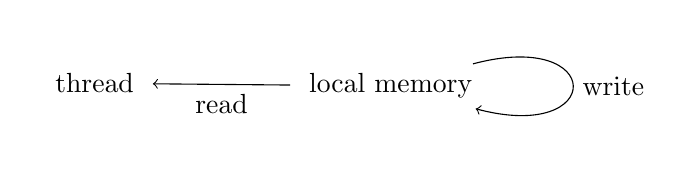
\begin{tikzpicture}
  \matrix (m) [matrix of math nodes, row sep=4em, column sep=5em, minimum width=2em]
  {
\text{ thread } & \text{ local memory } \\
};
  \path[->]
  (m-1-2) edge node [auto] {$\text{read}$} (m-1-1)
  (m-1-2) edge [loop right] node [right] {$\text{write}$} (m-1-2)
  ;
  \end{tikzpicture}
\]

Then consider threadblock $\equiv$  thread block \\
\phantom{Then consider } $\text{Obj}\text{threadblock} \supset \lbrace \text{ threads } \rbrace$ \\
\phantom{Then consider } $\text{FinSet} \xrightarrow{ \text{ threadIdx} } \text{ thread } \in \text{Mor}\text{threadblock}$

\[

\begin{tikzpicture}
  \matrix (m) [matrix of math nodes, row sep=4em, column sep=5em, minimum width=2em]
  {
\text{ threadblock } & \text{ shared memory } \\
};
  \path[->]
  (m-1-2) edge node [auto] {$\text{read}$} (m-1-1)
  (m-1-2) edge [loop right] node [right] {$\text{write}$} (m-1-2)
  ;
  \end{tikzpicture}
\]
$\forall \, $ thread,
\[
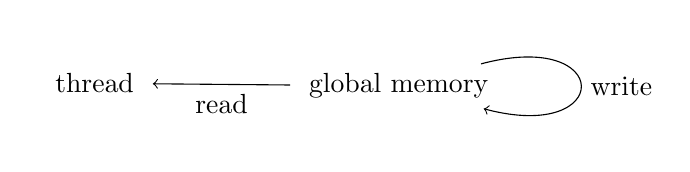
\begin{tikzpicture}
  \matrix (m) [matrix of math nodes, row sep=4em, column sep=5em, minimum width=2em]
  {
\text{ thread } & \text{ global memory } \\
};
  \path[->]
  (m-1-2) edge node [auto] {$\text{read}$} (m-1-1)
  (m-1-2) edge [loop right] node [right] {$\text{write}$} (m-1-2)
  ;
  \end{tikzpicture}
\]

\href{https://classroom.udacity.com/courses/cs344/lessons/77202674/concepts/773883130923}{Synchronization - Barrier}

\href{https://classroom.udacity.com/courses/cs344/lessons/77202674/concepts/785776150923}{Quiz: The Need For Barriers}

3 barriers were needed (wasn't obvious to me at first).  All threads need to finish the write, or initialization, so it'll need a barrier.

While
\begin{lstlisting}
array[idx] = array[idx+1];
  \end{lstlisting}
is 1 line, it'll actually need 2 barriers; first read.  Then write.

So \emph{actually} we'll need to \emph{rewrite} this code:
\begin{lstlisting}
  int temp = array[idx+1];
  __syncthreads();
  array[idx] = temp;
  __syncthreads();
  \end{lstlisting}

kernels have implicit barrier for each.  

\href{https://classroom.udacity.com/courses/cs344/lessons/77202674/concepts/774332060923}{Writing Efficient Programs}

\begin{enumerate}
\item Maximize \emph{arithmetic intensity}
  arithmetic intensity $:= \frac{ \text{ math } }{ \text{ memory }}$
  \end{enumerate}

\href{https://classroom.udacity.com/courses/cs344/lessons/77202674/concepts/774332070923}{video: Minimize Time Spent On Memory}

local memory is fastest; global memory is slower

\[
\text{local} > \text{ shared} >> \text{global} >> \text{CPU}
\]

kernel we know (in the code) is tagged with \verb|__global__|

\href{https://classroom.udacity.com/courses/cs344/lessons/77202674/concepts/814086830923}{quiz: A Quiz on Coalescing Memory Access}

Work it out as Dr. Luebki did to figure out if it's coalesced memory access or not.  


\href{https://classroom.udacity.com/courses/cs344/lessons/77202674/concepts/774332150923}{Atomic Memory Operations}

Atomic Memory Operations

atomicadd atomicmin atomicXOR atomicCAS Compare And Swap



\section{Pointers in C; Pointers in C categorified (interpreted in Category Theory)}

Suppose $v\in \text{ObjData}$, category of data \textbf{Data}, \\
\phantom{ Suppose} e.g. $v\in \text{Int} \in \text{Obj}\mathbf{\text{Type}}$, category of types $\mathbf{\text{Type}}$.

\[
\begin{aligned}
  & \text{Data}  \xrightarrow{ \& } \text{Memory}  \\
  & v \overset{\&}{\mapsto} \& v 
\end{aligned}
\]
with address $\& v \in $ Memory.

With \\
\phantom{With } assignment $pv = \& v$,
\[
\begin{aligned}
  & pv \in \text{Obj}\text{pointer}, \, \text{ category of pointers, pointer} \\ 
  & pv \in \text{Memory} \qquad \, (\text{i.e. not $pv \in \text{Dat}$, i.e. $pv \notin \text{Dat}$})
\end{aligned}
\]

\[
\text{ pointer } \ni pv \overset{ * }{ \mapsto } *pv \in \text{Dat}
\]

\[
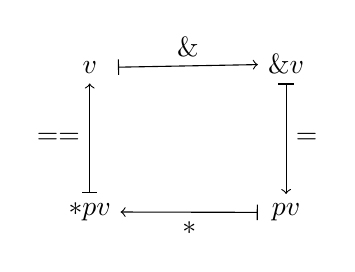
\begin{tikzpicture}
  \matrix (m) [matrix of math nodes, row sep=4em, column sep=5em, minimum width=2em]
  {
    v & \& v \\
    *pv & pv \\
};
  \path[|->]
  (m-1-1) edge node [auto] {$\&$} (m-1-2)
  (m-1-2) edge node [right] {$=$} (m-2-2)
  (m-2-2) edge node [auto] {$*$} (m-2-1)
  (m-2-1) edge node [left] {$==$} (m-1-1)
  ;
  \end{tikzpicture}
\qquad \, 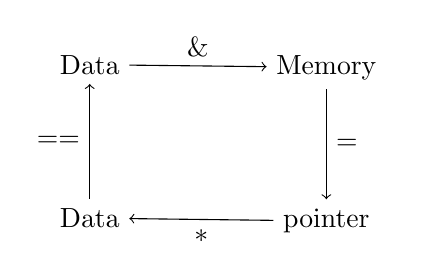
\begin{tikzpicture}
  \matrix (m) [matrix of math nodes, row sep=4em, column sep=5em, minimum width=2em]
  {
    \text{Data} & \text{Memory} \\
    \text{Data} & \text{pointer} \\
};
  \path[->]
  (m-1-1) edge node [auto] {$\&$} (m-1-2)
  (m-1-2) edge node [right] {$=$} (m-2-2)
  (m-2-2) edge node [auto] {$*$} (m-2-1)
  (m-2-1) edge node [left] {$==$} (m-1-1)
  ;
  \end{tikzpicture}
\]

Examples.  Consider \verb|passfunction.c| in Fitzpatrick \cite{Fitz}.

Consider the type \verb|double|, \verb|double| $\in \text{Obj}\text{Types}$.  \\
\phantom{ Consider } $\text{fun1, fun2} \in \text{Mor}\text{Types} \qquad \, \text{ namely }$ \\
\phantom{ Consider } $\text{fun1, fun2} \in \text{Hom}(\text{double},\text{double}) \equiv \text{Hom}_{\text{Types}}(\text{double},\text{double})$

Recall that
\[
\begin{aligned}
  & \text{ pointer } \xrightarrow{ * } \text{ Dat } \\ 
  & \text{ pointer } \xrightarrow{ \& } \text{ Memory }
\end{aligned}
\]
$*, \&$ are functors with domain on the category pointer.

Pointers to functions is the ``extension'' of functor $*$ to the codomain of $\text{Mor}\text{Types}$:

\[
\begin{aligned}
  & \text{ pointer} & \xrightarrow{ * } \text{Mor}\text{Types} \\ 
  & \text{ fun1 } & \overset{*}{ \mapsto } *\text{fun}1 \in \text{Hom}_{\text{Types}}(\text{double},\text{double})
  \end{aligned}
\]

\[
 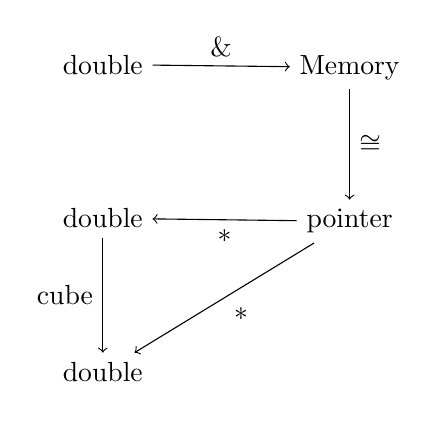
\begin{tikzpicture}
  \matrix (m) [matrix of math nodes, row sep=4em, column sep=5em, minimum width=2em]
  {
    \text{double} & \text{Memory} \\
    \text{double} & \text{pointer} \\
    \text{double} & \\ 
  };
  \path[->]
  (m-1-1) edge node [auto] {$\&$} (m-1-2)
  (m-1-2) edge node [right] {$\cong$} (m-2-2)
  (m-2-2) edge node [auto] {$*$} (m-2-1)
  edge node [auto] {$*$} (m-3-1)
  (m-2-1) edge node [left] {$\text{cube}$} (m-3-1)
  ;
 \end{tikzpicture} \qquad \qquad \,
  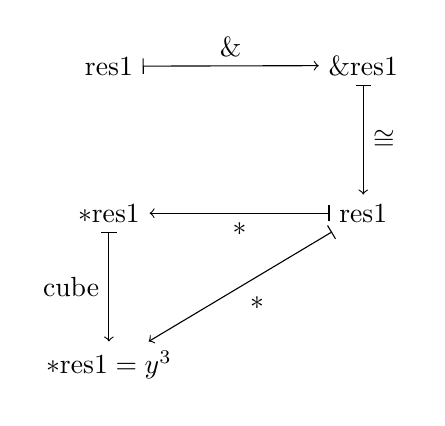
\begin{tikzpicture}
  \matrix (m) [matrix of math nodes, row sep=4em, column sep=5em, minimum width=2em]
  {
    \text{res1} & \&\text{res1} \\
    *\text{res1} & \text{res1} \\
    *\text{res1} = y^3 & \\ 
  };
  \path[|->]
  (m-1-1) edge node [auto] {$\&$} (m-1-2)
  (m-1-2) edge node [right] {$\cong$} (m-2-2)
  (m-2-2) edge node [auto] {$*$} (m-2-1)
  edge node [auto] {$*$} (m-3-1)
  (m-2-1) edge node [left] {$\text{cube}$} (m-3-1)
  ;
  \end{tikzpicture}
\]

It's unclear to me how \verb|void cube| can be represented in terms of category theory, as surely it cannot be represented as a mapping (it acts upon a functor, namely the $*$ functor for pointers).  It doesn't return a value, and so one cannot be confident to say there's explicitly a domain and codomain, or range for that matter.

But what is going on is that
\[
\begin{gathered}
  \text{ pointer }, \text{ double } , \text{ pointer } \xrightarrow{ \text{ cube } } \text{ pointer }, \text{ pointer } \\ 
  \text{fun}1, x , \text{res}1 \overset{\text{cube}}{\mapsto} \text{fun}1, \text{res}1
\end{gathered}
\]
s.t. $*\text{res}1 = y^3=(*\text{fun}1(x))^3$


So I'll speculate that in this case, \verb|cube| is a functor, and in particular, is acting on $*$, the so-called deferencing operator:
\[
\begin{gathered}
  \text{ pointer } \xrightarrow{ * } \text{float} \in \text{Data} \\
  \text{ res}1 \overset{*}{\mapsto} *\text{res}1
\end{gathered} \xrightarrow{ \text{ cube } } \begin{gathered}
  \text{ pointer } \xrightarrow{ \text{cube}(*) } \text{float} \in \text{Data} \\
  \text{ res}1 \overset{\text{cube}(*)}{\mapsto} \text{cube}(*\text{res}1)=y^3
\end{gathered}
\]

cf.  Arrays, from Fitzpatrick \cite{Fitz}

\[
\text{Types} \xrightarrow{ \text{ declaration } } \text{arrays}
\]
If $x\in \text{Obj}\text{arrays}$,
\[
\& x[0] \in \text{Memory} \xrightarrow{ == } x \in \text{ pointer } (\text{to 1st element of array})
\]


cf. Section 2.13 Character Strings from Fitzpatrick \cite{Fitz}

\begin{lstlisting}
  char word[20] = ``four''
  char *word = ``four''
\end{lstlisting}

cf. C$++$ extensions for C according to Fitzpatrick \cite{Fitz}
\begin{itemize}
\item simplified syntax to pass by reference pointers into functions
\item inline functions
\item variable size arrays \begin{lstlisting}
  int n;
  double x[n];
  \end{lstlisting}
\item complex number class
\end{itemize}


\subsubsection{Need a CUDA, C, C$++$, IDE?  Try Eclipse!}

This website has a clear, lucid, and pedagogical tutorial for using Eclipse: \href{https://www.fayewilliams.com/2011/06/28/creating-your-first-c-program-in-eclipse/}{	
Creating Your First C++ Program in Eclipse}.  But it looks like I had to pay.  Other than the well-written tips on the webpage, I looked up stackexchange for my Eclipse questions (I had difficulty with the Eclipse documentation).  

\part{Machine Learning with Deep Learning}

cf. Machine Learning - Introduction, from Coursera.  Dr. Andrew Ng.

\begin{enumerate}
\item Week 1
  \begin{itemize}
  \item Linear Regression with One Variable
    \begin{itemize}
    \item Model and Cost Function
      \begin{itemize}
      \item Model Representation
      \item Cost Function
      \item Cost Function - Intuition I
      \item Cost Function - Intuition II
      \end{itemize}
    \item Parameter Learning
      \begin{itemize}
      \item Gradient Descent
      \item Gradient Descent Intuition
        \item Gradient Descent For Linear Regression
        \end{itemize}
      \end{itemize}
    \end{itemize}
  \end{enumerate}

\section{Linear Regression}

cf. Linear Regression with One Variable

cf. \href{https://www.coursera.org/learn/machine-learning/lecture/db3jS/model-representation}{Model Representation; Week 1 Linear Regression with 1 Variable, Coursera Machine Learning, Ng}

For hypothesis $h$,
\[
\begin{aligned}
  & h_{\theta} : \mathbb{R}^d \to \mathbb{R} \\ 
  & h_{\theta} : x \mapsto   h_{\theta}(x)  \qquad \, \text{ (prediction of $y$ for $x$)}
  \end{aligned}
\]
$h_{\theta} \in L(\mathbb{R}^d, \mathbb{R})$

\[
\begin{aligned}
  & h_{\theta} : \mathbb{R}^{ | \theta | } \to L(\mathbb{R}^d , \mathbb{R})  \\ 
  &  \theta \mapsto h_{\theta}
  \end{aligned}
\]

\href{https://www.coursera.org/learn/machine-learning/lecture/rkTp3/cost-function}{Cost Function; Week 1, Coursera, Machine Learning, Ng}

So for parameters
\[
\theta \in \mathbb{R}^{ |\theta| }
\]
define a \emph{cost function}
\begin{equation}
  J(\theta) = \frac{1}{2 m} \sum_{i=1}^m (h_{\theta}(x_i) - y_i)^2 
\end{equation}

In \href{http://cs229.stanford.edu/notes/cs229-notes1.pdf}{CS229 Lecture notes, Andrew Ng, for Supervised learning, Part I Linear Regression}, this least-squares cost function gives rise to the \textbf{ordinary least squares} regression model.  

Find
\[
\min_{\theta} J(\theta) = ? (???)
\]
for
\[
J : \mathbb{R}^{ |\theta| } \to \mathbb{R}
\]

Actually,
\begin{equation}
  \begin{aligned}
    & J(\theta, (x_i, y_i)_{i \in I_{\text{train}}} ) \\ 
    & J: \mathbb{R}^{ |\theta|} \times (\mathbb{R}^d)^m \times \mathbb{R}^m \to \mathbb{R}
    \end{aligned}
 \end{equation}
$m=$ number of training examples $= |I_{\text{train}}|$.  

Considering
\[
H(\theta + \Delta \theta ) \approx J(\theta) + \text{grad}J(\theta) \cdot \Delta \theta + \frac{1}{2t} \| \Delta \theta \|^2
\]
Suppose $\Delta \theta \equiv \Delta \theta(t) = t\Delta \theta$

$\Delta \theta \approx - \gamma \text{grad}J(\theta)$ is an ansatz, $\gamma$ small enough.

Then assume $J$ convex, use this ansatz by plugging in, with Lipshitz condition
\[
\| \text{grad}J(\theta + \Delta \theta) - \text{grad}J(\theta) \| \leq L \| \Delta \theta \| 
\]
some constant $L > 0$,

\begin{equation}
\begin{aligned}
  & \theta_{n+1}^i = \theta^i_n - \gamma_n (\text{grad}J(\theta))^i \\ 
 & \gamma_n = \frac{ (\theta^i_n - \theta^i_{n-1} ) (\text{grad}_{\theta}J(x_n) - \text{grad}_{\theta}J(x_{n-1}))^i }{ \| \text{grad}_{\theta} J(x_n) - \text{grad}_{\theta}J(x_{n-1})\|^2 } = \frac{ (\theta_n - \theta_{n-1} )\cdot  (\text{grad}_{\theta}J(x_n) - \text{grad}_{\theta}J(x_{n-1})) }{ \| \text{grad}_{\theta} J(x_n) - \text{grad}_{\theta}J(x_{n-1})\|^2 }
  \end{aligned}
  \end{equation}

or as Ng points out in the \href{https://www.coursera.org/learn/machine-learning/supplement/2GnUg/gradient-descent}{Gradient Descent lesson recap}, the correct way is to store in temporary variables first:

\begin{equation}
\begin{aligned}
  & \text{temp}  = \theta^i_n - \gamma_n (\text{grad}J(\theta))^i \\
  & \theta^i_{n+1} = \text{temp}
\end{aligned}
\end{equation}
where $\text{temp} \in \mathbb{R}^{|\theta|}$

In the lesson recap for \href{https://www.coursera.org/learn/machine-learning/supplement/QKEdR/gradient-descent-intuition}{Gradient Descent Intuition}, Ng denotes the learning rate $\alpha \in \mathbb{R}$ with $\alpha$, but note that it's denoted as $\gamma$ or \verb|gamma| for \verb|sci-kit learn|.  So be aware of different notations.  Nevertheless, the learning rate can be a constant, but even then, choosing it is nontrivial.

\subsubsection{Testing many hypotheses at the same time, via refactoring the matrix}

In \href{https://www.coursera.org/learn/machine-learning/lecture/dpF1j/matrix-matrix-multiplication}{Linear Algebra Review of Week 1, Matrix Matrix Multiplication}, Ng provided a useful tip in refactoring the matrix of hypotheses $h_{\theta}$ so to test multiple number of hypotheses at the same time on the same input data, $X$.

Mathematically, beginning with

\[
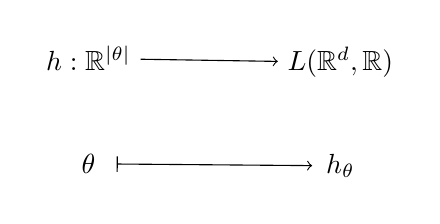
\begin{tikzpicture}
  \matrix (m) [matrix of math nodes, row sep=2.1em, column sep=5em, minimum width=2em]
  {
  h: \mathbb{R}^{ |\theta| } & L(\mathbb{R}^d, \mathbb{R}) \\
    \theta  & h_{\theta}  \\ 
  };
  \path[->]
  (m-1-1) edge node [auto] {$$} (m-1-2)
  ;
  \path[|->]
  (m-2-1) edge node [auto] {$$} (m-2-2)
  ;
  \end{tikzpicture}
\]
Consider testing $H$ different hypotheses, $\underbrace{\mathbb{R}^{ |\theta|} \times \dots \times \mathbb{R}^{ |\theta|} }_{H} \equiv \otimes_{i=1}^H \mathbb{R}^{ |\theta | }$,

so treat
\[
\otimes_{i=1}^H \mathbb{R}^{|\theta| } = \text{Mat}_{\mathbb{R}}(|\theta|,H)
\]
and so
\[
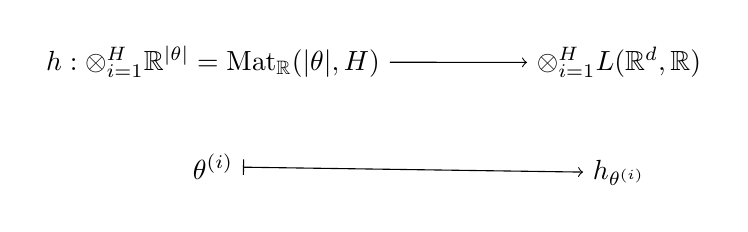
\begin{tikzpicture}
  \matrix (m) [matrix of math nodes, row sep=2.1em, column sep=5em, minimum width=2em]
  {
  h: \otimes_{i=1}^H \mathbb{R}^{ |\theta| } = \text{Mat}_{\mathbb{R}}(|\theta|,H)  & \otimes_{i=1}^H L(\mathbb{R}^d, \mathbb{R}) \\
    \theta^{(i)}  & h_{\theta^{(i)}}  \\ 
  };
  \path[->]
  (m-1-1) edge node [auto] {$$} (m-1-2)
  ;
  \path[|->]
  (m-2-1) edge node [auto] {$$} (m-2-2)
  ;
\end{tikzpicture}
\]


cf. \href{https://www.coursera.org/learn/machine-learning/lecture/OAOhO/non-linear-hypotheses}{Week 4, Non-linear Hypotheses video of Motivations for Coursera's Machine Learning by Ng}

For a sigmoid function $g$, consider
\[
g(\theta_0 + \theta_1 x_1 + \theta_2 x_2 + \theta_3 x_1 x_2 + \theta_4 x_1^2 x_2 + \theta_5 x_1^3 x_2 + \theta_6 x_1 x_2^2 + \dots ) 
\]
If $n$ large (Ng's notation), $d=\text{dim}\mathbb{R}^d$, number of features for training (data) set, \\
for including quadratic features,
\[
\begin{gathered}
\begin{aligned}
  & x_1^2, x_1x_2, x_1 x_3 , x_1 x_4 \dots x_1 x_{100} \\ 
  & x_2^2 , x_1x_3, \dots 
  \end{aligned} \\
\approx \mathcal{O}(n^2) \approx \frac{n^2}{2}  \qquad \, (\mathcal{O}(d^2) \approx \frac{d^2}{2} )
\end{gathered}
\]

e.g. computer vision, \\
e.g. $50 \times 50 $ pixel images, \\
$n=2500$ \\
 pixel intensity $\in [0,255] $ \\ 
 rgb $ \in [0,255]^3$

 \[
\begin{aligned}
  g:\mathbb{R}^{ |\theta| } & \to L(\mathbb{R}^d,\mathbb{R}) \\ 
 \theta & \mapsto g(\theta) \equiv g_{\theta}
\end{aligned}
\]
$n \equiv d=2$.

Consider
\[
\sum_{ \substack{ a_1,a_2 =0 \\ i=a_1 + 2a_2 } } \theta^{(i)}x_1^{a_1} x_2^{a_2} 
\]
and so for this example
\[
g(\theta)(x_1,x_2) = g\left( \sum_{ \substack{ a_1,a_2=0 \\ i=a_1+2a_2 } } \theta^{(i)}x_1^{a_1} x_2^{a_2} \right)
\]

For computer vision, consider
\[
x\in \mathbb{R}^d \text{ with } d = n^x \times n^y 
\]
and in particular, given pixel intensity or rgb range,
\[
\begin{aligned}
  & x\in [0,255]^d \\ 
  & x\in [0,255]^{3d}
\end{aligned}
\]

 



cf. \href{https://www.coursera.org/learn/machine-learning/supplement/Bln5m/model-representation-i}{Model Representation I of Week 4, Coursera's Machine Learning Introduction with Ng}

The notes at the end of each video segment \textbf{help very much}.

For input
\[
\mathbf{x} \in \mathbb{R}^d
\]
e.g. $d=1,2,3,\text{ or } 4, \dots $

$x_0  = $ ``bias unit'', input node 0, $x_0 =1$ always (Ng).


Sigmoid (logistic) activation function $\equiv a$.

\[
a_i^{(j)} \equiv \text{ ``activation'' of unit $i$ in layer $j$ }
\]
$j \in \lbrace 2, \dots , N-1 \rbrace$, $j=1$ is input layer, $j=N$ is output layer.

\[
a_i^{(j)} = g(\Theta_{ik}^{(j-1)} x_k)
\]

\[
j\xrightarrow{ \Theta^{(j)} } j+1 
\]
$\Theta^{(j)}$ matrix of weights controlling function mapping from layer $j$ to layer $j+1$.
\[
h_{\Theta}(x) = a_1^{(N)} = g(\Theta_{1k}^{(N-1)} a_k^{(N-1)} )
\]
$\forall \, $ layer $j$, $\exists \, $ matrix of weights $\Theta^{(j)}$.

If $s_j$ units in layer $j$, $s_{j+1}$ units in layer $j+1$, $\text{dim}\Theta^{(j)} = s_{j+1} \times (s_j + 1)$


If $N=2$, (1 neuron or only 1 hidden layer)

\[
\begin{gathered}
  x = (x_i)_{i=1 \dots d} \in \mathbb{R}^d, \qquad \, y \in \mathbb{R} , \, x_0 =1 \\ 
 y = h(\Theta_{1k}^{(1)} x_k^{(1)} ) = h(\Theta_{1k}^{(1)}x_k) = h(\Theta^{(1)} )(x)
  \end{gathered}
\]
e.g. $h(z) = \frac{1}{ 1 + e^z} $ logistic function.

Neural Network, input layer, output layer, and hidden layers.

\begin{equation}
  \Theta_{ik}^{(j)}x_k \mapsto g a_i^{(j+1)}   \qquad \, \begin{aligned} & k = 0,1, \dots s_j \\
    & i = 1,2, \dots s_{j+1} \end{aligned}
  \end{equation}

Note that $y$ can be $y \in \mathbb{R}^M$, not just $M=1$.


\href{https://www.coursera.org/learn/machine-learning/supplement/YlEVx/model-representation-ii}{Model Representation II}

$z_i^{(j)}$, $i=1, \dots s_j$, layer $j=1, \dots N$.

\begin{equation}
  g: z_i^{(j)} \mapsto a_i^{(j)}
  \end{equation}

e.g. $z_i^{(j)} = \Theta_{ik}^{(j-1)} x_k$, $k=0,1\dots d$.

Set $x=a^{(1)}$ for input layer.

\begin{equation}
  \begin{gathered}
    \Theta^{(j-1)} \in \text{Mat}_{\mathbb{R}}( (d+1), s_j) \\
    \Theta^{(j-1)} : a^{(j-1)} \in \mathbb{R}^{d+1} \mapsto z^{(j)} \in \mathbb{R}^{s_j} \xrightarrow{ g} a^{(j)} \in \mathbb{R}^{s_j} \xrightarrow{ a_0^{(j)} = 1 } a^{(j)} \in \mathbb{R}^{s_j + 1}
    \end{gathered}
  \end{equation}

For the $j=N$ case, ``output'' layer,
\begin{equation}
\begin{gathered}
  \Theta^{(N-1)} : a^{(N-1)} \mapsto z^N \in \mathbb{R} \xrightarrow{ g} g(z^N) = a^N = h_{\Theta}(x) \in \mathbb{R} \qquad \, \Theta^{(N-1)} \in \text{Mat}_{\mathbb{R}}( s_{N-1} +1, 1)
  \end{gathered}
  \end{equation}
In general,
\[
\begin{gathered}
  \Theta^{(N-1)} : a^{(N-1)} \mapsto z^N \in \mathbb{R} \xrightarrow{ g} g(z^N) = a^N = h_{\Theta}(x) \in \mathbb{R}^M \qquad \, \Theta^{(N-1)} \in \text{Mat}_{\mathbb{R}}( s_{N-1} +1, M)
\end{gathered}
\]



cf. \href{https://www.coursera.org/learn/machine-learning/lecture/CipHf/learning-with-large-datasets}{Learning With Large Datasets}, Quiz of Week 10, Gradient Descent with Large Datasets; Learning with Large Datasets.

Suppose you are facing a supervised learning problem and have a very large dataset ($m=100,000,000$).  How can you tell if using all of the data is likely to perform much better than using a small subset of the data (say $m=1,000$)?

Plot a learning curve ($J_{\text{train}}(\theta)$ and $J_{CV}(\theta)$, plotted as a function of $m$) for a range of values of $m$ and verify that the algorithm has high variance when $m$ is small.  


%for some range of values of $m$ (say up to $m=1,000$) and verify that the algorithm has bias when $m$ is small.


cf. 1.4 Regularized cost function

\[
\begin{gathered}
  J(\theta) = \frac{1}{m} \sum_{i=1}^m \sum_{k=1}^K \left[ -y_k^{(i)} \log{ ((h_{\theta}(x^{(i)} ) )_k ) } - (1-y_k^{(i)} ) \log{ (1- (h_{\theta}(x^{(i)} ) )_k ) } \right] + \\
+ \frac{\lambda}{2m} \left[ \sum_{j=1}^{s_2} \sum_{ k=1}^{ d} (\Theta_{j,k}^{(1)} )^2 + \sum_{j=1}^{K} \sum_{k=1}^{s_2} (\Theta^{(2)}_{j,k} )^2 \right]
  \end{gathered}
\]

\section{Logistic Regression; "logits"}  

Consider the problem of dealing with \emph{categorical} data.  I don't like the use of this name because it shouldn't be confused with category theory, or categories in category theory.  Nor should classes or types be used since they mean specific things in software design/object-oriented programming.  

Nevertheless, reasonably, we should assume a finite number of "categories" or "classes", $K$.  They have no \emph{ordering} properties, despite the fact that we will soon label the classes with numbers $0,1,\dots K-1$ or $1,2,\dots K$ (complicating things is how Python and C/C++ uses so-called $0$-based counting, i.e. counting from $0$, as opposed to how we're used to $1$-based counting).  So "categorical" or "classes" labels or names belong to the category of all finite sets, $\textbf{FiniteSets}$.  

The point I want to make is that in nearly all practical applications, we have to go from $\textbf{FiniteSets}$ to $\textbf{Vec}$: 
\begin{equation}
\begin{gathered}
\textbf{FiniteSets} \to \textbf{Vec}   \\
	\lbrace a_{i_1} \dots a_{i_K} \rbrace_{i_1\dots i_K \in \mathcal{I} } \to \lbrace 0,1,\dots K-1 \rbrace \to \delta_{ij}
\end{gathered}
\end{equation}

\subsection{Negative log likelihood function, for logistic regression}

cf. \href{http://deeplearning.net/tutorial/logreg.html}{Classifying MNIST digits using Logistic Regression}  

Look at the code \href{http://deeplearning.net/tutorial/code/logistic_sgd.py}{logistic sgd.py}.  Look at the function \verb|negative_log_likelihood|.  The math for that is this:

\begin{equation}
            \frac{1}{|\mathcal{D}|} \mathcal{L} (\theta=\{W,b\}, \mathcal{D}) =
            \frac{1}{|\mathcal{D}|} \sum_{i=0}^{|\mathcal{D}|}
                \log(P(Y=y^{(i)}|x^{(i)}, W,b)) \\
            \ell (\theta=\{W,b\}, \mathcal{D})
\end{equation}

Consider the cost function $J$ for a deep neural network (i.e. artificial neural network) for the case of "categorical" or "discrete" data, 
\begin{equation}
\begin{gathered}
	J(\mathbf{\Theta}) = \frac{1}{m} \sum_{i=1}^m \sum_{k=1}^K \left[ -y_k^{(i)} \log{ ((h_{\theta}(x^{(i)} ) )_k ) } - (1-y_k^{(i)} ) \log{ (1- (h_{\theta}(x^{(i)} ) )_k ) } \right] + \\
+ \frac{\lambda}{2m} \left[  \sum_{l=1}^L \sum_{j_{l-1}=0}^{s_{l-1}-1} \sum_{ j_l=0}^{ s_l-1} \left[  ( \Theta^{j_{l-1}}_{ \  \  \  j_l} )^{(l)}   \right]^2 \right] \qquad \, \text{ where } \\
(\Theta^j_{ \  \  k} )^{(l)}  \in (\mathbb{K}^{ s_{l-1}} ) \otimes ( \mathbb{K}^{s_l} )^* \cong \text{Mat}_{\mathbb{K}}(s_{l-1},s_l)  \qquad \, \text { for } \\
\begin{aligned}
	& l=1,2,\dots L \\ 
& j = 0,1,\dots s_{l-1} - 1 \\ 
& k = 0,1,\dots s_l - 1 
\end{aligned}
\end{gathered}
\end{equation}
Now for some particular $i$, $i\in 0,1,\dots m-1$ (where $m$ is the total number of input samples, i.e. "training examples" or "batch"), 
\[
y^{(i)} \in \lbrace 0 ,1 \rbrace^K 
\]
which represents the label or "class", or so-called "category" that the data pt. belongs to.  

The values that $y^{(i)}$ takes is such that if for the $i$th data sample, with it belongs specifically in "class" that's labeled $k'=0,1,\dots K-1$, then 
\[
y^{(i)}_k = \delta_{kk'}
\]
In this case, this is the so-called "1-hot vector representation."  

For example, suppose $K=10$.  We have 10 different "classes" or "categories" that a data point can belong in.  For a concrete example, take a digit that could be from 0 or to 9.  For any finite set we have an isomorphism to a subset of the integers; choose $\lbrace 0 ,1,\dots K-1\rbrace$.  Then we can represent the output or "target" $y$ to either take values from $\lbrace 0 ,1,\dots K-1\rbrace$ or turn it equivalently into a vector of length $K$ of $0$s and $1$s: e.g. if the digit is 3, then we can represent $y^{(i)}$ as $[0,0,0,1,0,0,0,0,0,0]$.  In this way, we can use \emph{activation} functions such as $\tanh$, softmax, sigmoid functions, etc. to get our DNN to compute an estimate of the probability that an input example belongs to each of the "categories".    






\section{Activation functions}

From wikipedia article on "Activation Function":

\[
\begin{gathered}
\begin{aligned}
\text{sigmoid } & f(x) = \frac{1}{ 1+ \exp{(-x)} } \in (0,1) & \begin{aligned} f'(x) & = -(1+e^{-x})^{-2} (-e^{-x}) \\ & = \left( \frac{1}{f(x)} -1\right)(f(x))^2 \\ & = f(x)(1-f(x)) \end{aligned} \\
	& f\in C^{\infty}  &  \\
& f(x) = \tanh{(x)} = \frac{2}{1+ e^{-2x}} -1 \in (-1,1) & f'(x) = \text{sech}^2(x) = 1-(f(x))^2 \in (0,1] \\ 
& f\in C^{\infty} & \\
& f(x) = \arctan{(x)} \in \left( \frac{-\pi}{2}, \frac{\pi}{2} \right) & f'(x) = \frac{1}{x^2 + 1} \in \left(\frac{1}{ \left( \frac{\pi}{2} \right)^2 + 1}, 1 \right) \\ 
& f\in C^{\infty} & \\
\begin{aligned} & \text{ReLu}, \\ & \text{Rectified linear unit} \end{aligned} & f(x) = \begin{cases} 0 & \text{ for } x < 0 \\ x & \text{ for } x \geq 0 \end{cases} \in [0,\infty) & f'(x) = \begin{cases} 0 & \text{ for } x <0 \\ 1 & \text{ for } x \geq 0 \end{cases} \\ 
& f \in C^1 &  \\ 
\text{Gaussian} & \begin{aligned} & f(x) = e^{-x^2} \in (0,1] ) \text{ or } \\
& f(x) = \exp{ \left( - \frac{ (x-c)^2}{ 2\sigma^2} \right) } \in (0,1] \end{aligned} &  f'(x) = -2xe^{-x^2} \\
& f\in C^{\infty} &
\end{aligned}
\end{gathered}
\]



\section{Feedforward; Feedforward Propagation and Prediction}

Given ordered sequence of linear transformations $L$, $L\geq 2$,
\begin{equation}
\begin{gathered}
  \Theta^{(l)} \in \text{Mat}_{\mathbb{R}}( s_l + 1, s_{l+1} ) \text{ i.e. } s_{l+1} \times (s_l +1) \text{ matrix size }, \, \forall \, l = 1,2, \dots L - 1  \\
  \begin{aligned}
    & \Theta^{(l)} : \mathbb{R}^{s_l +1} \to \mathbb{R}^{s_{l+1} } \\ 
    & \Theta^{(l)} : a^{(l)} \mapsto z^{(l+1) } = \Theta^{(l)} a^{(l)} = \Theta_{ij}^{(l)} a_j^{(l)} = z_i^{(l+1)}
    \end{aligned}
\end{gathered}
\end{equation}
$a^{(l)} \equiv $ ``activation'' of layer $l$.  

$s_l \equiv $ ``layer size'' of layer $l$, number of units or nodes in layer $l$

\begin{equation}
\begin{aligned}
  & g: \mathbb{R}^{s_l } \to \mathbb{R}^{s_l} \\ 
  & g : z^{(l)} \mapsto g(z^{(l)} )
  \end{aligned}
  \end{equation}
e.g. $g$ sigmoid function.

Remember to add $a_0^{(l)} = 1$, \, $\forall \, l = 1, \dots L-1$, i.e. $\forall \, $ input layer and hidden layers.

For $l=1$, the so-called \emph{input layer}, is such that
\begin{equation}
 (a_0^{(1)} = 1, x) = a^{(1)}
\end{equation}

For $l = 1,2, \dots L-1$,
\begin{equation}
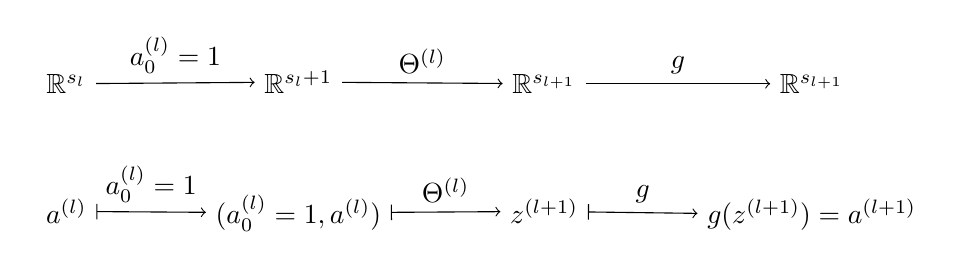
\begin{tikzpicture}
  \matrix (m) [matrix of math nodes, row sep=3em, column sep=4em, minimum width=2em]
  {
    \mathbb{R}^{s_l}  &  \mathbb{R}^{ s_l +1 }   & \mathbb{R}^{s_{l+1} } & \mathbb{R}^{s_{l+1} }  \\
a^{(l)} & (a_0^{(l)} = 1, a^{(l)} ) & z^{(l+1)} & g(z^{(l+1)}) = a^{(l+1)} \\
  };
  \path[->]
  (m-1-1) edge node [above] {$a_0^{(l)}=1$} (m-1-2)
  (m-1-2) edge node [above] {$\Theta^{(l)}$} (m-1-3)
  (m-1-3) edge node [above] {$g$} (m-1-4) 
  ;
  \path[|->]
  (m-2-1) edge node [above] {$a_0^{(l)}=1$} (m-2-2)
  (m-2-2) edge node [above] {$\Theta^{(l)}$} (m-2-3)
  (m-2-3) edge node [above] {$g$} (m-2-4) 
  ;
\end{tikzpicture}
  \end{equation}

\section{Backpropagation; Backpropagation algorithm}

\subsection{Backpropagation, gradient descent, for linear regression}  

Consider the particular form for linear regression:  
\[
\begin{gathered}
	\widehat{y}_{(i)}  \equiv h_{ (\Theta,b)}(X_{(i)}) \equiv h_{\Theta}(X_{(i)})=X_{(i)}\Theta + b \in \mathbb{R}^K \text{ or } \mathbb{R}^{s_1}, \qquad \, \forall \, i =1,2,\dots m (\text{index of input data $X$})
\end{gathered}
\]

Ng \cite{CS229} gives the gradient descent algorithm: 

\[
\Theta_{\mu}^{ \  \  \nu} \equiv \Theta_{\mu}^{ \  \  \nu}(t+1) := \Theta_{\mu}^{ \  \  \nu} - \alpha \frac{\partial }{ \partial \Theta_{\mu}^{ \  \  \nu} } J(\Theta,b)
\]
with $\alpha \equiv $ learning rate.  

And so given, with regularization term for full generality, $J(\Theta,b)$ of the form 
\[
\begin{aligned}
J(\Theta,b) & = \frac{1}{m} \sum_{i=1}^m J(\Theta,b; X_{(i)}, y_{(i)}) + \frac{\lambda}{2} \sum_{l=1}^L \sum_{i=0}^{s_{l-1}-1} \sum_{j=0}^{ s_l-1} ((\Theta^{(l)})^i_{\  \  j})^2 = \\ 
& =  \frac{ 1}{m} \sum_{i=1}^m \frac{1}{2} ( h_{(\Theta,b)}(X_{(i)}) - y_{(i)})^2 + \frac{\lambda}{2} \sum_{l=1}^L \sum_{i=0}^{s_{l-1}-1} \sum_{j=0}^{ s_l-1} ((\Theta^{(l)})^i_{\  \  j})^2
\end{aligned}
\]
with $h_{(\Theta,b)}(X_{(i)}) = x_{(i)}^{\mu} \Theta_{\mu}^{ \  \  \nu} + b^{\nu}$.  



As a programming note, anticipating that we have to do $\sum_{i=1}^m$ summation, employ a \emph{struct of arrays (SOA)}.  

\begin{equation}
\frac{\partial J(\Theta,b)}{ \partial \Theta_{\mu}^{ \  \  \nu} } = \frac{1}{m} \sum_{i=1}^m (\widehat{y}(X_{(i)}) - y_{(i)} )^{\nu} (X_{(i)})^{\mu} + \lambda \Theta_{\mu}^{ \  \  \nu} = \frac{1}{m} X(\widehat{y}(X) - y)^T + \lambda \Theta
\end{equation}
Notice how the matrix form $X(\widehat{y}(X) -y)^T$ works precisely because of the right-multiplication (order).  

The update is as follows, in component and matrix form:
\begin{equation}
\begin{gathered}
\Theta_{\mu}^{\  \  \nu}(t+1) := \Theta_{\mu}^{\  \  \nu}(t) - \alpha \frac{ \partial J( \Theta,b) }{ \partial \Theta_{\mu}^{\  \  \nu}}  = \Theta_{\mu}^{\  \  \nu}(t) - \alpha \frac{1}{m} \sum_{i=1}^m (\widehat{y}(X_{(i)}) - y_{(i)})^{\nu} (X_{(i)})^{\mu} + \lambda \Theta_{\mu}^{\  \  \nu} \\
\Theta(t+1) := \Theta(t) -\alpha \text{grad}_{\Theta}J = \Theta - \alpha \left( \frac{1}{m} X(\widehat{y}(X)-y)^T + \lambda \Theta \right) \\
b^{\nu}(t+1) := b^{\nu}(t) - \alpha \frac{ \partial J }{ \partial b^{\nu}} = b^{\nu}(t) - \alpha \frac{1}{m} \sum_{i=1}^m (\widehat{y}(X_{(i)}) - y_{(i)})^{\nu} 
\end{gathered}
\end{equation}

\subsection{Backpropagation, gradient descent, for artificial Neural Networks (NN)}
Recall the feedforward (i.e. composition of R-modules and Hadamard functions), and the resulting parameters (for the model).  These parameters belong to a space of parameters which in in itself is a differentiable manifold (so-called matrix manifold):  
\begin{equation}
\begin{gathered}
(\Theta,b) \in (\mathbf{\Theta},\mathbf{b}) \equiv \text{Mat}_{\mathbb{R}}(s_0,s_1) \times \mathbb{R}^{s_1} \times \text{Mat}_{\mathbb{R}}(s_1,s_2) \times \mathbb{R}^{s_2} \times \dots \times \text{Mat}_{\mathbb{R}}(s_{L-1},s_L) \times \mathbb{R}^{s_L} = \prod_{l=1}^L \text{Mat}(s_{l-1},s_l)\times \mathbb{R}^{s_l}  
\end{gathered}
\end{equation}
 
Also, recall what the cost functional does: 
\begin{equation}
\begin{aligned} 
& J:(\mathbf{\Theta}, \mathbf{b}) \to L((\mathbb{K}^d)^m,(\mathbb{K}^K)^m)   \\
& J:(\Theta,b) \mapsto J(\Theta,b) \equiv J_{(\Theta,b)} \equiv J_{\Theta}
\end{aligned}
\end{equation}
where \\
$d = $ number of features \\
$K=$ dim. of output \\
$m=$ number of training examples \\
$\mathbb{K} =$ field or set.  



First, do feedforward on \emph{each} training example $t$, i.e.
\begin{equation}
\begin{gathered}
  \forall \, t = 1,2 \dots m  \\
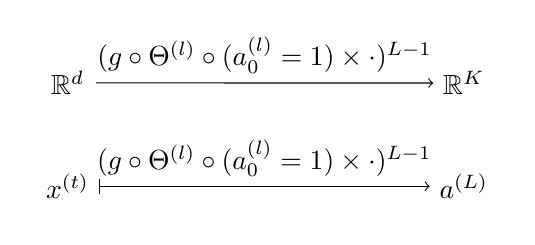
\begin{tikzpicture}
  \matrix (m) [matrix of math nodes, row sep=2.2em, column sep=12em, minimum width=2em]
  {
    \mathbb{R}^d & \mathbb{R}^K \\
    x^{(t)} & a^{(L)} \\
  };
  \path[->]
  (m-1-1) edge node [above] {$ (g \circ \Theta^{(l)} \circ (a_0^{(l)} = 1) \times \cdot )^{L-1}  $} (m-1-2)
  ;
  \path[|->]
  (m-2-1) edge node [above] {$ (g \circ \Theta^{(l)} \circ (a_0^{(l)} = 1) \times \cdot )^{L-1} $} (m-2-2)
  ;
\end{tikzpicture}
  \end{gathered}
  \end{equation}
For $K=1$ or $K>1$ e.g. $K=10$ for multi-class logistic regression.

In fact, we obtain an ordered sequence of ``activation'' vectors:

\begin{equation}
\begin{gathered}
  \forall \, t = 1,2 \dots m  \\
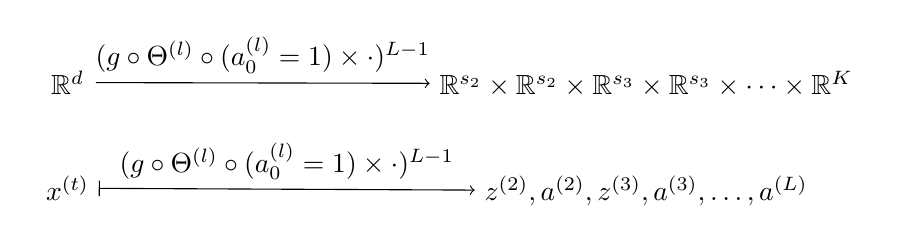
\begin{tikzpicture}
  \matrix (m) [matrix of math nodes, row sep=2.2em, column sep=12em, minimum width=2em]
  {
    \mathbb{R}^d & \mathbb{R}^{s_2} \times \mathbb{R}^{s_2} \times \mathbb{R}^{s_3} \times \mathbb{R}^{s_3} \times \dots \times \mathbb{R}^K \\
    x^{(t)} & z^{(2)}, a^{(2)}, z^{(3)}, a^{(3)}, \dots , a^{(L)} \\
  };
  \path[->]
  (m-1-1) edge node [above] {$ (g \circ \Theta^{(l)} \circ (a_0^{(l)} = 1) \times \cdot )^{L-1}  $} (m-1-2)
  ;
  \path[|->]
  (m-2-1) edge node [above] {$ (g \circ \Theta^{(l)} \circ (a_0^{(l)} = 1) \times \cdot )^{L-1} $} (m-2-2)
  ;
\end{tikzpicture}
  \end{gathered}
  \end{equation}

cf. \href{https://web.stanford.edu/class/cs294a/sparseAutoencoder_2011new.pdf}{CS294A Lecture notes, Andrew Ng, "Sparse autoencoder"}

Cleaning up the notation abit, and having the retrospective (wiser, more general) view, the setup is this:  

Given data to train on $(X,y) \in (\mathbb{K}^d \times \mathbb{K}^K)^m$, 
\begin{equation}
(X,y) \in (\mathbb{K}^d \times \mathbb{K}^K)^m \text{ where } \begin{aligned} & d = \text{ number of features } \\ 
	& K = \text{ dim. of output } \\
& m = \text{ number of training examples } \\ 
& \mathbb{K} = \text{ field or set }
\end{aligned}
\end{equation}

Consider weights and bias $(\Theta, b)$: 
\begin{equation}
	(\Theta, b) \in (\mathbf{\Theta}, \mathbf{b}) \equiv (\text{Mat}_{\mathbb{K}}(s_0,s_1) \times \mathbb{K}^{s_1} ) \times  (\text{Mat}_{\mathbb{K}}(s_1,s_2) \times \mathbb{K}^{s_2} ) \times \dots \times (\text{Mat}_{\mathbb{K}}(s_{L-1},s_L) \times \mathbb{K}^{s_L} )
\end{equation}
Consider the cost functional $\mathcal{J} := \mathcal{J}(\Theta,b)$ with the $L^1$ norm: 

\begin{equation}
\begin{aligned}
\mathcal{J}(\Theta,b) & = \left[ \frac{1}{m} \sum_{i=1}^m \mathcal{J}(\Theta,b; X_{(i)}, y_{(i)} ) \right] + \frac{\lambda}{2} \sum_{l=1}^L \sum_{i=0}^{s_{l-1} -1} \sum_{j=0}^{ s_l-1} ((\Theta^{(l)} )^i_{ \  \  j} )^2  \\
 &= \frac{1}{m} \sum_{i=1}^m \frac{1}{2} ( h_{(\Theta,b)}(X_{(i)} ) - y_{(i)} )^2 + \frac{\lambda}{2} \sum_{l=1}^L \sum_{i=0}^{s_{l-1}-1} \sum_{j=0}^{ s_l-1}  ((\Theta^{(l)})^i_{ \  \  j} )^2 
\end{aligned}
\end{equation}



1 iteration of gradient descent, $t=0,1,\dots $  

\begin{equation}
\begin{aligned}
&	(\Theta^{(l)})^i_{ \  \  j }(t+1)  = (\Theta^{(l)})^i_{ \  \  j}(t) - \alpha \frac{ \partial }{ \partial (\Theta^{(l)})^i_{ \  \  j} (t) } \mathcal{J}(\Theta,b) \qquad \, \begin{aligned}
	& \forall \, l =1,2,\dots L \\ 
	& \forall \, i = 0,1,\dots s_{l-1}- 1 \\ 
	&  \forall \, j = 0,1,\dots s_l - 1 
\end{aligned}
	& (b^{(l)})_j(t+1) = (b^{(l)})_j(t) - \alpha \frac{ \partial }{ \partial (b^{(l)} )_j (t) } J(\Theta,b)
\end{aligned}
\end{equation}

Consider the space of parameters $(\Theta,b) \in (\mathbf{\Theta}, \mathbf{b})$, 
\begin{equation}
(\Theta,b) \in (\mathbf{\Theta}, \mathbf{b}) \simeq \mathbb{R}^{ (s_0 + 1)s_1 + (s_1 +1)s_2 + \dots + (s_{L-1} + 1)s_L } \equiv \mathbb{R}^{ \sum_{l=1}^L (s_{l-1} + 1) s_l }
\end{equation}
Treat $(\mathbf{\Theta}, \mathbf{b})$ as a \emph{differentiable manifold}, as it is isomorphic to $\mathbb{R}^{ \sum_{l=1}^L (s_{l-1} + 1) s_l }$.  Note that while the data isn't necessarily in the format of a field, nor $\mathbb{R}$ for that matter, surely the parameter space $(\mathbf{\Theta},\mathbf{b})$ is.  

Assume that the cost functional is at least $C^1( (\mathbf{\Theta},\mathbf{b}) )$.  So 
\[
\begin{aligned}
&	\mathcal{J} : (\mathbf{\Theta},\mathbf{b}) \simeq \mathbb{R}^{ \sum_{l=1}^L (s_{l-1} + 1) s_l  } \to \mathbb{R}^1 \\ 
& 	\mathcal{J} : (\Theta,b) \mapsto \mathcal{J}( \Theta,b)
\end{aligned}
\]
Consider 1-jets of $\mathcal{J} : (\mathbf{\Theta},\mathbf{b}) \simeq \mathbb{R}^{ \sum_{l=1}^L  (s_{l-1} + 1)s_l } \to \mathbb{R}^1 \equiv J^1( (\mathbf{\Theta},\mathbf{b}) , \mathbb{R}) = (\mathbf{\Theta},\mathbf{b}) \times \mathbb{R}^1 \times \mathbb{R}^{ \sum_{l=1}^L (s_{l-1} + 1) s_l }$, i.e. treat $\mathcal{J}$ as section (or field)  $\mathcal{J} :  (\mathbf{\Theta},\mathbf{b}) \to (\mathbf{\Theta},\mathbf{b}) \times \mathbb{R}^1$.  

Then, we must compute $J^1_{\mathcal{J}}( (\Theta,b))$, the 1-jet, for some $(\Theta,b)$ (that is given in the beginning of the current iteration), the 1-jet of cost functional $\mathcal{J}$ at $(\Theta,b)$; it consists of $\sum_{l=1}^L (s_{l-1} + 1)s_l$ partial derivatives.  




From \href{https://www.coursera.org/learn/machine-learning/lecture/1z9WW/backpropagation-algorithm}{Backpropagation algorithm, Cost Function and Backpropagation, Week 5 of Coursera's Machine Learning Introduction by Ng}, \href{https://www.coursera.org/learn/machine-learning/supplement/pjdBA/backpropagation-algorithm}{Backpropagation algorithm} notes, and \verb|ex4.pdf|

Calculate
\begin{equation}
\begin{aligned}
  & \delta^{(L)} := a^{(L)} - y \\ 
  & \delta^{(L)}_k := a_k^{(L)} - y_k \qquad \, \forall \, k = 1,2, \dots K
  \end{aligned}
\end{equation}

For the term $((\Theta^{(L-1)})^T \delta^{(L)} )$, the matrix size dimensions of the $(\Theta^{(L-1)})^T$ are $\text{dim}( \Theta^{(L-1)} )^T = (s_{L-1}  + 1) \times s_L$.

It seems that the element-wise or component-wise multiplication that seems obvious in Matlab/Octave or numpy is called the \emph{Hadamard product}, denoted $\circ$ or $\odot$.  There ought to be a homomorphism that maps this operation onto ``vectorized'' forms of these vectors that allows for, or is equipped with the operation, Hadamard product.

For $m=1$,
\[
\delta^{(L-1)} := \left( ( \Theta^{(L-1)})^T \delta^{(L)} \right) \odot g'(z^{(L-1)}) \in \mathbb{R}^{s_{L-1} + 1} \qquad \, \forall \, k = 0 , 1, \dots s_{L-1}
\]
i.e.
\[
\begin{gathered}
  \text{vec}(\delta^{(L-1)} ) = \text{vec} ((\Theta^{(L-1)})^T \delta^{(L)} ) \odot \text{vec}( g'(z^{(L-1)}) ) \mapsto \delta^{(L-1)} \in \mathbb{R}^{s_{L-1} + 1} \\ 
 (s^{(L-1)} )_K := ((\Theta^{(L-1)})^T \delta^{(L)} )_K (g'(z^{(L-1)} ) )_K
\end{gathered}
\]

Then add this term to the so-called ``accumulator matrix'' $\Delta^{(l)}$:
\[
\Delta^{(l)} := \Delta^{(l)} + \delta^{(l+1)} (a^{(l)})^T
\]
Note that prior, skip or \emph{remove} $\delta_0^{(l+1)}$ entry:
\[
\delta^{(l+1)} \in \mathbb{R}^{ s_{l+1} + 1} \xrightarrow{ r} \delta^{(l+1)} \in \mathbb{R}^{s_{l+1} }
\]

The whole purpose is to obtain
\[
\frac{ \partial }{ \partial \Theta^{(l)}_{ij} } J(\Theta) = a_j^{(l)} \delta_i^{(l+1)} = a_j^{(l)} ( (\Theta^{(l+1)})^T \delta^{(l+2)} \odot g'(z^{(l+1)}) )_i  
\]
which can be shown.

So first we had set
\[
\Delta_{ij}^{(l)} = 0 
\]
for
\[
\Delta^{(l)} \in \text{Mat}_{\mathbb{R}}(s_l, s_{l+1} ) \in \mathbb{R}^{s_l} \otimes \mathbb{R}^{s_{l+1}} 
\]
Again, it can be shown that 
\begin{equation}
  \Delta_{ij}^{(l)} = \frac{ \partial }{ \partial \Theta^{(l)}_{ij} } J(\Theta)
  \end{equation}

and so
\[
\begin{aligned}
 & \Delta^{(l)} := \Delta^{(l)} + \delta^{(l+1)} (a^{(l)})^T \\ 
 & \Delta^{(l)}_{ij} := \Delta^{(l)}_{ij} + \delta^{(l+1)}_j (a^{(l)})_i 
\end{aligned}
\]
and so for $\forall \, t$,
\[
\begin{aligned}
\begin{cases}   D_{ij}^{(l)} := \frac{1}{m} \Delta_{ij}^{(l)} + \lambda \Theta_{ij}^{(l)} & \text{ if } j \neq 0 \\
  D_{ij}^{(l)} := \frac{1}{m} \Delta_{ij}^{(l)} & \text{ if } j = 0 \end{cases}
  \end{aligned}
\]
\[
D^{(l)} = \frac{1}{m} \sum_{t=1}^m (\Delta^{(l)})^{(t)} + \lambda \Theta^{(l)} \in \text{Mat}_{\mathbb{R}}(s_l,s_{l+1})
\]


In summary, we have, for the first step,
\begin{equation}
  \delta^{(L)} := a^{(L)} - y \in \mathbb{R}^K
  \end{equation}

\begin{equation}
  \delta^{(l)} = (\Theta^{(l)})^T \delta^{(l+1)} \odot g'(z^{(l)}) \in \mathbb{R}^{s_l + 1} , \qquad \, l = L-1,L-2, \dots 2, \qquad \, (L-2) \text{ steps } 
  \end{equation}

and so for
\begin{equation}
(\Delta^{(l)})^{(t)} := (\delta^{(l+1)}(a^{(l)})^T)^{(t)}
\end{equation}
\begin{equation}
D^{(l)} = \frac{1}{m} \sum_{t=1}^m (\Delta^{(l)})^{(t)}  + \lambda \Theta^{(l)} \in \text{Mat}^l_{\mathbb{R}}(s_l,s_{l+1})
\end{equation}
with $D^{(l)} \sim \frac{ \partial }{ \partial \Theta_{ij}^{(l)} } J(\Theta)$.

And so
\begin{equation}
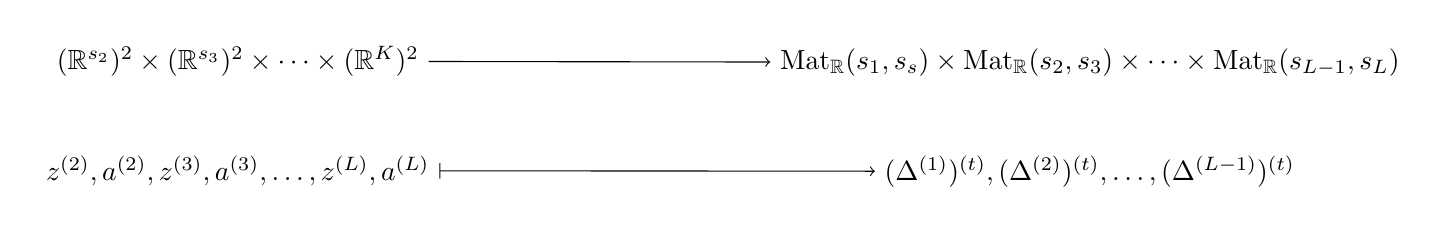
\begin{tikzpicture}
  \matrix (m) [matrix of math nodes, row sep=2.2em, column sep=12em, minimum width=2em]
         {
            (\mathbb{R}^{s_2})^2 \times (\mathbb{R}^{s_3})^2 \times \dots \times (\mathbb{R}^K)^2 & \text{Mat}_{\mathbb{R}}(s_1,s_s) \times \text{Mat}_{\mathbb{R}}(s_2,s_3) \times \dots \times \text{Mat}_{\mathbb{R}}(s_{L-1},s_L) \\
     z^{(2)}, a^{(2)}, z^{(3)}, a^{(3)}, \dots , z^{(L)}, a^{(L)} & (\Delta^{(1)})^{(t)}, (\Delta^{(2)})^{(t)}, \dots , (\Delta^{(L-1)})^{(t)} \\
  };
  \path[->]
  (m-1-1) edge node [above] {$    $} (m-1-2)
  ;
  \path[|->]
  (m-2-1) edge node [above] {$   $} (m-2-2)
  ;
\end{tikzpicture}
  \end{equation}
$\forall \, t = 1, \dots m$, then obtaining
\begin{equation}
  D^{(l)} \sim \frac{ \partial }{ \partial \Theta^{(l)}_{ij} }J(\Theta) \in \text{Mat}_{\mathbb{R}}(s_l,s_{l+1}) \qquad \, \forall \, l = 1,2, \dots L-1
  \end{equation}


To collect our facts, consider that we're given $x\in (\mathbb{R}^d)^m$, with $x_i^{(t)}$, $\begin{aligned} & \quad \\
  & i = 1 \dots d \\
  & t = 1 \dots m \end{aligned}$, with $\begin{aligned} & \quad \\
  & y\in (\mathbb{R}^K)^m \\
  & y \in \lbrace 1, 2, \dots K \rbrace^m \qquad \, (\text{classifier}) \end{aligned}$.

``layer'' $l=1,2, \dots L-1$
For input layer $\begin{aligned}
  & \Theta^{(1)} : \mathbb{R}^{d+1} \to \mathbb{R}^{s_2} \\
  & \Theta^{(1)}: a^{(1)} \mapsto \Theta^{(1)}a^{(1)} = z^{(1)} \end{aligned}$, with $a^{(1)} = (1,x^{(t)})$.

Instead of thinking of separate ``layers'', one should really think of encapsulating the relation, or arrows, or mappings between ``layers'':

\begin{equation}
 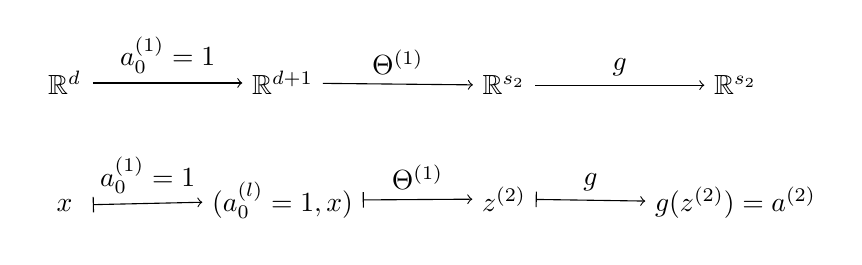
\begin{tikzpicture}
  \matrix (m) [matrix of math nodes, row sep=2.5em, column sep=4em, minimum width=2em]
  {
    \mathbb{R}^{d}  &  \mathbb{R}^{ d +1 }   & \mathbb{R}^{s_{2} } & \mathbb{R}^{s_{2} }  \\
x & (a_0^{(l)} = 1, x ) & z^{(2)} & g(z^{(2)}) = a^{(2)} \\
  };
  \path[->]
  (m-1-1) edge node [above] {$a_0^{(1)}=1$} (m-1-2)
  (m-1-2) edge node [above] {$\Theta^{(1)}$} (m-1-3)
  (m-1-3) edge node [above] {$g$} (m-1-4) 
  ;
  \path[|->]
  (m-2-1) edge node [above] {$a_0^{(1)}=1$} (m-2-2)
  (m-2-2) edge node [above] {$\Theta^{(1)}$} (m-2-3)
  (m-2-3) edge node [above] {$g$} (m-2-4) 
  ;
\end{tikzpicture}
\end{equation}


\begin{equation}
 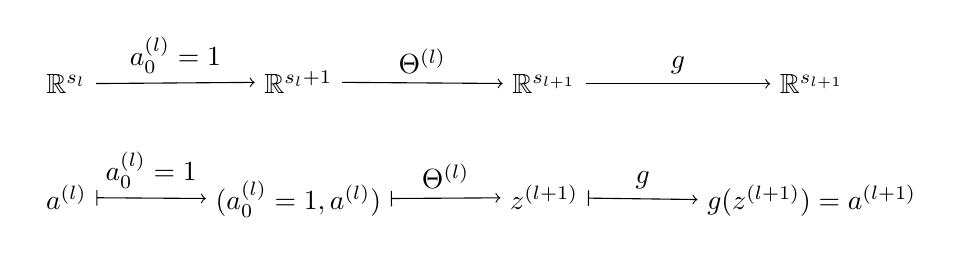
\begin{tikzpicture}
  \matrix (m) [matrix of math nodes, row sep=2.5em, column sep=4em, minimum width=2em]
  {
    \mathbb{R}^{s_l}  &  \mathbb{R}^{ s_l +1 }   & \mathbb{R}^{s_{l+1} } & \mathbb{R}^{s_{l+1} }  \\
a^{(l)} & (a_0^{(l)} = 1, a^{(l)} ) & z^{(l+1)} & g(z^{(l+1)}) = a^{(l+1)} \\
  };
  \path[->]
  (m-1-1) edge node [above] {$a_0^{(l)}=1$} (m-1-2)
  (m-1-2) edge node [above] {$\Theta^{(l)}$} (m-1-3)
  (m-1-3) edge node [above] {$g$} (m-1-4) 
  ;
  \path[|->]
  (m-2-1) edge node [above] {$a_0^{(l)}=1$} (m-2-2)
  (m-2-2) edge node [above] {$\Theta^{(l)}$} (m-2-3)
  (m-2-3) edge node [above] {$g$} (m-2-4) 
  ;
\end{tikzpicture}
\end{equation}

I found that Theano wasn't like the `\verb|.stack|` method, the ``addition'' of adding the $a_0=1$ component to a vector or matrix, as a shared variable, very much on the GPU (it indeed is a bug, \href{https://github.com/fchollet/keras/issues/152}{ Merge fails on GPU but passes on CPU \#152 }, and so I rewrote the mathematical formulation to fit in with separating the intercepts from the ``weights'' or $\Theta$.

For
\begin{equation}
\Theta^{(l)}, b^{(l)} : \mathbb{R}^{s_l} \to \mathbb{R}^{s_l+1}
\end{equation}
where
\begin{equation}
  \begin{aligned}
    & \Theta^{(l)} \in \text{Mat}_{\mathbb{R}}(s_l,s_{l+1}) = \mathbb{R}^{s_{l+1}} \otimes ( \mathbb{R}^{s_l})^* \\
    & b^{(l)} \in \mathbb{R}^{s_{l+1}}
    \end{aligned}
  \end{equation}
\begin{equation}
 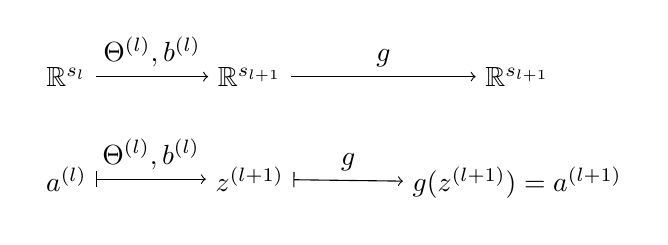
\begin{tikzpicture}
  \matrix (m) [matrix of math nodes, row sep=2.25em, column sep=4em, minimum width=2em]
  {
    \mathbb{R}^{s_l}  &   \mathbb{R}^{s_{l+1} } & \mathbb{R}^{s_{l+1} }  \\
a^{(l)} &   z^{(l+1)} & g(z^{(l+1)}) = a^{(l+1)} \\
  };
  \path[->]
  (m-1-1) edge node [above] {$\Theta^{(l)}, b^{(l)}$} (m-1-2)
  (m-1-2) edge node [above] {$g$} (m-1-3) 
  ;
  \path[|->]
  (m-2-1) edge node [above] {$\Theta^{(l)}, b^{(l)}$} (m-2-2)
  (m-2-2) edge node [above] {$g$} (m-2-3) 
  ;
\end{tikzpicture}
  \end{equation}

See also \href{https://web.stanford.edu/class/cs294a/}{CS294A/CS294W Deep Learning and Unsupervised Feature Learning Winter 2011}

\subsection{Backpropagation, gradient of the $L^2$ cost functional (linear regression)for gradient descent, for a DNN, in detail (chain rule on compositions)}

Given dataset $X,y$:
\[
\begin{aligned}
& X = X_i^{\  \  \mu} \in \text{Mat}_{\mathbb{R}}(m,d) \quad & i = 0,1, \dots m-1, \, \mu = 0,1,\dots d-1 \\ 
& y = y_i^{\  \  k} \in \text{Mat}_{\mathbb{R}}(m,K) \quad & i=0,1,\dots m-1, \, k=0,1,\dots K-1
\end{aligned}
\]

Start with 2 Axons (i.e. 1 "hidden" layer), $L=2$. Then $l=1,2$ (in general, $l=1,2,\dots L$).  

For $l=1$, 
\[
\begin{aligned}
& (z^{(1)})_i^{\  \  j_1} := X_i^{\  \  \mu} (\Theta^{(1)})_{\mu}^{\  \  j_1} + (b^{(1)})^{j_1}  & \in \text{Mat}_{\mathbb{R}}(m,s_1) \\
& (a^{(1)})_i^{\  \  j_1} := \psi^{(1)}( X_i^{\  \  \mu} (\Theta^{(1)})_{\mu}^{\  \  j_1} + (b^{(1)})^{j_1} ) & \in \text{Mat}_{\mathbb{R}}(m,s_1)
\end{aligned}
\]  
Likewise, for $l=2$, 
\[
\begin{aligned}
& (z^{(2)})_i^{\  \  j_2} := (a^{(1)})_i^{\  \  j_1} (\Theta^{(2)})_{j_1}^{\  \  j_2} + (b^{(2)})^{j_2}  & \in \text{Mat}_{\mathbb{R}}(m,s_2) \\
& (a^{(2)})_i^{\  \  j_2} := \psi^{(2)}( (a^{(1)})_i^{\  \  j_1} (\Theta^{(2)})_{j_1}^{\  \  j_2} + (b^{(2)})^{j_2} ) & \in \text{Mat}_{\mathbb{R}}(m,s_2)
\end{aligned}
\]  

Immediately, we can generalize:
\begin{equation}
\begin{aligned}
& (z^{(l)})_i^{\  \  j_l} := (a^{(l-1)})_i^{\  \  j_{l-1}} (\Theta^{(l)})_{j_{l-1}}^{\  \  j_l} + (b^{(l)})^{j_l}  & \in \text{Mat}_{\mathbb{R}}(m,s_l) \\
& (a^{(l)})_i^{\  \  j_l} := \psi^{(l)}( (a^{(l-1)})_i^{\  \  j_{l-1}} (\Theta^{(l)})_{j_{l-1}}^{\  \  j_l} + (b^{(l)})^{j_l} ) & \in \text{Mat}_{\mathbb{R}}(m,s_l)
\end{aligned}
\end{equation}

In general, for the $L^2$-norm cost functional $J$, the form is the following: 
\begin{equation}
\begin{aligned}
J(\Theta,b)  =  \frac{ 1}{m} \sum_{i=1}^m \frac{1}{2} ( a^{(L)}_i - y_{(i)})^2 + \frac{\lambda}{2} \sum_{l=1}^L \sum_{i=0}^{s_{l-1}-1} \sum_{j=0}^{ s_l-1} ((\Theta^{(l)})^i_{\  \  j})^2
\end{aligned}
\end{equation}
and this is also true:
\begin{equation}
\frac{ \partial }{ \partial (\Theta^{(l)})_j^{\  \  k} } \frac{1}{2} (a_i^{(L)} - y_{(i)})^2 = (a_i^{(L)} - y_{(i)}) \frac{\partial a_i^{(L)} }{ \partial (\Theta^{(l)})_j^{\  \  k} }
\end{equation}

For the sake of implementation, write out the $L^2$-norm cost functional $J$ explicitly:  
\[
\begin{gathered}
	\Delta \equiv \Delta_i^{\  \  k} \equiv (a_i^{(L)} - y_{(i)}) \equiv (a_i^{(L)} - y_{(i)})^k \in \text{Mat}_{\mathbb{R}}(m,K) \\ 
	 (a_i^{(L)} - y_{(i)})^2 \equiv (\Delta_i)^2 = \sum_{k=0}^{K-1}( \Delta_i^{\  \  k})^2 = \sum_{k=0}^{K-1} ((a_i^{(L)} - y_{(i)})^k)^2   \\
\sum_{i=1}^m (\Delta_i)^2 = \sum_{i=1}^m \sum_{k=0}^{K-1} (\Delta_i^{\  \  k})^2 = \sum_{i=1}^m \sum_{k=0}^{K-1} ((a_i^{(L)} - y_{(i)})^k)^2
\end{gathered}
\]

To get some intuition, let's do some simple examples.  Let $l=L$ and $L=2$:
\[
\frac{\partial a_i^{(L)} }{ \partial (\Theta^{(L)})_j^{\  \  k} } = \frac{ \partial \psi^{(L)} }{ \partial z^{(L)} }(z^{(L)} )  \frac{ \partial z^{(L)} }{ \partial (\Theta^{(L)})_j^{\  \  k} }= \frac{ \partial \psi^{(L)} }{ \partial ( z^{(L)})^k } (z^{(L)}  ) (a^{(L-1)})_i^{\  \  j} 
\]

Since $\psi^{(l)} \cdot$ is element-wise Hadamard operation, its dependence is only upon 1 element and we should exploit this fact.  

\[
\frac{\partial (a_i^{(L)})^k }{ \partial (\Theta^{(L)})_j^{\  \  m} } = \frac{ \partial (z^{(L)})_i^{\  \  k} }{ \partial (\Theta^{(L)})_j^{\  \  m} }  \frac{ \partial (\psi^{(L)})_i^{\  \  k } }{ \partial (z^{(L)})_i^{\  \  k} }(z^{(L)} )   = (a^{(L-1)})_i^{\  \  j} \delta^{mk}  \frac{ \partial (\psi^{(L)})_i^{\  \  k } }{ \partial (z^{(L)})_i^{\  \  k} }
\]
or 
\[
\frac{\partial (a_i^{(L)})^k }{ \partial (\Theta^{(L)})_j^{\  \  k} } =  (a^{(L-1)})_i^{\  \  j}   \frac{ \partial (\psi^{(L)})_i^{\  \  k } }{ \partial (z^{(L)})_i^{\  \  k} }
\]
For $l=L-1$, 
\[
\begin{gathered}
\frac{\partial (a_i^{(L)})^k }{ \partial (\Theta^{(L-1)})_j^{\  \  m} } = \frac{ \partial (z^{(L)})_i^{\  \  k} }{ \partial (\Theta^{(L-1)})_j^{\  \  m} }  \frac{ \partial (\psi^{(L)})_i^{\  \  k } }{ \partial (z^{(L)})_i^{\  \  k} }   =  \frac{\partial (a_i^{(L-1)})^{j_{L-1} }}{ \partial (\Theta^{(L-1)})_j^{\  \  m} } \frac{ \partial (z^{(L)})_i^{\  \  k} }{ \partial ( a_i^{(L-1)})^{    j_{L-1}} }     \frac{ \partial (\psi^{(L)})_i^{\  \  k } }{ \partial (z^{(L)})_i^{\  \  k} } = \\
= (a^{(L-2)})_i^{\  \  j} \delta^{m j_{L-1}}  \frac{ \partial (\psi^{(L-1)})_i^{\  \  j_{L-1} } }{ \partial (z^{(L-1)})_i^{\  \  j_{L-1}} }  (\Theta^{(L)})_{ j_{L-1}}^{\  \  k}    \frac{ \partial (\psi^{(L)})_i^{\  \  k } }{ \partial (z^{(L)})_i^{\  \  k} } = \\ 
= (a^{(L-2)})_i^{\  \  j}    \frac{ \partial (\psi^{(L-1)})_i^{\  \  m } }{ \partial (z^{(L-1)})_i^{\  \   m } }  (\Theta^{(L)})_{ m }^{\  \  k}    \frac{ \partial (\psi^{(L)})_i^{\  \  k } }{ \partial (z^{(L)})_i^{\  \  k} }
\end{gathered}
\]

Doing 1 more, for $l=L-2$, 
\[
\begin{gathered}
\frac{\partial (a_i^{(L)})^k }{ \partial (\Theta^{(L-2)})_j^{\  \  m} } =  \left[  \frac{\partial (a_i^{(L-1)})^{j_{L-1} }}{ \partial (\Theta^{(L-2)})_j^{\  \  m} } \right]  (\Theta^{(L)})_{ j_{L-1}}^{\  \  k}      \frac{ \partial (\psi^{(L)})_i^{\  \  k } }{ \partial (z^{(L)})_i^{\  \  k} } = \\
= \left[ (a^{(L-3)})_i^{\  \  j} \delta^{m j_{L-2}}  \frac{ \partial (\psi^{(L-2)})_i^{\  \  j_{L-2} } }{ \partial (z^{(L-2)})_i^{\  \  j_{L-2}} }  (\Theta^{(L-1)})_{ j_{L-2}}^{\  \  j_{L-1}}    \frac{ \partial (\psi^{(L-1)})_i^{\  \  j_{L-1} } }{ \partial (z^{(L-1)})_i^{\  \  j_{L-1}} } \right]  (\Theta^{(L)})_{ j_{L-1}}^{\  \  k}      \frac{ \partial (\psi^{(L)})_i^{\  \  k } }{ \partial (z^{(L)})_i^{\  \  k} } = \\
=  (a^{(L-3)})_i^{\  \  j}    \frac{ \partial (\psi^{(L-2)})_i^{\  \  m } }{ \partial (z^{(L-2)})_i^{\  \   m } }  (\Theta^{(L-1)})_{ m }^{\  \  j_{L-1}}    \frac{ \partial (\psi^{(L-1)})_i^{\  \  j_{L-1} } }{ \partial (z^{(L-1)})_i^{\  \  j_{L-1}} }   (\Theta^{(L)})_{ j_{L-1}}^{\  \  k}      \frac{ \partial (\psi^{(L)})_i^{\  \  k } }{ \partial (z^{(L)})_i^{\  \  k} }
\end{gathered}
\]

And so in general, for $l=1,2,\dots L$, 
\begin{equation}
\boxed{ \begin{gathered}
\frac{\partial (a_i^{(L)})^k }{ \partial (\Theta^{(L-(l-1))})_j^{\  \  m} } =   (a^{(L-l)})_i^{\  \  j}    \frac{ \partial (\psi^{(L-(l-1))})_i^{\  \  m } }{ \partial (z^{(L-(l-1))})_i^{\  \   m } }  (\Theta^{(L-(l-2))})_m^{\  \  j_{(L-(l-2))}}      \frac{ \partial (\psi^{(L-(l-2))})_i^{\  \  j_{(L-(l-2))} } }{ \partial (z^{(L-(l-2))})_i^{\  \  j_{(L-(l-2))}} } \cdot \\
\cdot \prod_{l' = l-3}^{l'=1} (\Theta^{(L-l')})_{ j_{L-(l'+1)}}^{\  \  j_{L-l'}}      \frac{ \partial (\psi^{(L-l')})_i^{\  \  j_{L-l'} } }{ \partial (z^{(L-l')})_i^{\  \  j_{L-l'}} } \cdot (\Theta^{(L)})_{ j_{L-1}}^{\  \  k}      \frac{ \partial (\psi^{(L)})_i^{\  \  k } }{ \partial (z^{(L)})_i^{\  \  k} }
\end{gathered} 
}
\end{equation}

Indeed, by induction, 
\[
\begin{gathered}
\frac{\partial (a_i^{(L)})^k }{ \partial (\Theta^{(L-l))})_j^{\  \  m} } =  \left[  \frac{\partial (a_i^{(L-1)})^{j_{L-1} }}{ \partial (\Theta^{(L-l)})_j^{\  \  m} } \right]  (\Theta^{(L)})_{ j_{L-1}}^{\  \  k}      \frac{ \partial (\psi^{(L)}_i)^{\  \  k } }{ \partial (z^{(L)}_i)^{\  \  k} } = \\
= (a^{(L-1-l)}_i)^{\  \  j}    \frac{ \partial (\psi_i^{(L-1-(l-1))})^{\  \  m } }{ \partial (z_i^{(L-(l-1))})^{\  \   m } }  (\Theta^{(L-(l-1))})_m^{\  \  j_{(L-(l-1))}}      \frac{ \partial (\psi_i^{(L-(l-1))})^{\  \  j_{(L-(l-1))} } }{ \partial (z_i^{(L-(l-1))})^{\  \  j_{(L-(l-1))}} } \cdot \\
\cdot \prod_{l' = l-3}^{l'=1} (\Theta^{(L-1-l')})_{ j_{L-1-(l'+1)}}^{\  \  j_{L-1-l'}}      \frac{ \partial (\psi^{(L-1-l')}_i)^{\  \  j_{L-1-l'} } }{ \partial (z^{(L-1-l')}_i)^{\  \  j_{L-1-l'}} } \cdot (\Theta^{(L-1)})_{ j_{L-2}}^{\  \  j_{L-1}}      \frac{ \partial (\psi_i^{(L-1)})^{\  \  j_{L-1} } }{ \partial (z_i^{(L-1)})^{\  \  j_{L-1}} } \cdot \\ 
\cdot (\Theta^{(L)})_{ j_{L-1}}^{\  \  k}      \frac{ \partial (\psi^{(L)}_i)^{\  \  k } }{ \partial (z^{(L)}_i)^{\  \  k} } = \\
= (a^{(L-1-l)}_i)^{\  \  j}    \frac{ \partial (\psi_i^{(L-1-(l-1))})^{\  \  m } }{ \partial (z_i^{(L-(l-1))})^{\  \   m } }  (\Theta^{(L-(l-1))})_m^{\  \  j_{(L-(l-1))}}      \frac{ \partial (\psi_i^{(L-(l-1))})^{\  \  j_{(L-(l-1))} } }{ \partial (z_i^{(L-(l-1))})^{\  \  j_{(L-(l-1))}} } \cdot \\
\cdot \prod_{l' = l-2}^{l'=1} (\Theta^{(L-l')})_{ j_{L-(l'+1)}}^{\  \  j_{L-l'}}      \frac{ \partial (\psi^{(L-l')}_i)^{\  \  j_{L-l'} } }{ \partial (z^{(L-l')}_i)^{\  \  j_{L-l'}} } \cdot (\Theta^{(L)})_{ j_{L-1}}^{\  \  k}      \frac{ \partial (\psi^{(L)}_i)^{\  \  k } }{ \partial (z^{(L)}_i)^{\  \  k} } 
\end{gathered}
\]


As a check, consider the $L=1$ case with no activation function, \emph{linear regression}, 
\[
\frac{ \partial (a_i^{(1)})^k }{ \partial \Theta_j^{\  \  m}} = (a^{(0)}_i)^j \delta^{mk} 1
\]
And so,
\[
\begin{gathered}
\frac{\partial J}{ \partial ( \Theta^{(l)})_j^{\  \  p} } = \frac{1}{m} \sum_{i=1}^m (a_i^{(L)} - y_{(i)} ) \frac{\partial a_i^{(L)} }{ \partial ( \Theta^{(l)})_j^{\  \  p} } + \lambda ( \Theta^{(l)})_j^{\  \  p} \equiv \frac{1}{m} \sum_{i=1}^m \Delta _i \frac{\partial a_i^{(L)} }{ \partial  ( \Theta^{(l)})_j^{\  \  p} } + \lambda ( \Theta^{(l)})_j^{\  \  p} =\\
= \frac{1}{m} \sum_{i=1}^m \sum_{k=0}^{K-1} \Delta_i^{\  \  k} \frac{ \partial ( a_i^{(L)})^k }{ \partial ( \Theta^{(l)})_j^{\  \  p}} + \lambda ( \Theta^{(l)})_j^{\  \  p} 
\end{gathered}
\]

For the linear regression case, we have
\[
\Delta_i^{\  \  k} (a_i^{(0)})^j \delta^{pk} = \Delta_i^{\  \  p} (a_i^{(0)})^j 
\]
or explicitly 
\[
\sum_{k=0}^{K-1} \Delta_i^{\  \  k} (a_i^{(0)})^j \delta^{pk} = \Delta_i^{\  \  p} (a_i^{(0)})^j
\]
and so, for this linear regression case,  
\begin{equation}
\frac{ \partial J}{ \partial ( \Theta)_j^{\  \  p}} = \frac{1}{m} \sum_{i=1}^m \Delta_i^{\  \  p} (a_i^{(0)})^j + \lambda \Theta_j^{\  \  p}
\end{equation}

\subsubsection{Backpropagation of bias $b$, for $L^2$ norm cost functional $J$}

\[
\begin{gathered}
\begin{aligned}
& \frac{ \partial }{ \partial (b^{(l)})^p} \frac{1}{2} (a_i^{(L)} - y_{(i)})^2 = (a_i^{(L)} - y_{(i)} ) \frac{ \partial a_i^{(L)} }{ \partial (b^{(l)})^p } \\
& \frac{ \partial ( a_i^{(L)})^k }{ \partial (b^{(L)})^p}  = \delta_p^{\  \  k} \frac{ \partial ( \psi^{(L)})_i^{\  \  k} }{ \partial (z^{(L)})_i^{\  \  k} } = \frac{ \partial ( \psi^{(L)})_i^{\  \  p} }{ \partial (z^{(L)})_i^{\  \  p})}  \\
 & \frac{ \partial ( a_i^{(L)})^k }{ \partial (b^{(L-1)})^p} = \frac{ \partial (z^{(L)})_i^{\  \  k} }{ \partial ( b^{(L-1)})^p} \frac{\partial (\psi^{(L)}_i)^k }{ \partial (z^{(L)})_i^{\  \  k} } = \frac{ \partial (a_i^{(L-1)})^{j_{L-1}} }{ \partial (b^{(L-1)})^p }  \frac{ \partial (z^{(L)})_i^{\  \  k} }{ \partial ( a^{(L-1)})^{j_{L-1}}  }\frac{\partial (\psi^{(L)}_i)^k }{ \partial (z^{(L)})_i^{\  \  k} }  =  \delta^{p j_{L-1}} \frac{ \partial ( \psi_i^{(L-1)})^{j_{L-1}} }{ \partial (z^{(L-1)})_i^{\  \  j_{L-1} } }  ( \Theta^{(L)})_{j_{L-1}}^{\  \  k}   \frac{\partial (\psi^{(L)}_i)^k }{ \partial (z^{(L)})_i^{\  \  k} } = \\
 & = \frac{ \partial ( \psi_i^{(L-1)})^{ p } }{ \partial (z^{(L-1)})_i^{\  \  p } }  ( \Theta^{(L)})_{ p }^{\  \  k}   \frac{\partial (\psi^{(L)}_i)^k }{ \partial (z^{(L)})_i^{\  \  k} }   \\
& \frac{ \partial ( a_i^{(L)})^k }{ \partial (b^{(L-2)})^p} = \frac{ \partial (a_i^{(L-1)})^{j_{L-1}} }{ \partial (b^{(L-2)})^p }  (\Theta^{(L)})_{j_{L-1}}^{\  \  k}  \frac{\partial (\psi^{(L)}_i)^k }{ \partial (z^{(L)})_i^{\  \  k} }  = \\
& = \frac{ \partial ( \psi_i^{(L-2)})^{ p } }{ \partial (z^{(L-2)})_i^{\  \  p } }  ( \Theta^{(L-1)})_{ p }^{\  \  j_{L-1}}    \frac{\partial (\psi^{(L-1)}_i)^{j_{L-1}} }{ \partial (z^{(L-1)})_i^{\  \  j_{L-1}} }   (\Theta^{(L)})_{j_{L-1}}^{\  \  k}  \frac{\partial (\psi^{(L)}_i)^k }{ \partial (z^{(L)})_i^{\  \  k} }
\end{aligned}
\end{gathered}
\]
Suppose 
\begin{equation}
\boxed{ \begin{gathered}
\frac{ \partial ( a_i^{(L)})^k }{ \partial (b^{(L-(l-1))})^p} = \frac{ \partial ( \psi_i^{(L-(l-1))})^{ p } }{ \partial (z^{(L-(l-1))})_i^{\  \  p } }  ( \Theta^{(L-(l-2))})_{ p }^{\  \  j_{L- (l-2)  }} \prod_{l'=l-2}^{l'=2 }  \frac{ \partial ( \psi_i^{(L-l'+1)})^{ j_{L-l'} } }{ \partial (z^{(L-l'+1)})_i^{\  \  j_{L-l'} } }  ( \Theta^{(L-l'+1)})_{ j_{L-l'} }^{\  \  j_{L-l'+1}} \cdot \\
\cdot \frac{ \partial ( \psi_i^{(L-1)})^{ j_{L-1} } }{ \partial (z^{(L-1)})_i^{\  \  j_{L-1} } }  ( \Theta^{(L)})_{ j_{L-1} }^{\  \  k} \frac{ \partial ( \psi_i^{(L)})^{ k } }{ \partial (z^{(L)})_i^{\  \  k } }       
\end{gathered} }
\end{equation}

Indeed, by induction, 
\[
\begin{gathered}
\frac{ \partial ( a_i^{(L)})^k }{ \partial (b^{(L-l)})^p} = \frac{ \partial ( a_i^{(L-1)})^{ j_{L-1} } }{ \partial (b^{(L-l)})^{    p } }  ( \Theta^{(L)})_{ j_{L-1} }^{\  \  k} \frac{ \partial ( \psi_i^{(L)})^{ k } }{ \partial (z^{(L)})_i^{\  \  k } }   = \\
=  \frac{ \partial ( \psi_i^{(L-l))})^{ p } }{ \partial (z^{(L-l))})_i^{\  \  p } }  ( \Theta^{(L-(l-1))})_{ p }^{\  \  j_{L- (l-1)  }} \prod_{l'=l-2}^{l'=2 }  \frac{ \partial ( \psi_i^{(L-l')})^{ j_{L-1-l'} } }{ \partial (z^{(L-l')})_i^{\  \  j_{L-1-l'} } }  ( \Theta^{(L-l')})_{ j_{L-1-l'} }^{\  \  j_{L-l'}} \cdot \\
\cdot \frac{ \partial ( \psi_i^{(L-1)})^{ j_{L-2} } }{ \partial (z^{(L-1)})_i^{\  \  j_{L-2} } }  ( \Theta^{(L-1)})_{ j_{L-2} }^{\  \  L-1} \frac{ \partial ( \psi_i^{(L-1)})^{ j_{L-1} } }{ \partial (z^{(L-1)})_i^{\  \  j_{L-1} } } ( \Theta^{(L)})_{ j_{L-1} }^{\  \  k} \frac{ \partial ( \psi_i^{(L)})^{ k } }{ \partial (z^{(L)})_i^{\  \  k } }       = \\
= \frac{ \partial ( \psi_i^{(L-l))})^{ p } }{ \partial (z^{(L-l))})_i^{\  \  p } }  ( \Theta^{(L-(l-1))})_{ p }^{\  \  j_{L- (l-1)  }} \prod_{l'=l-1}^{l'=2 }  \frac{ \partial ( \psi_i^{(L-l'+1)})^{ j_{L-l'} } }{ \partial (z^{(L-l'+1)})_i^{\  \  j_{L-l'} } }  ( \Theta^{(L-l'+1)})_{ j_{L-l'} }^{\  \  j_{L-l'+1}} \cdot  \frac{ \partial ( \psi_i^{(L-1)})^{ j_{L-1} } }{ \partial (z^{(L-1)})_i^{\  \  j_{L-1} } }  ( \Theta^{(L)})_{ j_{L-1} }^{\  \  k} \frac{ \partial ( \psi_i^{(L)})^{ k } }{ \partial (z^{(L)})_i^{\  \  k } }       
\end{gathered}
\]

For the linear regression case, 
\[
\frac{ \partial J}{ \partial b^p} = \frac{1}{m} \sum_{i=1}^m \Delta_i^{\  \  k } \delta_{pk} = \frac{1}{m} \sum_{i=1}^m \Delta_i^{\  \  p}
\]

\subsection{Backpropagation for the Negative log likelihood function, for logistic regression}

Recall the full expression for the cost functional of a deep neural network (DNN or ANN) using the negative log likelihood function (or so-called cross-entropy function):  

\begin{equation}
J(\Theta,b) = \frac{1}{m} \sum_{i=1}^m \sum_{k=1}^K \left[ -y^k_{(i)} \log{ (h^k_{(\Theta,b)}(x_{(i)}) )} - (1-y^k_{(i)}) \log{ (1-h^k_{(\Theta,b)}(x_{(i)}) )}  \right] +  \frac{\lambda}{2m} \left[ \sum_{l=1}^L \sum_{j_{l-1} =0}^{ s_{l-1} -1} \sum_{j_l =0}^{s_l - 1} \left[ ( \Theta^{ (l)} )_{j_l}^{j_{l-1}} \right]^2 \right]
\end{equation}

Define the so-called cross-entropy function $s$:
\[
\begin{aligned}
& s:[0,1]^2 \to \mathbb{R} \\ 
& s\equiv s( y^k_{(i)}, \widehat{y}_{(i)}^k ) = -y^k_{(i)} \log{ (\widehat{y}^k_{(i)})} - (1-y^k_{(i)}) \log{ (1-\widehat{y}^k_{(i)})}  
\end{aligned}
\]
$s$ notation was chosen to relate it, as it's formally equivalent, to entropy, whether the physical definition of entropy or Shannon entropy.  There ought to be a (succinct) mathematical discussion of how $s$ relates to Shannon entropy and to information theory.  Otherwise, from the physical point of view, the form of $s$ was chosen because of its mathematical properties ($s$ should be additive when we add 2 systems, $A$,$B$ together, etc.)

Taking the partial derivative and keeping in mind that $\widehat{y}_{(i)}^k = \widehat{y}_{(i)}^k(\Theta,b)$, (i.e. only $\widehat{y}_{(i)}^k$ is dependent upon $(\Theta,b)\in (\mathbf{\Theta},\mathbf{b})$, and nothing else, not $y^k_{(i)}$, the given output data, 
\[
\begin{gathered}
\frac{\partial s}{ \partial (\Theta^{ (L-(l-1))})_j^{\  \  p} } = -y^k_{(i)} \frac{1}{ \widehat{y}_{(i)}^k  } \frac{\partial \widehat{y}_{(i)}^k }{ \partial ( \Theta^{(L-(l-1))})_j^{\  \  p } } +  \frac{ (1- y^k_{ (i)}) }{ 1- \widehat{y}_{(i)}^k } \frac{\partial \widehat{y}_{(i)}^k }{ \partial (\Theta^{(L-(l-1))})_j^{\  \  p} } = \\
= \frac{ - y^k_{(i)} (1- \widehat{y}^k_{(i)}) + \widehat{y}^k_{(i)} (1-y^k_{(i)}) }{ \widehat{y}^k_{(i)} ( 1 - \widehat{y}^k_{(i)}) } \frac{\partial \widehat{y}_{(i)}^k }{ \partial (\Theta^{(L-(l-1))})_j^{\  \  p} } = \frac{\widehat{y}_{(i)}^k - y_{(i)}^k }{ \widehat{y}_{(i)}^k (1 - \widehat{y}_{(i)}^k )} \frac{\partial \widehat{y}_{(i)}^k }{ \partial (\Theta^{(L-(l-1))})_j^{\  \  p} }
\end{gathered}
\] 
In summary, 
\begin{equation}
\frac{\partial s}{ \partial (\Theta^{ (L-(l-1))})_j^{\  \  p} } = \frac{\widehat{y}_{(i)}^k - y_{(i)}^k }{ \widehat{y}_{(i)}^k (1 - \widehat{y}_{(i)}^k )} \frac{\partial \widehat{y}_{(i)}^k }{ \partial (\Theta^{(L-(l-1))})_j^{\  \  p} }
\end{equation}


Clearly, 
\begin{equation}
\frac{\partial s}{ \partial (b^{ (L-(l-1))})^{\  \  p} } = \frac{\widehat{y}_{(i)}^k - y_{(i)}^k }{ \widehat{y}_{(i)}^k (1 - \widehat{y}_{(i)}^k )} \frac{\partial \widehat{y}_{(i)}^k }{ \partial ( b^{(L-(l-1))})^{\  \  p} }
\end{equation}

\section{Cost functional}

The cost function $J$ is really a cost \emph{functional}, to first input in the output values $y$.  So
\begin{equation}
\begin{aligned}
  &  J: (\mathbb{R}^K)^m \to L(\mathbf{ (\Theta, b) }, \mathbb{R} ) \\ 
& J: y \mapsto J_y \equiv J 
\end{aligned}
\end{equation}
for a ``vector-valued'' regression, with the usual linear regression being the case of $K=1$.

For $y$ taking on discrete values,
\begin{equation}
\begin{aligned}
  & J: \lbrace 1, 2, \dots K \rbrace^m \to L( \mathbf{ (\Theta ,b) } , \mathbb{R} ) \\ 
  & J: y \mapsto J_y \equiv J 
  \end{aligned}
  \end{equation}
Then, we can find the cost $J((\Theta, b))$, for a particular choice of the parameters, $(\Theta,b) \in \mathbf{ (\Theta,b)}$:
\begin{equation}
\begin{aligned}
 &  J_y \equiv J : \mathbf{ ( \Theta,b) } \to \mathbb{R} \\ 
 & J: (\Theta,b) \to J(\Theta,b)
  \end{aligned}
  \end{equation}
i.e. $J \in C^{\infty}((\Theta,b))$ (hopefully $J$ is smooth or at least $C^2$ differentiable, so that a Hessian can be obtained).


For the above $\mathbf{ (\Theta,b)}$ was notation or shorthand as follows:

\[
\mathbf{ (\Theta,b ) } \equiv (\text{Mat}_{\mathbb{R}}(s_1,s_2) \times \mathbb{R}^{s_2}) \times (\text{Mat}_{\mathbb{R}}(s_2,s_3) \times \mathbb{R}^{s_3} ) \times \dots \times (\text{Mat}_{\mathbb{R}}(s_{L-1},s_L) \times \mathbb{R}^{s_L} )
\]

\section{Evaluating a Learning Algorithm, Model Selection, Cross-validation}  

cf. \href{https://www.coursera.org/learn/machine-learning/lecture/OVM4M/deciding-what-to-try-next}{Deciding what to Try Next} for Week 6, Evaluating a Learning Algorithm.  

Suppose we have a regularized linear regression model for supervised learning.  

\begin{equation}
	J(\Theta) = \frac{1}{2} \sum_{i=1}^m (h_{\Theta}(X_{(i)}) - y_{(i)} )^2 + \frac{\lambda}{2m} \sum_{j=1}^s \sum_{\mu=1}^d (\Theta_{\mu}^{\  \  \  j })^2 =  \frac{1}{2} \sum_{i=1}^m (h_{\Theta}(X_{(i)} ) - y_{(i)} )^2 + \frac{\lambda}{2m} \sum_{\mu =1}^d (\Theta_{\mu}^{ \  \  \  j })^2 
\end{equation}

For Model diagnosis, to answer questions of too great of error in $J$, \emph{do cross-validation}.  

So, \\

Do cross-validation.  For instance, given $X \in \mathbf{X} \in \text{Mod}_{R}$, $X_i^{ \  \  \mu } \in \mathbb{K}$, $\mathbf{X}_i \in \mathbb{K}^d$, \, $\forall \, i =1,2\dots m$, $\forall \, \mu =1\dots d$.  Do some random permutation on $(1,2,\dots m)$, and then split into training, validation, and test sets.  

Suppose from $J(\Theta)(X_{\text{train}})$, obtain $\Theta$ s.t. $\min_{\Theta} J(\Theta)(X_{\text{train}})$.  

Then $J_{\text{test}}(\Theta) = J(\Theta)(X_{\text{test}}) = \frac{1}{2} \sum_{i=1}^{m_{\text{test}}} (h_{\Theta}(X_i) - y_{(i)} )^2 + \frac{\lambda}{2m_{\text{test}}} \sum_{\mu=1}^d (\Theta_{\mu})^2 $.  

For classification, classification error (aka 0/1 misclassification error), essentially taking a fraction, define
\begin{equation}
	\text{err}(h_{\Theta}(X_{(i)} ), y_{(i)} ) := \begin{cases} 1 & \text{ if } h_{\Theta}(X_{(i)} ) \geq 0.5 \text{ and } y=0 \text{ or } h_{\Theta}(X_{(i)}) < 0.5 \text{ and } y=1 \\ 
0 & \text{ otherwise } \end{cases}
\end{equation}

\[
J(\Theta)(X) = \frac{1}{m} \sum_{i=1}^m \text{err}(h_{\Theta}(X_{(i)}), y_{(i)} )
\]


cf. \href{https://www.coursera.org/learn/machine-learning/supplement/aFpD3/evaluating-a-hypothesis}{Evaluating a hypothesis}

cf. \href{https://www.coursera.org/learn/machine-learning/lecture/QGKbr/model-selection-and-train-validation-test-sets}{Model Selection and Train/Validation/Test Sets}

Given $J$, consider $J(X)(\Theta) = J_X(\Theta)$, when choosing between $\Theta$, vs. $\Theta'$, for $X=X_{\text{valid}}$.  $J_{X_{\text{valid}}}(\Theta)$ and vary $\Theta$, different choices or models of $\Theta$ (nonlinear, polynomial features, weighted by different $\Theta$, for example), while keeping $X_{\text{valid}}$ fixed, and observe changes in $J$.  

e.g. for $L^2$ loss, 
\[
\begin{aligned}
	& J_{\text{train}}(\Theta) \equiv  J(X_{\text{train}})(\Theta) = J_{X_{\text{train}}}(\Theta) = \frac{1}{2m_{\text{train}}} \sum_{i=1}^{m_{\text{train}} } (h_{\Theta}(X_{(i)}) -y_{(i)} )^2 \\ 
	& J_{\text{valid}}(\Theta) \equiv  J(X_{\text{valid}})(\Theta) = J_{X_{\text{valid}}}(\Theta) = \frac{1}{2m_{\text{valid}}} \sum_{i=1}^{m_{\text{valid}} } (h_{\Theta}(X_{(i)}) -y_{(i)} )^2 \\
	& J_{\text{test}}(\Theta) \equiv  J(\Theta)(X_{\text{test}}) = J_{\Theta}(X_{\text{test}}) = \frac{1}{2m_{\text{test}}} \sum_{i=1}^{m_{\text{test}} } (h_{\Theta}(X_{(i)}) -y_{(i)} )^2 
\end{aligned}
\]

\subsection{Diagnosing bias vs. variance}

cf \href{https://www.coursera.org/learn/machine-learning/lecture/yCAup/diagnosing-bias-vs-variance}{Diagnosing bias vs. variance}  If you're running a learning algorithm, and it doesn't do as well as expected, it's either, almost always,
\begin{enumerate}
\item bias - underfit
\item high variance - overfit
\end{enumerate}

\subsubsection{Diagnosing bias vs. variance}

Consider 
\[
\begin{aligned}
	& J_{\text{train}}(\Theta) \equiv  J(X_{\text{train}})(\Theta) = J_{X_{\text{train}}}(\Theta) = \frac{1}{2m_{\text{train}}} \sum_{i=1}^{m_{\text{train}} } (h_{\Theta}(X_{(i)}) -y_{(i)} )^2 \\ 
	& J_{\text{valid}}(\Theta) \equiv  J(X_{\text{valid}})(\Theta) = J_{X_{\text{valid}}}(\Theta) = \frac{1}{2m_{\text{valid}}} \sum_{i=1}^{m_{\text{valid}} } (h_{\Theta}(X_{(i)}) -y_{(i)} )^2 
\end{aligned}
\]
If both $J_{X_{\text{train}}}$, $J_{X_{\text{valid}}}$ large, \textbf{bias} problem, $\Theta$ form is not complex enough.  \\
If $J_{X_{\text{train}}}$ low, ($(h_{\Theta}(X_{\text{train}}) -y_{\text{train}})^2$ small), but $J_{X_{\text{valid}}}$ high, \textbf{high variance}, $\Theta$ too complex, overfits on $X_{\text{train}}$.  

\href{https://www.coursera.org/learn/machine-learning/lecture/4VDlf/regularization-and-bias-variance}{Regularization and Bias/Variance}  

\subsubsection{e.g. Linear regression with regularization, and how $\lambda$ affects underfitting (high bias) or overfitting (high variance)}

If $\lambda$ large, as $\min_{\Theta} J(\Theta)$, then $\Theta$ small, i.e. $\Theta \approx 0$, and so $h_{\Theta}(X_{(i)}) \approx 0$.  $J$ large.  \textbf{high bias (underfit)}.  \\
If $\lambda$ small, \textbf{high variance, overfit}.  $J$ (deceptively) small.  

\subsubsection{Choosing the regularization parameter $\lambda$; try an arbitrary range of values of $\lambda$, minimize $J$ with respect to $\lambda$}.  

Consider
\[
J_{X_{\text{valid}}}(\Theta) \equiv J_{cv}(\Theta) = J(X_{\text{valid}})(\Theta) = J(X_{\text{valid}})(\Theta)(\lambda)
\]
Then 
\[
\min_{\lambda \in [0,10] }J_{X_{\text{valid}},\Theta}(\lambda)
\]

cf. \href{https://www.coursera.org/learn/machine-learning/lecture/Kont7/learning-curves}{Learning Curves}

Consider $J=J(\Theta)(X) = J_{\Theta}(X)$ and consider $\lim_{m\to \infty} J_{\Theta}(X)$ with $X= X_i$, $\forall \, i =1,2,\dots m$.  

Note that $\lim_{m_{\text{train}}\to \infty} J_{\Theta}(X_{\text{train}}) \to $ large, since $J_{\Theta}(X_{\text{train}}) \sim \frac{1}{2m_{\text{train}}} \sum_{i=1}^{m_{\text{train}}} (h_{\Theta}(X_{(i)}) -y_{(i)})^2$.  \\
But $\lim_{m_{\text{valid}} \to \infty} J_{\Theta}(X_{\text{valid}}) \to 0$.  




\section{Universal approximation theorem}

\href{https://en.wikipedia.org/wiki/Universal_approximation_theorem}{Wikipedia: Universal Approximation Theorem}

From Hornik (1991) \cite{Horn1991}, pp. 252, Section 2. Results,
\begin{equation}
  \mathcal{N}_k^{(n)}(\psi)  = \lbrace h :\mathbb{R}^k \to \mathbb{R} | h(x) =\sum_{j=1}^n \beta_j \psi(a_j'x- \theta_j) \rbrace
\end{equation}
with
$\begin{aligned}
  & a = (\alpha_1 , \dots \alpha_k) \\ 
 & x = ( \xi_1, \dots, \xi_k) 
  \end{aligned}
$ with $a' \equiv a^T \equiv $ transpose of $a$.  

For arbitrary number of hidden layers,
\[
\mathcal{N}_k(\psi) = \bigcup_{n=1}^{\infty}\mathcal{N}_k^{(n)}(\psi)
\]
The 2 very important theorems from Hornik (1991) are the following:
\begin{theorem}
If $\psi$ unbounded and nonconstant, then $\mathcal{N}_k(\psi)$ dense in $L^p(\mu)$, $\forall \, $ finite measure $\mu$ on $\mathbb{R}^k$
\end{theorem}
\begin{theorem}
  If $\psi$ cont., bounded, nonconstant, then $\mathcal{N}_k(\psi)$ dense in $C(X)$, \, $\forall \,$ compact subsets $X$ of $\mathbb{R}^k$, \\
  i.e. $\forall \, f\in C(X)$, $\exists \, $ sequence, $(h_n)$ s.t. $h_n \xrightarrow{n} f$ uniformly i.e. $\forall \, $ given $\epsilon >0$, $\exists \, N=N(\epsilon)$ (independent of $x\in X\subset \mathbb{R}^k$), s.t. \\
  $|h_n(x)-f(x)| < \epsilon$ \, $\forall \, x \in X$, \, $\forall \, n \geq N(\epsilon)$
  \end{theorem}
I will write now a dictionary between Hornik's notation and my notation (take note, Hornik's notation $\equiv$ my notation).  

$f\in C(X)$, $f:\mathbb{R}^k\to \mathbb{R}$, $k\equiv d$, so $f:\mathbb{R}^d \to \mathbb{R}$ \\
 
$\psi \equiv g$, e.g. $g(z) = \frac{1}{1 + \exp{(-z)} }$ or $g(z) = \tanh{(z)}$, but equip $g$ with element-wise (component-wise) action, i.e. $g$ as a functor, $\begin{aligned} & \quad \\ 
    & g:\mathbb{R}^k \to \mathbb{R}^k \\
    & g:x_j\mapsto g(x_j) \end{aligned}$, i.e. $g: \mathbf{Vec} \to \mathbf{Vec}$.


  Now $a \equiv \Theta \in \text{Mat}_{\mathbb{R}}(d,n)$,
  \[
g(\Theta x + b) = g(z)
\]
i.e. $z\in \mathbb{R}^n$,
\[
z:= \Theta x + b \text{ i.e. } z_j = \Theta_{jk} x_k + b_j \qquad \, g(z) \in \mathbb{R}^n
\]
and so, notation-wise,
\[
\sum_{j=1}^n \beta_j \psi(a_j'x  - \theta_j) \equiv \sum_{j=1}^n \beta_j g(\Theta_{jk} x_k +b_j)
\]
Consider
\[
\begin{aligned}
  & \Theta^{(1)} \in \text{Mat}_{\mathbb{R}}(d,s_2), \, b^{(1)} \in \mathbb{R}^{s_2} \\ 
  & \Theta^{(2)} \in \text{Mat}_{\mathbb{R}}(s_2,1) , \, b^{(2)} \in \mathbb{R}
\end{aligned}
\]
\[
h(x) = \Theta^{(2)}g( \Theta^{(1)}x + b^{(1)}) + b^{(2)} \in \mathcal{N}_d^{(s_2)}(g)
\]
so the neural net of $L$ total layers $d=1$ ``input layer'', $l=L$ is ``output layer'' is a tuple $((\Theta,b),g)\in \mathcal{N}_d^{(L)}(g)$

Hornik, Stinchcombe, and White (1989) \cite{HSW1989} deals with multi-(hidden) layer networks on pp. 363, on and after Corollary 2.6.

Given training data,
\begin{equation}
  \begin{aligned}
    & (X,y) : \mathbb{R} \to (\mathbb{R}^d \times \mathbb{R}^k)^m \\ 
    & (X,y)(t) \mapsto (X(t),y(t))
    \end{aligned}
\end{equation}
discretize time $t\in \mathbb{R}$,
\begin{equation}
  \begin{aligned}
    \mathbb{R} &  \xrightarrow{ \text{ discretize }} \mathbb{Z} \\
 [0,T]\text{ where $T \in \mathbb{R}^+$ } & \to \lbrace 0 , 1, \dots T-1 \rbrace \text{ where } T\in \mathbb{Z}^+
    \end{aligned}
  \end{equation}

Consider 4 different feedforwards.  Note $y(-1)=0$.

\section{LSTM; Long Short Term Memory}

\href{http://www.christianherta.de/lehre/dataScience/machineLearning/neuralNetworks/LSTM.php}{LSTM (Long Short Term Memory), according to Christian Herta}

Rewriting Herta's formulation of LSTM, which actually puts in the ``cell'' memory into some of the input, forget gates, that's different from a ``traditional'' LSTM (see Wikipedia),
\begin{equation}
  \begin{aligned}
    \text{ input gates } & i_t = \psi_{(i)}(\Theta^{(i)}X_t + b^{(i)} + \theta^{(i)}h_{t-1} + W^{(i)}c_{t-1}) \\
        & f_t = \psi_{(f)}  (\Theta^{(f)} X_t + b^{(f)} + \theta^{(f)} h_{t-1} + W^{(f)} c_{t-1} )  \\
    & c_t := f_t \odot c_{t-1} + i_t \odot g_t \\
  \text{ output gates }   & o_t = \psi_{(0)} ( \Theta^{(0)} X_t + b^{(0)} + \Theta^{(0)} g_{t-1} + W^{(0)} c_t)
    \end{aligned}
  \end{equation}
and then finally, not predict yet (I was mistaken) but $h$ here denotes some other ``hidden'' variable,
\begin{equation}
  h_t = o_t\odot \psi_h(c_t)
\end{equation}


$o_t,c_t \in\mathbb{R}^H$, and so $W^{(i)}, W^{(f)}, W^{(0)} \in \text{Mat}_{\mathbb{R}}(H,s_2)$.

\begin{equation}
  \begin{aligned}
& y_t = \psi_{(y)}(\Theta^{(y)}h_t + b^{(y)} ) \\
& \Theta^{(y)}:\mathbb{R}^{s_L} \to \mathbb{R}^K
\end{aligned}
  \end{equation}

\begin{equation}
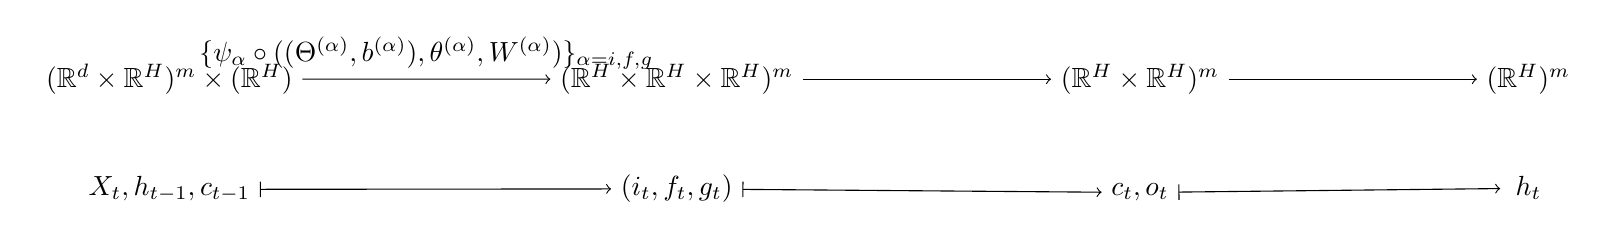
\begin{tikzpicture}
  \matrix (m) [matrix of math nodes, row sep=2.25em, column sep=9em, minimum width=2em]
  {
 (\mathbb{R}^d \times \mathbb{R}^H)^m \times (\mathbb{R}^H) & (\mathbb{R}^H \times \mathbb{R}^H \times \mathbb{R}^H)^m & (\mathbb{R}^H \times \mathbb{R}^H)^m & (\mathbb{R}^H)^m \\
X_t,h_{t-1},c_{t-1}  & (i_t,f_t,g_t) & c_t,o_t & h_t \\
  };
  \path[->]
  (m-1-1) edge node [above] {$\lbrace \psi_{\alpha}\circ ((\Theta^{(\alpha)},b^{(\alpha)}),\theta^{(\alpha)},W^{(\alpha)} ) \rbrace_{\alpha=i,f,g}$} (m-1-2)
  (m-1-2) edge node [above] {$$} (m-1-3)
    (m-1-3) edge node [above] {$$} (m-1-4) 
  ;
  \path[|->]
  (m-2-1) edge node [above] {$$} (m-2-2)
  (m-2-2) edge node [above] {$$} (m-2-3)
  (m-2-3) edge node [above] {$$} (m-2-4)
  ;
\end{tikzpicture}
  \end{equation}

Consider what we're essentially doing at time step $t$:
\begin{equation}
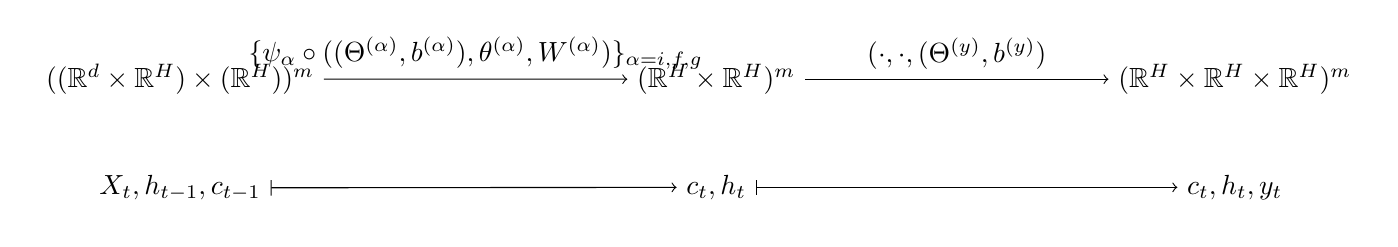
\begin{tikzpicture}
  \matrix (m) [matrix of math nodes, row sep=2.25em, column sep=11em, minimum width=2em]
  {
 ((\mathbb{R}^d \times \mathbb{R}^H) \times (\mathbb{R}^H))^m & (\mathbb{R}^H \times \mathbb{R}^H)^m & (\mathbb{R}^H \times \mathbb{R}^H \times \mathbb{R}^H )^m   \\
X_t,h_{t-1},c_{t-1}  & c_t,h_t & c_t, h_t,y_t \\
  };
  \path[->]
  (m-1-1) edge node [above] {$\lbrace \psi_{\alpha}\circ ((\Theta^{(\alpha)},b^{(\alpha)}),\theta^{(\alpha)},W^{(\alpha)} ) \rbrace_{\alpha=i,f,g}$} (m-1-2)
  (m-1-2) edge node [above] {$ (\cdot, \cdot, (\Theta^{(y)},b^{(y)})$} (m-1-3)
  ;
  \path[|->]
  (m-2-1) edge node [above] {$$} (m-2-2)
  (m-2-2) edge node [above] {$$} (m-2-3)
  ;
\end{tikzpicture}
  \end{equation}

The recurrence relation is essentially this:
\begin{equation}
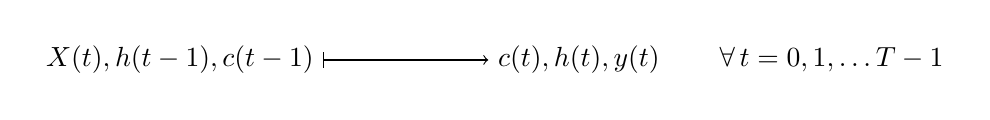
\begin{tikzpicture}
  \matrix (m) [matrix of math nodes, row sep=2.25em, column sep=6em, minimum width=2em]
  {
X(t),h(t-1),c(t-1) & c(t),h(t),y(t) \qquad \, \forall \, t = 0,1,\dots T-1 \\ 
  };
%  \path[->]
%  (m-1-1) edge node [above] {$\lbrace \psi_{\alpha}\circ ((\Theta^{(\alpha)},b^{(\alpha)}),\theta^{(\alpha)},W^{(\alpha)} ) \rbrace_{\alpha=i,f,g}$} (m-1-2)
%  ;
  \path[|->]
  (m-1-1) edge node [above] {$$} (m-1-2)
  ;
\end{tikzpicture}
  \end{equation}
This is the recurrence relation that changes with time $t$ and in the language of \verb|theano|, for \verb|theano.scan| it is the argument value for argument  \verb|sequences|.  

Notice how $h,c$ change over time.  These are the sequences we want to take in as input and output.  $X(t)$ is the sequences we want to ``iterate over.''  $X(t)$ doesn't get modified by our operations over time $t$ (than what is given).  $y(t)$ is an output we desire.  So in the language of \verb|theano|, for \verb|theano.scan|, $X(t)$ goes to the argument value for argument \verb|sequences|, as it's part of the ``list of Theano variables or dictionaries describing the sequences \verb|scan| has to iterate over'' and since $X=X(t)$ for time $t$, the ``\verb|taps|'' is \verb|[0]|.  $h,c,y$ is expected to be the return value of the Python function describing a single time step, and ``the order of the outputs is the same as the order of \verb|outputs_info|.  

Look at the parameters:
\begin{equation}
\begin{aligned}
  & (\Theta^{(g)},b^{(g)}), \theta^{(g)} \in (\text{Mat}_{\mathbb{R}}(d,H) \times \mathbb{R}^H \times \text{Mat}_{\mathbb{R}}(H,H) \\ 
  & (\Theta^{(\alpha)},b^{(\alpha)}), \theta^{(\alpha)}, W^{(\alpha)} \in (\text{Mat}_{\mathbb{R}}(d,H) \times \mathbb{R}^H \times \text{Mat}_{\mathbb{R}}(H,H) \times \text{Mat}_{\mathbb{R}}(H,H) \\
   & (\Theta^{(y)},b^{(y)})  \in (\text{Mat}_{\mathbb{R}}(H,K) 
  \end{aligned}
  \end{equation}
These parameters are what you put into, in the language of \verb|theano|, for the argument value of \verb|non_sequences| of \verb|theano.scan|.  

\subsection{Representation of time-dependent input and target data, i.e. when $X$ and $y$ depend on time $t$; Sequential data}

Consider this representation:  
\begin{equation}
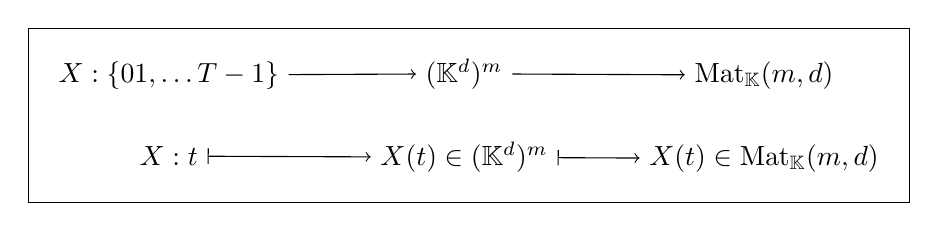
\begin{tikzpicture}[framed]
  \matrix (m) [matrix of math nodes, row sep=1.25em, column sep=3em, minimum width=1em]
  {
	X:\lbrace 0 1,\dots T-1 \rbrace & (\mathbb{K}^d)^m    & \text{Mat}_{\mathbb{K}}(m,d) \\
	X:t & X(t) \in (\mathbb{K}^d)^m & X(t) \in \text{Mat}_{\mathbb{K}}(m,d)  \\
  };
  \path[->]
  (m-1-1) edge node [above] {$$} (m-1-2)
	(m-1-2) edge node [above] {$$} (m-1-3)
  ;
  \path[|->]
  (m-2-1) edge node [above] {$$} (m-2-2)
(m-2-2) edge node [above] {$$} (m-2-3)
  ;
\end{tikzpicture}
\end{equation}
where $T,m,d\in\mathbb{Z}^+$.  

For clarification, note that $\forall \, t\in \lbrace 0 ,1,\dots T-1\rbrace$, i.e. every (discrete) time $t$, we have $m$ samples to consider: 
\[
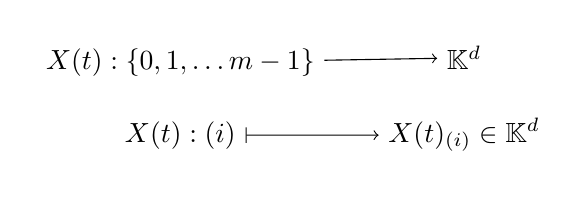
\begin{tikzpicture}
  \matrix (m) [matrix of math nodes, row sep=0.85em, column sep=2em, minimum width=.6em]
  {
	X(t) : \lbrace 0,1,\dots m -1\rbrace  & \mathbb{K}^d \\ 
	X(t): (i) & X(t)_{(i)} \in \mathbb{K}^d \\ 
  };
  \path[->]
  (m-1-1) edge node [above] {$$} (m-1-2)
  ;
  \path[|->]
  (m-2-1) edge node [above] {$$} (m-2-2)
  ;
\end{tikzpicture}
\]
\[
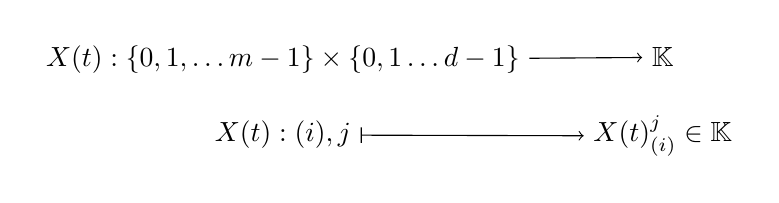
\begin{tikzpicture}
  \matrix (m) [matrix of math nodes, row sep=0.85em, column sep=2em, minimum width=.6em]
  {
	X(t) : \lbrace 0,1,\dots m -1\rbrace \times \lbrace 0 ,1\dots d-1 \rbrace  & \mathbb{K}\\ 
	X(t): (i), j & X(t)_{(i)}^j \in \mathbb{K}\\ 
  }
;
  \path[->]
  (m-1-1) edge node [above] {$$} (m-1-2)
  ;
  \path[|->]
  (m-2-1) edge node [above] {$$} (m-2-2)
  ;
\end{tikzpicture}
\]



For Recurrent Neural Networks (RNN), RNNs have the problem of \emph{exploding gradients}: roughly speaking, 
\[
\text{grad}J \equiv \frac{ \partial J}{ \partial \Theta_I } \sim  ( \Theta_I)^t, \qquad \, t\in \lbrace 0 ,1,\dots T-1 \rbrace
\]
since for each time iteration, a factor of the weight $\Theta$ is multiplied.  

So for the exploding gradient problem, if $\| \Theta_I \| >1$, after $t>1$, the gradient grows; if $\| \Theta_I \| <1$, after $t>1$, gradient goes to $0$, and so long term memories ($t \gg 1$), aren't included: LSTM gradient cannot go to $0$.  

In presenting the definition of Long-Short Term Memory (LSTM), I will present various notation used as even Jozefowicz, Zaremba, and Sutskever \cite{JZS2015} even says different notation is used by practitioners.  They denoted the following:  
\begin{equation}
\begin{aligned}
	& i_t = \tanh{(W_{xi} X_t + W_{hi} h_{t-1} + b_i )}  \\
	& j_t = \text{sigm}{(W_{xj} X_t + W_{hj} h_{t-1} + b_j )}  \\
	& f_t = \text{sigm}{(W_{xf} X_t + W_{hf} h_{t-1} + b_f )}  \\
	& o_t = \tanh{(W_{xo} X_t + W_{ho} h_{t-1} + b_o )}  \\
	& c_t =  c_{t-1}\otimes f_t + i_t \otimes j_t  \\
	& h_t = \tanh{ (c_t)}\otimes o_t  
\end{aligned}
\end{equation}



Jozefowicz, Zaremba, and Sutskever \cite{JZS2015}.  

Bengio, et. al. \cite{GBC2016}



\subsection{How to choose the number of hidden layers and nodes in a neural net}


\part{Convolutional Neural Networks (CNN); CNN, higher-rank tensors}



\subsection*{Convolution}
define \textbf{convolution} of $f,g$ on $\mathbb{R}^n$
\begin{definition}
	\begin{equation}  f* g(x) = \int_{ \mathbb{R}^n } f(x-y)g(y)dy \end{equation}
\end{definition}
Note $f*g = g*f$ by change of variables.  
Now
\[
\begin{gathered}
y(t) = \int_{-\infty}^{\infty}x(\tau)h(t-\tau)d\tau = \int_{-\infty}^{\infty} d\tau \frac{1}{2\pi} \int_{-\pi}^{\pi} \widehat{x}(\omega) e^{i\omega \tau} d\omega h(t-\tau) e^{-i \omega t} e^{-\omega t} = \frac{1}{2\pi} \int_{-\pi}^{\pi} \widehat{x}(\omega) \widehat{h}(\omega) e^{i\omega t} d\omega \\ 
\Longrightarrow \widehat{y}(\omega) = \widehat{x}(\omega) \widehat{h}(\omega)
\end{gathered}
\]
Discrete case: if $f,g$ are \emph{discrete}, i.e. $\begin{aligned} & \quad \\
& f = f(i) \\
& g = g(j) \end{aligned}$, $i,j \in \mathbb{Z}$, then
\[
\int_{-\infty}^{\infty} dy f(x-y)g(y) = \sum_{k=-\infty}^{\infty} f(n-k) g(k) = (f*g)(n)
\]
\section{Images, and generalization of Images as multilinear mappings; Convolution by a filter (stencil $c$)}
Given image of size $L_x \times L_y$, i.e. $(L_x,L_y)\in ( \mathbb{Z}^+)^2$.  An image really is a "designated" or "particular," "fixed" mapping $f$.  
\[
\begin{gathered}
f: \lbrace 0 , \dots L_x- 1\rbrace \times \lbrace 0 \dots L_y-1 \rbrace \to \lbrace 0 \dots 255 \rbrace^4 \\ 
f(x,y) = (f^{(r)}(x,y), f^{(b)}(x,y), f^{(g)}(x,y), f^{(\alpha)}(x,y))
\end{gathered}
\]
Note that $f$ consists of the usual 4 "channels" for rgb color with $\alpha$ denoting "hue."  
Generalize this to the following multilinear mapping:  
with size dimensions $L_1 \times L_2 \times \dots \times L_d, (L_1, L_2 \dots L_d)\in (\mathbb{Z}^+)^d$, 
\begin{equation}
\begin{gathered}
f: \lbrace 0 \dots L_1 - 1 \rbrace \times  \lbrace 0 \dots L_2 - 1 \rbrace \times \dots \times  \lbrace 0 \dots L_d - 1 \rbrace \to \mathbb{K}^C ; \qquad \, C\in \mathbb{Z}^+ , \, \mathbb{K} = \mathbb{R} \text{ or } \mathbb{Z} \\ 
f(x_1,x_2 \dots x_d) = (f^{(1)}(x_1,x_2,\dots x_d), f^{(2)}(x_1,x_2,\dots x_d), \dots f^{(C)}(x_1,x_2,\dots x_d) )
\end{gathered}
\end{equation}
\subsection{Filter (stencil) $c$ }
For the filter (i.e. stencil) $c$, stipulate that $W$'s are odd, (the letter $W$ denote stencil width or filter width).  
\[
\begin{gathered}
	(\nu_x,\nu_y) \in \lbrace 0 \dots W_x-1\rbrace \times \lbrace 0 \dots W_y-1 \rbrace \\
	c : \lbrace 0 , \dots W_x -1\rbrace \times \lbrace 0, \dots W_y-1 \rbrace \to (\mathbb{K})^C  \\
	c(\nu_x,\nu_y) \mapsto c(\nu_x,\nu_y)=(c^{(1)}(\nu_x,\nu_y),c^{(2)}(\nu_x,\nu_y), \dots c^{(C)}(\nu_x,\nu_y)) 
\end{gathered}
\]
In general, 
\begin{equation}
\begin{gathered}
	(\nu_1, \nu_2 \dots \nu_d) \in \lbrace 0 , \dots , W_1-1 \rbrace \times \lbrace 0 , \dots , W_2-1 \rbrace \times \dots \times \lbrace 0 , \dots , W_d-1 \rbrace   \\
	c: \lbrace 0 , \dots W_1 - 1 \rbrace \times \dots \times \lbrace 0 , \dots W_d - 1 \rbrace \to (\mathbb{K})^C  \\
	c(\nu_1 , \nu_2 \dots \nu_d) \mapsto (c^{(1)}(\nu_1 , \dots \nu_d) ,\dots c^{(C)}(\nu_1 \dots \nu_d) )
\end{gathered}
\end{equation}
This filter (stencil) operation, $c\in L(\lbrace 0 \dots W_1 - 1\rbrace \times \dots \times \lbrace 0 ,\dots W_d - 1\rbrace , (\mathbb{K})^C)$, can be isomorphically mapped to a "matrix" or "tensor" of values (but we can only say that it gets mapped into elements in the space of the Cartesian product of vector spaces $(\mathbb{K}^C)^{W_1} \times (\mathbb{K}^C)^{W_2} \times \dots \times (\mathbb{K}^C)^{W_d} \equiv (\mathbb{K}^C)^{W_1 W_2 \dots W_d}$.  We cannot say that it gets mapped to a tensor.  We need to require that this Cartesian product have an equivalence relation be "quotient"-ed out.  For example, if for $(\mathbb{K}^C)^{W_1} \times (\mathbb{K}^C)^{W_2}$, the equivalence relation is of the form $(v_1 + v_2,w) - (v_1,w) - (v_2,w), (v,w_1+w_2)-(v,w_1)-(v,w_2), c(v,w)-(cv,w), c(v,w)-(v,cw)$, $\forall \, v_1,v_2,v \in (\mathbb{K}^C)^{W_1}$, $\forall \, w_1,w_2,w \in (\mathbb{K}^C)^{W_2}$, $c\in \mathbb{K}$.  We must take the quotient according to this equivalence relation.  Then we need to check if this produces the universality property of tensors in the view point of category theory).  
For the sake of notation, since surely $W_i$ is an odd number, then $\forall \, i = 1\dots d$, $W_i = 2h_i + 1$, $h_i \in \mathbb{Z}^+$.  Division with integers yields the "floor."  Keep that mind in the notation of $W_i/2$.  
Then consider the \emph{discrete convolution} $g=c*f$: 
\begin{equation}\label{Eq:DiscreteConvolution}
\begin{gathered}
g^{(\alpha)}(i_1, i_2 \dots i_d) = \sum_{\nu_1=0}^{W_1-1} \sum_{\nu_2=0}^{W_2-1} \dots \sum_{\nu_d=0}^{W_d-1} c^{(\alpha)}(\nu_1 \dots \nu_d ) f^{(\alpha)}(i_1 + \nu_1 - \frac{W_1}{2} , i_2 + \nu_2 - \frac{W_2}{2}, \dots i_d + \nu_d - \frac{W_d}{2}) \qquad \, \forall \, \alpha = 1, 2, \dots C
\end{gathered}
\end{equation}
For the $d=2$ case, 
\[
\begin{gathered}
g^{(\alpha)}(i,j) = \sum_{\nu_1=0}^{W_1-1}\sum_{\nu_2=0}^{W_2-1} c^{(\alpha)}(\nu_1, \nu_2)f^{(\alpha)}(i+\nu_1 - h_1, j +\nu_2 - h_2)
\end{gathered}
\]
Unless there were specified boundary conditions, observe that for $g$, 
\[
\begin{gathered}
h_1 \leq i_1 \leq L_1 - 1 - h_1 \\
h_2 \leq i_2 \leq L_2 - 1 - h_2 \\
\vdots \\ 
h_d \leq i_d \leq L_d - 1 - h_d \\
\end{gathered}
\]
and so observe that unless boundary conditions for $f$ is specified with additional assumptions, 
\begin{equation}
g:\lbrace 0 \dots L_1 -1 - 2h_1 \rbrace \times \lbrace 0 \dots L_2 -1 - 2h_2 \rbrace \times \dots \times \lbrace 0 \dots L_d -1 - 2h_d \rbrace  \to \mathbb{K}^C
\end{equation}
$g$ is "smaller" than $f$ by $\frac{W_1}{2} , \frac{W_2}{2} \dots \frac{W_d}{2}$ in each of dims. $f$ "shrank" to.  
\section{Convolution Axon}
Recall the $l$th axon of the deep neural network (DNN), which consists of the $l-1$th layer, $a^{(l-1)}$ which is the "input" of this axon and the $l$th layer, $a^{(l)}$ the "output" of this axon.  Others call this the "fully-connected layer."  
\begin{equation}
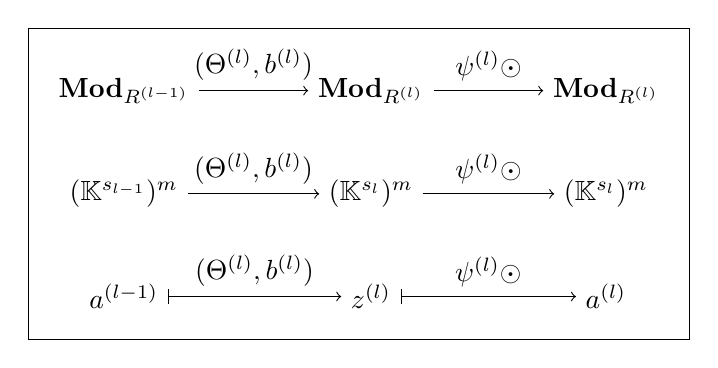
\begin{tikzpicture}[framed]
\matrix (m) [matrix of math nodes, row sep=2.1em, column sep=4em, minimum width=1.5em]
{
	\text{\textbf{Mod}}_{R^{(l-1)}} & \text{\textbf{Mod}}_{R^{(l)}}  & \text{\textbf{Mod}}_{R^{(l)}} \\
	(\mathbb{K}^{s_{l-1}})^m  & (\mathbb{K}^{s_l})^m & ( \mathbb{K}^{s_l})^m  \\ 
	a^{(l-1)}  & z^{(l)} & a^{(l)} \\ 
};
\path[->]
(m-1-1) edge node [above] {$(\Theta^{(l)}, b^{(l)})$} (m-1-2)
(m-1-2) edge node [above] {$ \psi^{(l)} \odot $} (m-1-3)
;
\path[->]
(m-2-1) edge node [above] {$(\Theta^{(l)}, b^{(l)})$} (m-2-2)
(m-2-2) edge node [above] {$ \psi^{(l)} \odot $} (m-2-3)
;
\path[|->]
(m-3-1) edge node [above] {$(\Theta^{(l)}, b^{(l)})$} (m-3-2)
(m-3-2) edge node [above] {$ \psi^{(l)} \odot $} (m-3-3)
;
\end{tikzpicture} 
\end{equation}
with 
\begin{equation}
\begin{gathered}
\begin{gathered}
z^{(l)} := a^{(l-1)} \Theta^{(l)} + b^{(l)} \\
(z^{(l)})_j = (a^{(l+1)})_{\mu} \Theta^{\mu}_{\ \  j}
\end{gathered} \qquad \, \\ 
\text{ e.g. } \Theta^{\mu}_{ \ \  j} \in ( \text{Mat}_{\mathbb{K}}(m,s_{l-1}) )^* \otimes \text{Mat}_{\mathbb{K}}(m,s_l) \cong \text{Mat}_{\mathbb{K}}(s_{l-1},s_l)\\
a^l := \psi^{(l)}(z^{(l)})
\end{gathered}
\end{equation}
Consider again a single "generalized image", as a given element in the space of linear mappings $L\left( \otimes_{i=1}^d \mathbb{K}^{L_i}, \mathbb{K}^C \right)$:  
\begin{equation}
\begin{gathered}
L\left( \otimes_{i=1}^d \mathbb{K}^{L_i}, \mathbb{K}^C \right) \ni \\
\ni (f^{(1)}(x_1,x_2 \dots x_d), f^{(2)}(x_1,x_2 \dots x_d) , \dots f^{(C)}(x_1,x_2 \dots x_d)) \equiv (f^{(1)}),f^{(2)}, \dots f^{(C)} )(x_1,x_2 \dots x_d)
\end{gathered}
\end{equation}
For example, for the case of $d=2$, $C=1$, then we have a \emph{grayscale image} of size dimensions $L_1 \equiv H$, $L_2 \equiv W$ (with $H$, $W$ denoting height and width of an image, respectively).  Then 
\[
L(\mathbb{K}^H \times \mathbb{K}^W, \mathbb{K}) \ni f(x_1,x_2)
\]
e.g. $d=2,C=3$, rgb image (of 3 "channels"):
\[
\begin{gathered}
L(\mathbb{K}^H \times \mathbb{K}^W, \mathbb{K}^3) \ni f(x_1,x_2) = \\
(f^{(r)}(x_1,x_2),f^{(g)}(x_1,x_2),f^{(b)}(x_1,x_2)) = (f^{(r)}, f^{(g)},f^{(b)})(x_1,x_2)
\end{gathered}
\]
Then, as a warm-up, consider the convolution of this single image with a filter (stencil) $c$, as given with Eq. \ref{Eq:DiscreteConvolution}:
\[
\begin{gathered}
g^{(\alpha)}(i_1,i_2 \dots i_d) = \\
= \sum_{\nu_1=0}^{W_1-1} \sum_{\nu_2=0}^{W_2-1} \dots \sum_{\nu_d=0}^{W_d-1} c^{(\alpha)}(\nu_1 \dots \nu_d ) f^{(\alpha)}(i_1 + \nu_1 - \frac{W_1}{2} , i_2 + \nu_2 - \frac{W_2}{2}, \dots i_d + \nu_d - \frac{W_d}{2}) \qquad \, \forall \, \alpha = 1, 2, \dots C
\end{gathered}
\]
But we really want to consider $m$ total samples/examples, concurrently.  Let us, for notation, index these samples/examples by $i_m = 0,1,\dots m-1$.  
Also, consider as a change of notation, where we index the components of $c$ and $f$ to be a subscript, as opposed to being a superscript, before:
\begin{equation}
\begin{gathered}
L(\otimes_{i=1}^d \mathbb{K}^{L_i}, \mathbb{K}^C) \ni \\
\ni (f_1,f_2 \dots f_C)(x_1,x_2 \dots x_d) = (f_1(x_1,x_2 \dots x_d), f_2(x_1\dots x_d), \dots f_C(x_1 \dots x_d))
\end{gathered}
\end{equation}
Then consider the "convolution input layer" to be an element in $ (L(\otimes_{i=1}^d \mathbb{K}^{L_i}, \mathbb{K}^C))^m$: 
\begin{equation}
 (L(\otimes_{i=1}^d \mathbb{K}^{L_i}, \mathbb{K}^C))^m \cong \left( \otimes_{\alpha=1}^C (\otimes_{i=1}^d \mathbb{K}^{L_1}) \right)^m
\end{equation}
Recall again the filter (stencil) $c$, 
\begin{equation}
\begin{gathered}
c: \otimes_{i=1}^d \lbrace 0 ,1,\dots W_i -1\rbrace \to (\mathbb{K})^C  \\
c(\nu_1, \nu_2 ,\dots \nu_d) \mapsto (c_1,c_2, \dots c_C)(\nu_1\dots \nu_d) 
\end{gathered}
\end{equation}
\begin{equation}
\begin{gathered}
f*c = (f*c)_{\alpha}^{(i_m)}(i_1,\dots i_d) = \\
= \sum_{\nu_1=0}^{W_1-1} \sum_{\nu_2=0}^{W_2-1} \dots \sum_{\nu_d=0}^{W_d-1} f_{\alpha}^{(i_m)}(i_1 + \nu_1 - \frac{W_1}{2}, i_2 + \nu_2 - \frac{W_{\alpha}}{2}, \dots i_d + \nu_d - \frac{W_d}{2}) c_{\alpha}(\nu_1 \dots \nu_d)
\end{gathered}
\end{equation}
Consider a bias, $b$, as a $R$-module, 
\[
b \in \left( L (\otimes_{i=1}^d \lbrace 0 ,1, \dots L_i - 1 - 2h_i \rbrace , \mathbb{K}^C) \right)^m
\]
which is "broadcasted" or "copied" $m$ times.  
We can also rewrite this as the following:
\[
\left( \otimes_{i=1}^d ( \mathbb{K}^C)^{L_i - 2h_i} \right)^m  
\]
The Convolution axon (or what others call convolution layer) is in a sense a higher-rank generalization of the DNN axon.  
cf. \href{http://davidstutz.de/wordpress/wp-content/uploads/2014/07/seminar.pdf}{David Stutz's Seminar Report "Understanding Convolutional Neural Networks (2014)}, \url{http://davidstutz.de/wordpress/wp-content/uploads/2014/07/seminar.pdf}



%Consider discrete convolution; $g=c*f$  

%\begin{equation}
%\begin{aligned}
%	g^{(\alpha)}(i_1,i_2 \dots i_d) = \sum_{\nu_1=0}^{W_1-1}\sum_{\nu_2=0}^{W_2-1}  \dots \sum_{\nu_d=0}^{W_d-1}  c^{(\alpha)}(\nu_1 \dots \nu_d )f^{(\alpha)}(i_1 + \nu_1 - \frac{W_1}{2} , i_2 + \nu_2 - \frac{W_2}{2} , \dots i_d + \nu_d - \frac{W_d}{2} )   \\
%\text{ e.g. } g^{(\alpha)}(i,j) = \sum_{\nu_1=0}^{W_1-1} \sum_{\nu_2=0}^{W_2-1}  c^{(\alpha)}( \nu_1 , \nu_2) f^{(\alpha)}(i+\nu_1- h_1 , j+%\nu_2 -h_2)  
%\end{aligned}
%\end{equation}

%Unless there were specified boundary conditions, observe that for $g$, 
%\begin{equation}
%\begin{aligned}
%	& h_1 \leq i_1 \leq L_1 - 1 -h_1 \\ 
%	& h_2 \leq i_2 \leq L_2 - 1 -h_2 \\ 
%	& \vdots 
%	& h_d \leq i_d \leq L_d-1 -h_d 
%\end{aligned}
%\end{equation}
%and so we observe that, unless boundary conditions for $f$ are specified, with additional assumptions, 
%\[
%g: \lbrace 0 \dots L_1 - 1 -2h_1 \rbrace \times \lbrace  0 \dots L_2 - 1 -2h_2 \rbrace \times \dots \times \lbrace 0 , \dots L_d-1 - 2h_d \rbrace \to \mathbb{K}^C
%\]
%$g$ is "smaller" than $f$ by $\frac{W_1}{2} , \frac{W_2}{2} \dots \frac{W_d}{2} $ in each of dims. $f$

\begin{equation}
\begin{gathered}
a_l  = \psi_l \odot ( a_{l-1} * c + b_l ) \text{ with } 
	a_{l-1} \in ( L \left( \bigotimes_{i=1}^d \lbrace 0\dots L_i -1 \rbrace, \mathbb{K}^{C_l-1}  \right) )^m \mapsto ( L \left( \bigotimes_{i=1}^d \lbrace 0\dots L_i -2h_i-1 \rbrace, \mathbb{K}^{C_l-1}  \right) )^m
\end{gathered}
\end{equation}

\subsection{Max-pooling}  

\begin{equation}
\begin{gathered}
	x \in L(\bigotimes_{i=1}^d \lbrace 0 \dots L_i - 1\rbrace ,\mathbb{K} ) \mapsto y \in L(\bigotimes_{i=1}^d \lbrace 0 \dots L_i /P_i - 1\rbrace ,\mathbb{K} )   \text{ where } \\
y(i_1\dots i_d) = \max_{ \substack{ \nu_1 = 0 \dots P_1 - 1 \\ \vdots \\ \nu_d = 0 \dots P_d-1 } } x(i_1 - \nu_1 - \frac{P_1}{2} , \dots i_d - \nu_d - \frac{P_d}{2} )
\end{gathered}
\end{equation}

Here are the necessary (and all) dimensions that have to be provided to define completely the convolution axon, and its respective "name" in \verb|theano|:  

\begin{equation}
\begin{aligned}
\text{ dimensions } & \text{ what theano calls it } \\ 
(C_{l-1}, C_l) \in (\mathbb{Z}^+)^2 & \text{ feature map } \\ 
(W_1 \dots W_d) \in (\mathbb{Z}^+)^d & \text{ filter shape }  \\
(P_1 \dots P_d) \in (\mathbb{Z}^+)^d & \text{ pool size  }  \\ 
(L_1 \dots L_d) \in (\mathbb{Z}^+)^d & \text{ image size }  \\
\end{aligned}
\end{equation}

EY : 20170807 My question is if max-pooling should be its own "layer" or should be done or included with, after, every convolution.  (?,???)

Make a chart of these dimensions and "size dimensions" should be very useful as a sanity check that the dimensions are correct ("shapes" in theano) and to comprehensively and succinctly describe the entire convolution neural network.  I claim that the entire convolution neural network is completely described by these sets of numbers.  For instance, for the example presented in 
\href{http://deeplearning.net/tutorial/lenet.html}{Convolutional Neural Networks (LeNet)} for \verb|theano|, the LeNet is succinctly and entirely described as follows:  
\[
\begin{aligned}
%\begin{tabular}{l c c c c }
& d=2 &  &  & & \\
& l = & 1  \qquad \, &  2 & 3 & \qquad \, 4  \\
& (C_{l-1}, C_l ) \qquad \, & (1,20) \qquad \, & (20,50) & & \\
& (W_1, \dots W_d) & (5,5) \qquad \, &  (5,5) & & \\ 
& (P_1 \dots P_d) & (2,2) \qquad \, & (2,2) & & \\
& (L_1\dots L_d) & (28,28) \qquad \, & (12,12) & & \\ 
& (s_{l-1}, s_l) &                 &              & (50\cdot 4^2, 500) & \qquad \, (500,10)  \\
\end{aligned}
%\end{tabular}
\]
and also these important relations or checks between convolution axons and from a convolution axon to a DNN (i.e. so-called "fully connected layer") can be checked arithmetically, respectively:
\begin{equation}
\begin{gathered}
	L_i^{(l)} = \frac{L_i^{(l-1)} - W_i^{(l-1)} + 1}{ P_i^{(l-1)} } \\ 
s_l = C_{l-1} \prod_{i=1}^d \left( \frac{ L_i^{(l-1)} - W_i^{(l-1)} + 1}{ P_i^{(l-1)} } \right) 
\end{gathered}
\end{equation}

\part{Vision; Computer Vision, 3-dim. Computer Vision, Projections, $\mathbb{R}P^n$}

Cyganek and Siebert (2009) \cite{CySi2009} suggested Hartley and Zisserman (2003) \cite{HaZi2003}

cf. Part I, Camera Geometry and Single View Geometry; Ch. 6 Camera Models; 6.1 Finite cameras of Hartley and Zisserman (2003) \cite{HaZi2003}.  

John Lee (2012) \cite{JLee2012}


We have surjective $\pi$, \\
for $0$ at camera center $C$:  

\begin{equation}
\begin{gathered}
	\mathbb{R}^d \backslash \lbrace 0 \rbrace \xrightarrow{ \pi } \mathbb{R}P^{d-1}  \xrightarrow{ \varphi_d } \\
	(x^1 , \dots x^d) \xmapsto{ \pi } \left[ \left( \frac{x^1}{x^d} \dots \frac{x^{d-1}}{x^d} , 1 \right) \right] \mapsto \left( \frac{x^1}{x^d} \dots \frac{x^{d-1}}{x^d} \right) 
\end{gathered}
\end{equation}

The smooth manifold $\mathbb{R}P^{d-1}$ has an atlas $\mathcal{A}_{\mathbb{R}P^{d-1}}$: 
\begin{equation}
\begin{gathered}
	\mathcal{A}_{\mathbb{R}P^{d-1} } = \lbrace ( U_i , \varphi_i) \rbrace_{i=1}^d \text{ s.t. } \\ 
\begin{gathered}
\begin{aligned}
	& \varphi_i: U_i \to \mathbb{R}^{d-1} , \qquad \, \forall \, i =1 \dots d \\
	& \varphi_i([x^1 \dots x^d]) = \left( \frac{x^1}{x^i} \dots \frac{x^{i-1}}{x^i} , \widehat{1}, \frac{x^{i+1}}{x^i} \dots \frac{x^d}{x^i} \right) 
\end{aligned} \\
\begin{aligned}
	& \varphi_i^{-1} : \mathbb{R}^{d-1} \to U_i \\ 
	& \varphi_i^{-1} (u^1\dots u^{d-1}) = [ (u^1 \dots u^{i-1}, 1, u^i \dots u^{d-1} )]  
\end{aligned}
\end{gathered}
\end{gathered}
\end{equation}
with transition functions
\[
\begin{gathered}
	\begin{aligned}
	& \varphi_j \circ \varphi_i^{-1} : \mathbb{R}^{d-1} \to \mathbb{R}^{d-1} \\ 
	& \varphi_j \circ \varphi_i^{-1} (u^1 \dots u^{d-1}) = \left( \frac{u^1}{u^j} \dots \frac{u^{j-1}}{u^j}  , \frac{u^{j+1}}{u^j}  , \dots \frac{u^{i-1}}{u^j} , \frac{1}{u^j} , \frac{u^i}{u^j}   \dots \frac{u^{d-1}}{u^j}  \right)
\end{aligned}
\end{gathered}
\]

Considering the focal length $f$ of the camera lens, so that the camera focuses the image out at a \emph{focal distance} $f$, by geometry, there's a ratio to be obeyed:
\[
\frac{\alpha}{f} = \frac{y}{z} \Longrightarrow \alpha = \frac{fy}{z}
\]
This is encapsulated in the equivalence relation for $\mathbb{R}P^{d-1}$, namely for so-called \emph{homogeneous coordinates} (Jeffrey Lee (2009)), in that 
\[
\forall \, \lambda \in \mathbb{R} \backslash \lbrace 0 \rbrace , [\lambda x^1 \dots \lambda x^d] = [x^1 \dots x^d] 
\]
and so 
\[
[(x,y,z) ] = [ \left( \frac{x}{z} , \frac{y}{z} , 1 \right) ] = \left[ \left( \frac{fx}{z}, \frac{fy}{z} , f \right) \right]
\]

Center of projection $C \equiv $ \emph{camera center} $\equiv$ \emph{optical center}  \\
\emph{principal axis} or \emph{principal ray} of the camera $\equiv$ line from $C$ perpendicular to image plane.  \\
\emph{principal point} $\equiv $ pt. where principal axis meets image plan.  

\subsubsection{Principal point offset} cf. pp. 155 of Hartley and Zisserman (2003) \cite{HaZi2003}

Consider a point $P_{\text{offset}} = (p^1 \dots p^{d-1}) \in \mathbb{R}^{d-1} = \varphi_d(U_d) \text{ with open } \varphi_d \subset \mathbb{R}P^{d-1}$.  

\begin{equation}
\begin{gathered}
	\mathbb{R}^d \xrightarrow{ \pi } \mathbb{R}P^{d-1} \xrightarrow{ \varphi_d  } \mathbb{R}^{d-1}  \xrightarrow{ f\cdot } \mathbb{R}^{d-1} \xrightarrow{ + P_{\text{offset}} } \mathbb{R}^{d-1} \xrightarrow{ \varphi_d^{-1} } \mathbb{R}P^{d-1}  \\
\begin{gathered}
(x,y,z) \xmapsto{ \pi } [(x,y,z)] = \left[ \left( \frac{x}{z}, \frac{y}{z},1 \right) \right] \xmapsto{ \varphi_d }  \left( \frac{x}{z} , \frac{y}{z} \right) \xmapsto{ f\cdot } \left( \frac{fx}{z} , \frac{fy}{z} \right) \xmapsto{ + P_{\text{offset}} } \left( \frac{fx}{z} + p_x,  \frac{fy}{z} + p_y \right) \xmapsto{ \varphi_d^{-1}} \\
 \xmapsto{ \varphi_d^{-1}} \left[ \left( \frac{fx}{z} + p_x , \frac{fy}{z} + p_y ,1\right) \right] = \left[ (fx+p_xz, fy+p_yz, z) \right]
\end{gathered}
\end{gathered}
\end{equation}

And so harmonize this expression or formulation with that for Hartley and Zisserman (2003) \cite{HaZi2003}.   
\begin{equation}
\begin{gathered}
	\mathbb{R}^3 \xrightarrow{ \varphi_d^{-1} \circ (+P_{\text{offset}} ) \circ (f\cdot) \circ \varphi_3 \circ \pi } \mathbb{R}P^2 \\
(x,y,z) \xmapsto{ \varphi_d^{-1} \circ (+P_{\text{offset}} )\circ (f\cdot) \circ \varphi_3 \circ \pi } [(fx+p_xz, fy+p_yz,z)] \\ 
\left[ \begin{matrix} f & & p_x \\ & f & p_y \\ & & 1 \end{matrix} \right] \left[ \begin{matrix} x \\ y \\ z \end{matrix} \right] = \left[ \begin{matrix} fx+p_x z \\ fy + p_y z \\ z \end{matrix} \right]
\end{gathered}
\end{equation}

\subsubsection{Camera rotation and translation}  cf. pp. 155 of Hartley and Zisserman (2003) \cite{HaZi2003}

We had assumed that $\mathbb{R}^3$ was centered at the camera $C$, camera center.  

In general, consider now this atlas for $\mathbb{R}^3$ (I'll write $\mathbb{R}^d$ to implicitly generalize the space dimensions):  
\[
\mathcal{A}_{\mathbb{R}^3} = \lbrace (\mathbb{R}^3, \varphi_C ) ,(\mathbb{R}^3,\varphi_C) \rbrace
\]
where $(\mathbb{R}^3, \varphi_C )$ are coordinate system centered at $C$, and $(\mathbb{R}^3, \varphi_O )$ is a coordinate system centered at some general point $O$, representing the "world" we're taking a picture of right now.  $\varphi_0 = \varphi^{-1}_0 = 1$.  

Let $C \in \mathbb{R}^d$, $C= (C^1\dots C^d)$ where the camera is, relative to $O$, origin of $\mathbb{R}^d$.  

Then 
\[
\begin{gathered}
\varphi_C \circ \varphi_O^{-1} = \varphi_C \\ 
 \varphi_C \circ \varphi_O^{-1}  (x,y,z) = \varphi_C(x,y,z) \equiv \varphi_C(X) = R(X-C) = R^i_{ \  \  j } (X^j-C^j) = X^i_{\text{(cam)} }
\end{gathered}
\]
with $R$ being a rotation matrix.  

We considered, implicitly, the open sets $U_O$, $U_C$ for the coordinate charts $\varphi_O$, $\varphi_C$ which map a point in $\mathbb{R}^d$ to its coordinates in a coordinate frame \emph{centered} at $O$ or $C$, respectively.  Note that $U_0 = U_C = \mathbb{R}^d$.  And so for the projection, Eq. (6.6), (6.7) of Hartley and Zisserman (2003) \cite{HaZi2003}

\[
\begin{gathered}
\mathbb{R}^d \xrightarrow{ \varphi_C \varphi_O^{-1} } \mathbb{R}^d \xrightarrow{  \varphi_d^{-1} \circ (+P_{\text{offset}} )\circ (f\cdot) \circ \varphi_d \circ \pi } \mathbb{R}P^{d-1}  \\
(x,y,z) \mapsto R((x,y,z) - C) = (x_{\text{(cam)}},y_{\text{(cam)}},z_{\text{(cam)}}) \xmapsto{  \varphi_d^{-1} \circ (+P_{\text{offset}} ) \circ (f\cdot) \circ \varphi_d \circ \pi } \left[ \begin{matrix} f & & p_x \\ & f & p_y \\ & & 1 \end{matrix} \right] \left[ \begin{matrix} x_{\text{(cam)}} \\ y_{\text{(cam)}} \\ z_{\text{(cam)}} \end{matrix} \right] = \left[ \begin{matrix} fx_{\text{(cam)}}+p_x z_{\text{(cam)}} \\ fy_{\text{(cam)}} + p_y z_{\text{(cam)}} \\ z_{\text{(cam)}} \end{matrix} \right] = \\
= \left[ \begin{matrix} fR^1_{ \  \  j}(X^j-C^j)+p_x R^3_{ \  \  j}(X^j-C^j) \\ f R^2_{ \  \  j}(X^j-C^j) + p_y R^3_{ \  \  j}(X^j-C^j) \\ R^3_{ \  \  j}(X^j-C^j) \end{matrix} \right] 
\end{gathered}
\]

\subsubsection{CCD cameras}

$m_x \equiv $ number of pixels per unit distance in image coordinate $x$  \\
$m_y \equiv $ number of pixels per unit distance in image coordinate $y$  

\[
\begin{gathered}
 \mathbb{R}^d = \varphi_C(\mathbb{R}^d) \xrightarrow{  \varphi_d^{-1} \circ (+P_{\text{offset}} )\circ (f\cdot) \circ \varphi_d \circ \pi } \mathbb{R}P^{d-1} \xrightarrow{ \text{diag}(m_x,m_y,1) } \mathbb{R}P^{d-1} \\ 
\varphi_C(X) = X_{\text{(cam)}} \mapsto [(fx_{\text{(cam)}} + p_x z_{\text{(cam)}} , fy_{\text{(cam)}} + p_y z_{\text{(cam)}} , z_{\text{(cam)}} ) ] \mapsto [ (\alpha_x x_{\text{(cam)}} + x_0 z_{\text{(cam)}} , \alpha_y y_{\text{(cam)}} + y_0 z_{\text{(cam)}}, z_{\text{(cam)}} )]
\end{gathered}
\]
with $\begin{aligned} & \quad \\
	& \alpha_x = fm_x \\ 
& \alpha_y = fm_y \end{aligned}$ and $\begin{aligned} & \quad \\
	& x_0 = m_x p_x \\ 
& y_0 = m_y p_y \end{aligned}$

So in general, using composition, 
\begin{equation}
\begin{gathered}
\text{diag}(m_x , m_y , 1) \circ \varphi_d^{-1} \circ ( + P_{\text{offset}} ) \circ (f\cdot)\circ \varphi_d \circ \pi \circ R \equiv \texttt{M} \quad \text{ (pp. 157 of Hartley and Zisserman (2003) \cite{HaZi2003})} = \\
	= \left[ \begin{matrix} \alpha_x & & x_0 \\ & \alpha_y & y_0 \\ & & 1 \end{matrix} \right] R 
\end{gathered}
\end{equation}

\subsubsection{Backprojection of a projective camera; Back-projection of points to rays}  

cf. 6.2.2 Action of a projective camera on points; Back-projection of points to rays of Hartley and Zisserman (2003) \cite{HaZi2003}.  

Given $(u,v) \equiv (u^1 ,u^2) \in \mathbb{R}^{d-1} = \varphi_d(U_d)$ and, given $C \in \varphi_O(\mathbb{R}^d)$ (so $C$ is the camera center with respect to the origin of coordinate chart at $O$), and given focal length $f$, then
\[
\begin{gathered}
\mathbb{R}^{d-1} = \varphi_d(U_d) \xrightarrow{ -P_{\text{offset}} } \mathbb{R}^{d-1}  \xrightarrow{ \frac{1}{f} } \mathbb{R}^{d-1} \xmapsto{ \varphi_d^{-1} } \mathbb{R}P^{d-1} \xrightarrow{ \pi^{-1} } \mathbb{R}^d \\
	(u',v') \xmapsto{ -P_{\text{offset}} } (u,v) = (u'-p_x,v'-p_y)  \xmapsto{ \frac{1}{f} } \left( \frac{u}{f}, \frac{v}{f} \right) \xmapsto{ \varphi_d^{-1} } \left[ \left( \frac{u}{f}, \frac{v}{f},1 \right) \right] = \left[ \left( \frac{uz}{f} , \frac{vz}{f} , z \right) \right] \xrightarrow{ \pi^{-1} } \left( \frac{uz}{f}, \frac{vz}{f} , z \right)  \\
\Longrightarrow  \left[ \begin{matrix} \frac{z}{f} & 0 \\  & \frac{z}{f} \\ & \end{matrix} \right] \left[ \begin{matrix} u \\ v \end{matrix} \right] + z \left[ \begin{matrix}  0 \\ 0 \\ 1 \end{matrix} \right] = (x,y,z)
\end{gathered}
\]
and so $z$, the "depth" of pt. $X\in \mathbb{R}^3 = \mathbb{R}^d$ must be given.  



\subsubsection{Pl\"{u}cker coordinates}  

Let $x,y \in L \subset \mathbb{R}^d$ (e.g. $d=3$), $x\neq y$.  \\
Define $d:= x-y \in \mathbb{R}^d$.  \\
"moment" $m:= x\wedge y = x^i e_i \wedge y^j e_j = x^i y^j e_i \wedge e_j = x^i y^j \epsilon_{ijk} e_k \in \mathbb{R}^d$.  

So $d\cdot m =0$, since $(x-y)\cdot (x\wedge y) =0$.  

Consider 
\[
[(d^1\dots d^d,m^1 \dots m^d)] = [(d^1,d^2,d^3,m^1,m^2,m^3)] \in \mathbb{R}P^5
\]
In a $\mathbb{R}P^3 = \mathbb{R}P^d$, let $L\subset \mathbb{R}P^^3$, let $x,y \in \mathbb{R}P^3$, $x\neq y$.  

\textbf{Pl\"{u}cker coordinates} $p_{ij} = x_i y_j - x_j y_i $, $i,j=0,1,2,3$.  

So $p_{ij} = [(p_{01}, p_{02}, p_{03}, p_{23}, p_{31}, p_{12}) ] \in \mathbb{R}P^5$.  

Another way to write this:  
\[
\begin{gathered}
	M:= \left[ \begin{matrix} x_0 & y_0 \\ x_1 & y_1 \\ x_2 & y_2 \\ x_3 & y_3 \end{matrix} \right] \\
 p_{ij}  =\text{det}(M_i*, M_{j*} )
\end{gathered}
\]
For $x_0=1$, 
\begin{equation}
\begin{gathered}
d=(p_{01},p_{02}, p_{03}) \\
m = (p_{23}, p_{31},p_{12}) \end{gathered}
\end{equation}

Given $p_{ij} = [(d,m)]$, 
\begin{equation}
0 = d\times q - m, \qquad \, \forall \, q \in \text{ line } L_0
\end{equation}
cf. \url{http://orb.olin.edu/plucker.pdf}



\url{http://ags.cs.uni-kl.de/fileadmin/inf_ags/3dcv-ws11-12/3DCV_WS11-12_lec05.pdf}  

Prof. D. Stricker.  3D Computer Vision, Winter Semester 2011-2012.  

\subsection{Fundamental matrix, $F$}

Fundamental matrix $F$ is a rank $2=d-1$ matrix.  

\subsubsection{Examples with 2 cameras; Fundamental matrix $F$}

cf. Example I of \url{http://ags.cs.uni-kl.de/fileadmin/inf_ags/3dcv-ws11-12/3DCV_WS11-12_lec05.pdf}  

Compute the fundamental matrix of a parallel camera stereo rig.  

$C=0=\varphi_0(0) \in \mathbb{R}^3 = \varphi_0(\mathbb{R}^3) $; \quad \, $R=1$.  $P_{\text{offset}}=0$.  $f=f'$  \\
$C'=(t_x,0,0) \in \mathbb{R}^3 = \varphi_0(\mathbb{R}^3)$, $R=1$.  $P_{\text{offset}}' = 0$.  

\[
\begin{gathered}
	\mathbb{R}^d = \varphi_0(\mathbb{R}^3) \xrightarrow{ \varphi_d^{-1} f \circ \varphi_d \circ \pi } \mathbb{R}P^{d-1} \\ 
 X \mapsto \varphi_d^{-1}(f\left( \frac{x}{z}, \frac{y}{z} \right) ) = \left[ \left( \frac{fx}{z}, \frac{fy}{z},1 \right) \right] = [ (fx,fy,z) ] = \\
= KX=\left[ \begin{matrix} f & & \\ & f & \\ & & 1 \end{matrix} \right] X
\end{gathered}
\]

For the other image point on the other camera, 
\[
\begin{gathered}
	\mathbb{R}^d = \varphi_0(\mathbb{R}^3) \xrightarrow{ \varphi_d^{-1} f \circ \varphi_d \circ \pi (-C)} \mathbb{R}P^{d-1} \\ 
X \mapsto \varphi_d^{-1} \left( f\left( \frac{x-t_x}{z} , \frac{y}{z} \right) \right) = \left[ \left( \frac{f(x-t_x )}{z} , \frac{fy}{z},1\right) \right] = [(f(x-t_x), fy,z) ] = K(X-C')
\end{gathered}
\]

Plugging into the formula for $F$:  
\[
\begin{gathered}
	F= ((K')^{-1})^T(\mathbf{t} \times (RK^{-1}) ) = 
\left[ \begin{matrix} 1/f & & \\ & 1/f & \\ & & 1 \end{matrix} \right] \left[ \begin{matrix} & & \\ & & -t_x \\ & t_x & \end{matrix} \right] \left[ \begin{matrix} 1/f & & \\ & 1/f & \\ & & 1 \end{matrix} \right] = \left[ \begin{matrix} 1/f & & \\ & 1/f & \\ & & 1 \end{matrix} \right] \left[ \begin{matrix} & & \\ & & -t_x \\ & \frac{t_x}{f} & \end{matrix} \right] = \left[ \begin{matrix} & & \\ & & -t_x/f \\ & \frac{t_x}{f} & \end{matrix} \right] = \frac{t_x}{f} \left[ \begin{matrix} & & \\ & & -1 \\ & 1 & \end{matrix} \right]
\end{gathered}
\]
with $R=1$ in this case. 

Since $F$ homgeneous, $F\sim \left[ \begin{matrix} & & \\ & & -1 \\ & 1 & \end{matrix} \right]$.  

\[
\begin{gathered}
v^T F u \equiv (u')^T Fu \equiv (x')^T Fx = \left( \frac{ f(x-t_x)}{z}, \frac{fy}{z} ,1 \right) \left[ \begin{matrix} & & \\ & & -t_x \\ & t_x & \end{matrix} \right] \left[ \begin{matrix} \frac{fx}{z} \\ \frac{fy}{z} \\ 1 \end{matrix} \right] = \left( \frac{ f(x-t_x)}{z} , \frac{fy}{z} ,1\right) \left[ \begin{matrix} 0 \\ -t_x \\ \frac{fy}{z} t_x \end{matrix} \right] = 0 
\end{gathered}
\]




\part{Support Vector Machines (SVM)}

The clearest and most mathematically rigorous (and satisfying) introductory exposition on support vector machines (SVM) comes out of a Bachelor's thesis from Nowak (2008) \cite{Nowa2008}.  There is a lot of material that tries to talk about SVM, but the implementation either boils down to showing how to turn the crank on a black-box solution, or is too verbose without saying anything substantial.  I'll include references and links of the material I looked at and didn't find as helpful as Nowak (2008) \cite{Nowa2008}.  

\href{https://d18ky98rnyall9.cloudfront.net/_246c2a4e4c249f94c895f607ea1e6407_Lecture12.pdf?Expires=1490227200&Signature=VxrCShNSKNcYN9~2eHC~IQoQv11wIyqVGEMWVtaycFoimayg-XnGkJaBR4s~aIGf3nq~ck-W5ow4WM0-3vLuxfSkmhQflZH4Bx5fVo2w3R~bldnsJc91Bq-w27KZTw-Xanct~Cn7RnT0ViPlGYeUBmmrSoXAer5IZyPVdmbChzY_&Key-Pair-Id=APKAJLTNE6QMUY6HBC5A}{Lecture12 pdf slides for Ng's Machine Learning Intro. for coursera}

\href{http://www.cs.columbia.edu/~kathy/cs4701/documents/jason_svm_tutorial.pdf}{Support Vector Machine
(and Statistical Learning Theory) Tutorial by Jason Weston, NEC Labs America}

\href{https://en.wikipedia.org/wiki/Support_vector_machine}{Wikipedia page for Support Vector Machine}

\href{https://arxiv.org/pdf/1610.09932.pdf}{Support Vector Machines and Generalisation in HEP} Not much real generalization going on here other than a recap of literally what's exactly in Shawe-Taylor and Cristianini (2000) \cite{STCr2000}.  

\url{https://www.cs.cornell.edu/people/tj/publications/joachims_99a.pdf}

\section{From linear classifier as a hyperplane, (big) margin, to linear support vector machine (SVM), and Lagrangian dual (i.e. conjugate variables, conjugate momenta)}

Intuitively, we seek to find a boundary line that'll draw a line that separates the data points into distinct $K$ (usually $K=2$) classes to classify the data points.  Then, this boundary line will help to predict what class a new data point would fall into, be classified to be.  For a linear model, i.e. ``linear discriminator'', what we're trying to do is \\

find
\[
\theta \in \mathbb{R}^d \backslash \lbrace 0 \rbrace ,\, b\in \mathbb{R}
\]
s.t.
\begin{equation}
  y^{(i)}(\langle \theta,x^{(i)} \rangle + b) - 1 \geq 0 \qquad\, \forall \, i = 1, \dots, m 
\end{equation}
where $\| \theta \|$ is minimal.  It is minimal because, since the distance between 2 hyperplanes,
\[
\langle \theta, x\rangle - b = \pm 1 \qquad \, (\text{defining equations for hyperplanes})
\]
is
\[
\frac{2}{\|\theta\|} \qquad \, (\text{distance between 2 hyperplanes})
\]
Thus, we want the ``margins'', that distance between hyperplanes separating the input data points, to be as big as possible, and so we want $\|\theta\|$ small.

Consider this cost functional, called ``Lagrangian'', that we want to minimize:
\begin{equation}\label{Eq:costLagrangian}
  \mathcal{L}((\theta,b),\lambda) = \frac{1}{2} \| \theta\|^2 - \sum_{j=1}^m \lambda_i y^{(i)}(\langle \theta, x^{(i)} \rangle - b - 1)   =  \frac{1}{2} \| \theta\|^2 - \sum_{j=1}^m \lambda_i y^{(i)}(\langle \theta, x^{(i)} \rangle - b) +\sum_{i=1}^m \lambda_i 
  \end{equation}
Note that
\begin{equation}
f_0((\theta,b)) := \frac{1}{2} \| \theta \|^2 (\text{objective function (slightly modified)})
\end{equation}
is the objective function, what we want to minimize.

The KKT condition tells us that $(\theta,b)$ makes $\mathcal{L}$ a minimum for a certain $\lambda$:
\begin{equation}\label{Eq:partialsL}
  \begin{aligned}
    & \frac{ \partial \mathcal{L}}{ \partial \theta_j} = 0 = \theta_j - \sum_{i=1}^m \lambda_i y^{(i)} x_j^{(i)} \\ 
    & \frac{ \partial \mathcal{L}}{ \partial b} = 0 = -\sum_{i=1}^m \lambda_i y^{(i)}
    \end{aligned}
  \end{equation}
Note that this step in taking the partial derivatives of $\mathcal{L}$ in Eq. \ref{Eq:partialsL} is analogous to the construction/computation of dual ``conjugate'' variables, conjugate momentum, in physics.  

Notice then that
\begin{equation}
  \begin{gathered} \frac{1}{2} \| \theta \|^2 = \frac{1}{2} \sum_{i,j=1}^m \lambda_i \lambda_j y^{(i)} y^{(j)} \langle x^{(i)}, x^{(j)} \rangle \text{ and } \\
    \sum_{i=1}^m \lambda_i y^{(i)} (\langle \theta, x^{(i)} \rangle -b ) =\sum_{i=1}^m \lambda_i y^{(i)} (\sum_{j=1}^m \lambda_j y^{(j)} \langle x^{(j)}, x^{(i)} \rangle )
    \end{gathered}
  \end{equation}
\begin{equation}
\Longrightarrow \mathcal{L}((\theta,b),\lambda) = -\frac{1}{2} \sum_{i,j=1}^m \lambda_i \lambda_j y^{(i)} y^{(j)} \langle x^{(i)} , x^{(j)} \rangle + \sum_{i=1}^m \lambda_i
\end{equation}

\section{So-called ``Kernel trick''; feature space is a Hilbert space}

The so-called ``feature space'' $F$ is a Hilbert space $H$, $\Phi:\mathbb{R}^d \to H$, equipped with inner product
\begin{equation}
\langle \Phi(x), \Phi(y) \rangle = K(x,y)
  \end{equation}
with $K: \mathbb{K}^d\times \mathbb{K}^d \to \mathbb{K}^K$ being called the kernel function.  Recall that the feature space $F$ had been introduced to represent the process of preprocessing input data $X$.  For example, given a single input data example, $X=(X_1,\dots, X_d)\in \mathbb{R}^d$, maybe we'd want to consider polynomial features, linear combinations of various orders of monomials $X_iX_j$ or $X_i^2 X_j$, and so on.  Then $\Phi$ represents the map from $X$ to all these features.

The essense of the kernel trick is this: the explicit form of $\Phi$ need not be known, nor even the space $H$.  Only the kernal function $K$ form needs to be guessed at.  

And so even if we now have to modify our Eq. \ref{Eq:costLagrangian} to account for this preprocessing map $\Phi$, applied first to our training data $x^{(i)} \equiv X^{(i)}$ (Novak's notation vs. Andrew Ng's notation), we essentially still have the same form, formally.

Keep in mind the whole point of this nonlinear preprocessing map $\Phi$ - we want to keep the linear discrimination procedure with the weight, or parameter $\theta$, and intercept $b$, being this linear model on the feature space (Hilbert space) $F$.  We're linear in $F$.  But we're nonlinear in the input data $X=\lbrace X^{(1)},\dots X^{(m)}\rbrace$.

So,
\begin{equation}
  \begin{gathered}
    \mathcal{L}((\theta,b),\lambda) = \frac{1}{2} \| \theta\|^2 - \sum_{j=1}^m \lambda_i y^{(i)}(\langle \theta, \Phi(x^{(i)}) \rangle - b - 1)   =  \frac{1}{2} \| \theta\|^2 - \sum_{j=1}^m \lambda_i y^{(i)}(\langle \theta, x^{(i)} \rangle - b) +\sum_{i=1}^m \lambda_i \text{ and so } \\
    \frac{ \partial \mathcal{L}}{ \partial \theta_j} = 0 = \theta_j - \sum_{i=1}^m \lambda_i y^{(i)} \Phi(x)^{(i)}_j \\
    \Longrightarrow \mathcal{L}((\theta,b),\lambda) = -\frac{1}{2} \sum_{i,j=1}^m \lambda_i \lambda_j y^{(i)} y^{(j)} \langle \Phi(x^{(i)}) , \Phi(x^{(j)}) \rangle + \sum_{i=1}^m \lambda_i
    \end{gathered}
  \end{equation}

\subsection{Dealing with Errors, (non-negative) slack variables, dealing with not-necessarily perfectly separable data}

First, loosen the strict constraint $y^{(i)}(\langle \theta,x^{(i)} \rangle - b) \geq 1$ by introducing \emph{non-negative} slack variables $\xi_i$, $i=1\dots m$,
\begin{equation}
  y^{(i)}(\langle \theta, x^{(i)} \rangle - b) \geq 1 - \xi_i, \qquad \, \forall \, i = 1,2, \dots m 
\end{equation}
Simply add $\xi$ to the objective function to implement penalty (for ``too much slack''):
\begin{equation}
  f_0(\theta,b,\mathbf{\xi}) = \frac{1}{2} \| \theta \|^2 + C\sum_{i=1}^m \xi_i
  \end{equation}



So then the total Lagrangian becomes
\begin{equation}
  \mathcal{L}(\theta,b,\xi,\lambda,\mu) = \frac{1}{2} \| \theta \|^2 + C\sum_{i=1}^m \xi_i - \sum_{i=1}^m \lambda_i (y^{(i)}(\langle \theta,x^{(i)} \rangle -b)-1 +\xi_i ) - \sum_{i=1}^m \mu_i \xi_i
\end{equation}
where the constraint is turned into a Lagrange-multiplier type relation:
\begin{equation}
\xi_i \geq 0 \Longrightarrow \mu_i(\xi_i - 0) \qquad \, \forall \, i =1,\dots m 
\end{equation}
$-\mu_i\xi_i$ is indeed a valid cost (penalty) functional (if $\xi_i  <0$, $-\mu_i\xi_i >0$, and there's more penalty as $\xi_i$ gets more negative.  Note that I understood this cost or penalty accounting, given an \emph{inequality constraint}, from reading notes from here, \href{http://www.pitt.edu/~jrclass/opt/notes4.pdf}.   








\section{Dual Formulation}

\begin{equation}\label{Eq:DualFormulation}
\begin{gathered}
  \text{min}. \qquad \, W(\lambda) = -\sum_{i=1}^m \lambda_i +\frac{1}{2} \sum_{i,j=1}^m \lambda_i \lambda_j y^{(i)} y^{(j)} K(x^{(i)},x^{(j)}) \\
  \text{ s.t. } \begin{aligned} & \quad \\
    & \sum_{i=1}^m \lambda_i y^{(i)} = 0  \\
    & 0 \leq \lambda_i \leq C \end{aligned}
  \end{gathered}
  \end{equation}

At this point, Eq. \ref{Eq:DualFormulation} is what I could consider the ``theoretical gold'' version.  Further modification of this formulation are really to efficiently implement this on the computer (or microprocessor!).  But the schemes should respect this ``gold'' version and compute what this is and say.  

\subsection{Implementation}

Wotao Yin's notes had a terse, but to-the-point, survey/summary of optimization, in particular nonlinear optimization with inequality constraints, for his courses \href{http://www.math.ucla.edu/~wotaoyin/math273a/slides/Lec6_NLP_w_inequality_constraints_273a_2015_f.pdf}{273a} and \href{http://www.math.ucla.edu/~wotaoyin/math164/slides/wotao_yin_optimization_lec13_algorithms_for_constrained_optimization.pdf}{Math 164, Algorithms for constrained optimization}.  In both course notes, the material is ``taken from the textbook Chong-Zak, 4th. Ed.''  So we'll refer to Chong and Zak (2013) \cite{ChZa2013}.   

From Ch. 22 ``Algorithms for Constrained Optimization'', 2nd. Ed., from pp. 439, Sec. 22.2 Projections, consider $\Omega \subset \mathbb{R}^d$, \[
\Omega = \lbrace \mathbf{x} | l_i \leq x_i \leq u_i , \, i = 1\dots d\rbrace
\]

Let $\Pi \equiv $ projection operator.  Define the above case as such:

\[
\begin{gathered}
  \forall \, \mathbf{x} \in \mathbb{R}^d, \, y := \Pi[x] \in \mathbb{R}^d \\ 
  y_i \equiv \begin{cases} u_i & \text{ if } x_i > u_i \\
    x_i & \text{ if } l_i \leq x_i \leq u_i \\
    l_i & \text{ if } x_i < l_i \end{cases}
  \end{gathered}
\]







\subsubsection{Projected Gradient descent}.

Implement $\sum_{i=0}^m \lambda_i y^{(i)} = 0$, consider the orthogonal projector matrix (operator)
\begin{equation}
  \mathbf{P} := \mathbf{1}_{\mathbb{R}^d} - A^T(AA^T)^{-1}A
  \end{equation}





If $m=1$, then
\[
\text{Proj}_{\Omega}(\mathbf{y}) = \mathbf{y} - \frac{\mathbf{a}_1^T \mathbf{y} - b}{ \| \mathbf{a}_1 \|^2 } \mathbf{a}_1
\]

If $m>1$, then
\[
\text{Proj}_{\Omega}(\mathbf{y}) = (1_{\mathbb{R}^d} - A^T(AA^T)^{-1}A)\mathbf{y}+A^T(AA^T)^{-1}\mathbf{b}
\]

For the linear (but it's an equality) constraint
\[
\sum_{i=1}^m \lambda_iy^{(i)} = 0 
\]
so
\begin{equation}
  \mathbf{P}_{\sum_{i=1}^m\lambda_iy^{(i)} = 0 }(\mathbf{y}) = \left( \mathbf{y} - \frac{ \sum_{i=1}^m y^{(i)} (\mathbf{y})_i }{ \sum_{i=1}^m (y^{(i)})^2 } (y^{(i)})\mathbf{e}_i \right)
  \end{equation}


\href{http://drona.csa.iisc.ernet.in/~e0270/Jan-2015/Tutorials/lecture-notes-3.pdf}{Narasimhan's Optimization Tutorial 3, Projected Gradient Descent, Duality} had some concrete pseudocode for the projected gradient descent \cite{Nara2015}.

In summary,
\begin{equation}
\begin{gathered}
  \begin{gathered}
    \text{ we seek to minimize } \\
    W(\lambda) = - \sum_{i=1}^m \lambda_i + \frac{1}{2} \sum_{i,j=1}^m \lambda_i \lambda_j y^{(i)} y^{(j)} K(X^{(i)},X^{(j)}) \qquad \, \forall \, i=1,2,\dots m 
  \end{gathered} \\
  \text{  by iterating $t=0,1,\dots $, as such: } \\
  \begin{aligned}
    & \lambda_i'(t+1):=\lambda_i(t) - \alpha \text{grad}{ W(\lambda) } \\ 
    & \lambda''_i(t+1):= \mathbf{P}_{\sum_{i=1}^m \lambda_i y^{(i)} = 0 }( \lambda_i'(t+1)) \\ 
    & \lambda_i(t+1) := \Pi_{0\leq \lambda_i \leq C}(\lambda_i''(t+1))
    \end{aligned}
\end{gathered}
\end{equation}
where
\begin{equation}
\begin{aligned}
& \mathbf{P}_{\sum_{i=1}^m \lambda_i y^{(i)} = 0 }( \lambda_i'(t+1)) = \lambda_i'(t+1) - \frac{ \sum_{i=1}^m y^{(i)}\lambda_i'(t+1) }{ \sum_{i=1}^m (y^{(i)})^2 } y^{(i)} \\ 
  & \Pi_{0\leq \lambda_i \leq C}(\lambda_i''(t+1)) = \begin{cases} C & \text{ if } \lambda_i''(t+1) > C \\
    \lambda_i''(t+1) & \text{ if } 0 \leq \lambda_i''(t+1) \leq C \\
    0 & \text{ if } \lambda_i'(t+1) <0 \end{cases}
\end{aligned}
\end{equation}

\subsubsection{Computing $b$, the intercept, with a good algebra tip: multiply both sides by the denominator}

Bishop (2007) \cite{Bish2007}, on pp. 330 of Ch. 7, Sparse Kernel Machines,  gave a very good (it resolved possible numerical instabilities) prescription on how to compute the intercept $b$, given $\lambda$, which would then give us the function that can make predictions $\widehat{y}$ on input data example $X^{(i)} \in X$.  It's worth expounding upon here.  

For any support vector (Bishop called it a support vector; what I think it's equivalent to is that we've trained on our training set $(X,y)^{\text{train}}$, and this is 1 of the training examples) $X^{(i)}$, $i=1\dots m$,
\begin{equation}
  y^{(i)}f(X^{(i)}) =1
  \end{equation}.  Then using
\begin{equation}
\begin{gathered}
  f(x):=\sum_{i=1}^m y^{(i)} \lambda_i^* K(X^{(i)},x) + b \\
  \Longrightarrow y^{(i)} \left( \sum_{j=1}^m y^{(j)} \lambda_j^* K(X^{(j)},X^{(i)} ) + b \right) = 1
  \end{gathered}
  \end{equation}
Although we can solve this equation for $b$ with algebra/arithmetic for our arbitrarily chosen support vector, it's numerically more stable to 1st. multiply through by $y^{(i)}$, using $(y^{(i)})^2 =1$, and then averaging over all support vectors.
\begin{equation}
  \begin{gathered}
    \sum_{j=1}^m y^{(j)}\lambda_j^* K(X^{(j)},X^{(i)}) +b = y^{(i)} \\
    \Longrightarrow b= \frac{1}{m} \left( \sum_{i=1}^m y^{(i)} - \sum_{i,j=1}^m y^{(j)} \lambda_j^* K(X^{(j)}, X^{(i)}) \right)
    \end{gathered}
  \end{equation}

\subsubsection{Prediction (with SVM)}

\begin{equation}
  \begin{aligned}
    & \widehat{y}(X) = \sum_{i=1}^m y^{(i)} \lambda_i^* K(X^{(i)}, X) + b^* \\ 
    & \widehat{y}:\mathbb{R}^d \to \lbrace 0 ,1 , \dots , K-1 \rbrace
    \end{aligned}
  \end{equation}


Clarke, Fokoue, and Zhang (2009) \cite{CFZ2009}



\section{Support Vector Machines (SVM) natively implemented in theano, entirely on the GPU with the CUDA backend, with constrained gradient descent}

\subsection{Executive Summary}

I implemented SVM natively in theano, and can run entirely on the GPU(s) (through the CUDA C/C++ backend).  Solving the \emph{constrained optimization} problem to train a SVM here used \emph{parallel reduce} algorithms; in fact a parallel reduce nested in side a parallel reduce.  The work complexity achieved in this case should be of $O(2\log{m})$ where $m$ is the total number of training examples, as opposed to $O(m^2)$ for Quadratic Programming (QP), such as Sequential Minimal Optimization (SMO).  Training on the same data set for vehicles as previous work for C/C++ library \verb|libsvm| that uses SMO, \verb|SVM_parallel| (what I call the described implementation here) achieves an accuracy of 95.1\% on test data, as opposed to 87.8\% for \verb|libsvm|.  What I'd like to do in the future is to train and test on larger datasets ($m>10000$) to test \verb|SVM_parallel| for its promising scalability, and to implement it as the outer layer of a deep neural network (DNN) for ``Deep SVM''.  

\subsection{Motivations and Introductions}\label{Sec:MotivationsIntroductions}

Support Vector Machines (SVM) can be used for (binary) classification in supervised learning on labeled data, being able to learn non-linear, higher-dimensional features and to predict a boundary line or discriminator between classes, through the so-called \emph{kernel trick}, which is really to presume a higher-dimensional Hilbert space to represent feature space $\mathcal{F}$ (i.e. $\mathcal{F}$ is a Hilbert space).

I considered the proposition of having, as a final, outer ``layer,'' of a deep neural network (DNN) to be a support vector machine.  Could it outperform the same DNN with a sigmoid or softmax function at the final layer?

To my knowledge, there was not a native implementation of SVM on theano, a Python framework for deep learning/DNNs.  Being that I sought to speed up learning/computation on the GPU(s) through the theano CUDA backend, it would seem to defeat the GPU speedup advantages if from the very last layer, a large global memory transfer had to occur from the GPU (with the last DNN layer), to a host CPU, \emph{serial}, implementation of SVM.  Global memory transfers are prohibitive expensive, for latency, i.e. time-wise, between host CPU and GPUs.\cite{CS344}    

The outline/plan/highlights for this (short) paper is as follows: in
\begin{itemize}
\item \ref{Sec:ConciseMathReview}, I review or summarize points in the theory for SVM, give derivations, etc., in which (this has all been done before; I sought to give a concise review)
  \begin{itemize}
\item \ref{SubSec:Hyperplanes}, I recap basic, elementary concepts motivating the linear discriminator concept and what hyperplanes are, and how they're defined by a \emph{linear} function
\item \ref{SubSec:MarginsLagrangian} - I continue to review and present derivations for the \emph{Lagrangian}, a Lagrange multiplier problem, we want to minimize, and apply the usual Karush-Kuhn-Tucker (KKT) condition to make progress in deriving the constrained optimization problem we seek to solve,
\item \ref{SubSec:Kerneltrick} kernel trick, with the feature space $\mathcal{F}$ as a Hilbert space, \ref{SubSec:slackvars} slack variables to deal with non-perfectly-separable data, and more derivation that was done before, but made explicitly here
\end{itemize}
\item \ref{Sec:DualFormulation}, the \emph{constrained optimization} problem we wish to solve for SVM
\item \ref{Sec:ConstrainedOptimization}, I translate how our constrained optimization problem is to be solved with \emph{projected gradient descent} or ``constrained gradient descent'' (as the projection operators enforce constraint equalities and inequalities).  As noted, this method/algorithm was chosen to utilize the (very useful) \verb|grad| method in the \verb|theano| software package.

  The Eqns. \ref{Eq:DualFormulationW}, \ref{Eq:ProjectionOpsAlgo} at the end of \ref{SubSec:ProjectedGradDescent} is the crux of the training method considered in this paper and code for SVM and was directly referred to when implemented in code.  
  \begin{itemize}
  \item I also show how to compute, in a numerically stable manner, the intercept $b$, after $\lambda_i$ Lagrange multipliers are found, and how to compute predictions $\widehat{y}$, in \ref{SubSec:binterceptcompute}, \ref{SubSec:Predictioncompute}
  \end{itemize}
  \item \ref{Sec:ConstrainedGradDescImplementation} the \emph{constrained gradient descent} to solve our constrained optimization problem is implemented and I detail its implementation using software package \verb|theano|, and especially its CUDA backend, so to run solely on the \emph{GPU}.  I give the rationale in deploying this constrained gradient descent as opposed to the Sequential Minimal Optimization (SMO) usually used in the predominant SVM software package (in C/C++) \verb|libsvm|.  Noteworthy, I also show that \textbf{work complexity goes from $O(m^2)$ to $O(2\log(m))$}.  
\item \ref{SubSec:Code} briefly tells where the code is made available and the 1-to-1 correspondence between the code and mathematical formulation.  I also note that \emph{novel use of theano's reduce within reduce}.  
\item \ref{SubSec:ResultsSampleDatasets} has \emph{results} that I try to compare with sample datasets used previously, that I've trained as quickly as possible.  Look here for the results; better yet, feel free to try the code and jupyter notebook and share benchmarks.\footnote{\href{https://github.com/ernestyalumni/MLgrabbag/blob/master/ML/SVM.py}{github:ernestyalumni/MLgrabbag/ML}, \href{https://github.com/ernestyalumni/MLgrabbag/blob/master/SVM_theano.ipynb}{github:ernestyalumni/MLgrabbag SVM theano.ipynb}}
\end{itemize}

\subsection{Concise Mathematical Review/Summary of the theory for SVM}\label{Sec:ConciseMathReview}

\subsubsection{Hyperplanes and distances to motivate the linear discriminator concept; Support Vector Machine name}\label{SubSec:Hyperplanes}

I'll recap basic, elementary concepts, from Clarke, Fokoue, and Zhang (2009) \cite{CFZ2009}, that motivate the concept of a linear discriminator classifying input data $X$.

Consider $\theta\in \mathbb{R}^d$, and a linear function $y$,
\begin{equation}\label{Eq:yforhyperplane}
\begin{aligned}
& y:\mathbb{R}^d \to \mathbb{R} \\
  & y(x) := \langle \theta,x \rangle +b 
  \end{aligned}
\end{equation}
Consider a ``level set'' at real number value $c\in \mathbb{R}$, $H_c(\theta,b)$:
\begin{equation}\label{Eq:H_cHyperplane}
H_c(\theta,b):=\lbrace x|y(x) = \langle \theta,x\rangle +b =c \rbrace 
  \end{equation}
where $\text{dim}H_c(\theta,b)=d-1$ is a \emph{hyperplane}.

$\theta\in \mathbb{R}^d$ is the normal vector to this hyperplane, since,
\[
\begin{gathered}
  \forall \, x^{(i)}, x^{(j)} \in H_c(\theta,b), \text{ then } \\
  \langle \theta, x^{(i)} \rangle + b = c = \langle \theta , x^{(j)}\rangle + b \Longrightarrow \langle \theta, x^{(i)} - x^{(j)} \rangle = 0 
  \end{gathered}
\]
and since $x^{(i)} - x^{(j)} \in TH_c(\theta,b)$, i.e. $x^{(i)} - x^{(j)}$ belongs in the tangent space to $H_c(\theta,b)$, $TH_c(\theta,b)$, then $\theta$, in general, is normal to the hyperplane ($\langle \theta, x^{(i)} - x^{(j)} \rangle =0$).

Given $z\in \mathbb{R}^d$, what is the distance from $z$ to this hyperplane $H_c(\theta,b)$, $d(z,H_c(\theta,b))$?  Consider $z* = z+t\theta\in H_c(\theta,b)$.  Then
\[
\begin{gathered}
  \langle \theta, z^*\rangle + b=c = \langle \theta,z \rangle + t\langle \theta, \theta\rangle + b = c \Longrightarrow t=\frac{ c-b-\langle \theta,z\rangle }{ \| \theta \|^2}  \\
  \text{ and so }
  d(z,H_c(\theta,b)) = \| t\theta \| = \frac{ | \langle \theta , z \rangle +b- c | }{\| \theta \| } 
  \end{gathered}
\]
Thus, for the perpendicular distance between 2 parallel hyperplanes, $H_c(\theta,b)$, $H_{c'}(\theta,b)$, can be found: choose a pt. from $H_c(\theta,b)$, without loss of generality, s.t. $z=\left( \frac{c-b}{\theta_1},0 , \dots 0 \right)$, so that
\[
\langle \theta,z \rangle + b=c \Longrightarrow \theta_1z^1 = c-b
\]
Then
\begin{equation}
d(H_c(\theta,b),H_{c'}(\theta,b)) = \frac{  | \langle \theta,z \rangle +b-c' | }{ \| \theta \| } = \frac{ | c-b+b-c' | }{ \| \theta \| } = \frac{ |c-c' | }{ \| \theta \| }
  \end{equation}

Given an input (data) domain $\mathcal{X}\subseteq \mathbb{R}^d$, for the case of binary classification, with total number of classes $K=2$, we can consider representing the outcomes $y$ for each input data example, $X \in \mathbb{R}^d$, in 2 ways:
\begin{equation}
  y\in \lbrace -1 , 1 \rbrace \text{ \textbf{or } } y\in \lbrace 0,1 \rbrace \text{ for } y \in \lbrace 0 , 1, \dots K-1\rbrace \, (K=2)
  \end{equation}
What ends up happening is that the distance between 2 hyperplanes, $c=-1,c'=1$ vs. $c=0,c'=1$, respectively, changes, as $d(H_c(\theta,b),H_{c'}(\theta,b)) = \frac{ |c-c' | }{ \| \theta \| }$, but its absolute value doesn't matter.  What matters is the form of $y:\mathbb{R}^d \to \mathbb{R}$, of Eq. \ref{Eq:yforhyperplane} which defines the hyperplane in Eq. \ref{Eq:H_cHyperplane}, notably in $\theta,b$.  The lesson is to \emph{be consistent with what the value of $y$ is to define what class $X$ belongs to}.  For instance, Bishop (2007) \cite{Bish2007} and Clarke, Fokoue, and Zhang (2009) \cite{CFZ2009} chooses to consider $y\in \lbrace - 1, 1 \rbrace, \, \forall \, X$ and I'll do the same here.

The name ``support vectors'' seems to come from this intuitive notion: $\theta \in \mathbb{R}^d$,$b$ are determined from $m$ input data examples $X^{(i)} \in \mathbb{R}^d$, $\forall \, i = 1, 2, \dots d$, and $\forall \, i$, the corresponding class label $y\in \mathbb{Z}$.  $\forall \, X^{(i)} \in \mathbb{R}^d$, imagine attaching normal vectors of the form $t\theta$, $t\in\mathbb{R}$ that extend out to the respective hyperplane, determined by $y^{(i)}$.  These imagined vectors ``support'' the respective hyperplane.  

An important takeaway is that the equation defining the hyperplane $H_c{(\theta,b)}$ in Eq. \ref{Eq:H_cHyperplane} is \emph{linear}.  

\subsubsection{Margins, cost functional or ``Lagrangian'', dual formulation}\label{SubSec:MarginsLagrangian}

With output, outcome $y\in \lbrace - 1, 1 \rbrace, \, \forall \, X$ input data example, the distance between the 2 hyperplanes, which are level sets of $c=-1,c'=1$, is
\[
\frac{2}{\| \theta \| }
\]
The method of SVM seeks to maximize this distance, also known as ``margin'', to make margins as big as possible.  

Clearly, this is equivalent to minimizing $\frac{1}{2} \| \theta \|^2$, with $\frac{1}{2}$ multiplication factor chosen, without loss of generality, to make taking derivatives of $\theta$ easier.

But we also have the following constraints.  We want to have a ``margin'' of $\frac{2}{\|\theta\|}$ between the hyperplanes that'll separate the input data examples $X^{(i)}$, $\forall \, i =1,2,\dots m$, for different classes, in this binary classification class, of those with $y^{(i)} \in \lbrace -1, 1\rbrace$, and so those $X^{(i)}$'s will ``fall far away'' from this ``margin'' and remain within its corresponding hyperplane $H_{c'=1}(\theta,b)$ or $H_{c=1}(\theta,b)$, thus defining these inequalities:
\begin{equation}\label{Eq:ineqconstraints}
  y^{(i)}(\langle \theta,x^{(i)} \rangle + b) - 1 \geq 0 \qquad\, \forall \, i = 1, \dots, m 
\end{equation}
So we want to find 
\[
\theta \in \mathbb{R}^d \backslash \lbrace 0 \rbrace ,\, b\in \mathbb{R}
\]
s.t.
\[
y^{(i)}(\langle \theta,x^{(i)} \rangle + b) - 1 \geq 0 \qquad\, \forall \, i = 1, \dots, m
\]
where $\frac{2}{\| \theta \|}$ is maximized, or equivalently, defining the so-called \emph{objective function} $f_{\theta}(\theta,b)$, minimize $f_{\theta}(\theta,b)$:
\begin{equation}
f_{\theta}(\theta,b) := \frac{1}{2} \| \theta \|^2 \qquad \, (\text{objective function})
\end{equation}

Consider then this cost functional, also known as the ``Lagrangian'', which we want to \emph{minimize}.  
\begin{equation}\label{Eq:costLagrangianL}
  \mathcal{L}((\theta,b),\lambda) = \frac{1}{2} \| \theta\|^2 - \sum_{j=1}^m \lambda_i y^{(i)}(\langle \theta, x^{(i)} \rangle + b - 1)   =  \frac{1}{2} \| \theta\|^2 - \sum_{j=1}^m \lambda_i y^{(i)}(\langle \theta, x^{(i)} \rangle + b) +\sum_{i=1}^m \lambda_i 
  \end{equation}
Of note, we introduced \emph{Lagrangian multipliers} $\lambda_i$, $\forall i \in 1,2\dots m$, $\lambda_i \in \mathbb{R}$, to account for each of the constraints given in Eq. \ref{Eq:ineqconstraints}.  

The Karush-Kuhn-Tucker (KKT) condition tells us that $(\theta,b)$ makes $\mathcal{L}$ a minimum for a certain $\lambda$ (and that these $\lambda_i$'s exist), and that these relations hold:\cite{Nowa2008}, \cite{ChZa2013}:
\begin{equation}\label{Eq:partialsL}
  \begin{aligned}
    & \frac{ \partial \mathcal{L}}{ \partial \theta_j} = 0 = \theta_j - \sum_{i=1}^m \lambda_i y^{(i)} x_j^{(i)} \qquad \, j=1,2\dots d \\ 
    & \frac{ \partial \mathcal{L}}{ \partial b} = 0 = -\sum_{i=1}^m \lambda_i y^{(i)}
    \end{aligned}
\end{equation}
and
\begin{equation}
\lambda_i \geq 0 \qquad\, \forall \, i = 1, 2, \dots m
\end{equation},
\begin{equation}\label{Eq:KKTcond3}
\sum_{j=1}^m\lambda_iy^{(i)}(\langle \theta,x^{(i)}\rangle ) +b-1) = 0 
\end{equation}
$\forall \, i =1,2,\dots m$, we want input data example $X^{(i)}$ to be ``far away'' from the boundary line, or, i.e. to give enough ``margin'' from the other class's hyperplane, and so in general, $(\langle \theta,x^{(i)}\rangle ) -b-1)$ will be non-zero in Eq. \ref{Eq:KKTcond3}.  So this condition is equivalently
\begin{equation}
\sum_{j=1}^m\lambda_iy^{(i)} =0
  \end{equation}

It's interesting to see that the step in taking the partial derivatives of $\mathcal{L}$ in Eq. \ref{Eq:partialsL} is analogous to the construction/computation of dual ``conjugate'' variables, conjugate momentum, in physics.  

Notice then that
\begin{equation}
  \begin{gathered} \frac{1}{2} \| \theta \|^2 = \frac{1}{2} \sum_{i,j=1}^m \lambda_i \lambda_j y^{(i)} y^{(j)} \langle x^{(i)}, x^{(j)} \rangle \text{ and } \\
    \sum_{i=1}^m \lambda_i y^{(i)} (\langle \theta, x^{(i)} \rangle +b ) =\sum_{i=1}^m \lambda_i y^{(i)} (\sum_{j=1}^m \lambda_j y^{(j)} \langle x^{(j)}, x^{(i)} \rangle )
    \end{gathered}
  \end{equation}
\begin{equation}
\Longrightarrow \mathcal{L}((\theta,b),\lambda) = -\frac{1}{2} \sum_{i,j=1}^m \lambda_i \lambda_j y^{(i)} y^{(j)} \langle x^{(i)} , x^{(j)} \rangle + \sum_{i=1}^m \lambda_i
\end{equation}


\subsection{So-called ``Kernel trick''; feature space is a Hilbert space}\label{SubSec:Kerneltrick}

The so-called ``feature space'' $\mathcal{F}$ is a Hilbert space $\mathcal{H}$, $\Phi:\mathbb{R}^d \to \mathcal{H}$, equipped with inner product
\begin{equation}
\langle \Phi(x), \Phi(y) \rangle = K(x,y)
  \end{equation}
with $K: \mathbb{K}^d\times \mathbb{K}^d \to \mathbb{K}^K$ being called the kernel function.  Recall that the feature space $\mathcal{F}$ had been introduced to represent the process of preprocessing input data $X$.  For example, given a single input data example, $X=(X_1,\dots, X_d)\in \mathbb{R}^d$, maybe we'd want to consider polynomial features, linear combinations of various orders of monomials $X_iX_j$ or $X_i^2 X_j$, and so on.  Then $\Phi$ represents the map from $X$ to all these features.

As both a pedantic remark and academic question, I had denoted $\mathbb{K}$ to be, in general, a \emph{field} - (very familiar) examples of fields are $\mathbb{K}=\mathbb{R}, \mathbb{C}, \mathbb{Z}$, the real numbers, complex numbers, integers, respectively.  Many times, input data that we receive could take on discrete values, meaning $X^{(i)} \in \mathbb{Z}$.  Would there be issues, in proving existence, continuity, and differentiability, throughout derivations for these SVM algorithms, if the underlying field $\mathbb{K}$ is not the real number line $\mathbb{R}$?

Nevertheless, the essense of the kernel trick is this: the explicit form of $\Phi$ need \emph{not be known}, nor even the space $\mathcal{H}$.  Only the kernal function $K$ form needs to be guessed at.  

And so even if we now have to modify our Eq. \ref{Eq:costLagrangianL} to account for this preprocessing map $\Phi$, applied first to our training data $X^{(i)}$, we essentially still have the same form, formally.

Keep in mind the whole point of this nonlinear preprocessing map $\Phi$ - we want to keep the linear discrimination procedure with the weight, or parameter $\theta$, and intercept $b$, being this linear model on the feature space (Hilbert space) $F$.  We're \emph{linear} in $\mathcal{F}$.  But we're \emph{nonlinear} in the input data $X=\lbrace X^{(1)},\dots X^{(m)}\rbrace$'s domain.

So,
\begin{equation}
  \begin{gathered}
    \mathcal{L}((\theta,b),\lambda) = \frac{1}{2} \| \theta\|^2 - \sum_{j=1}^m \lambda_i y^{(i)}(\langle \theta, \Phi(x^{(i)}) \rangle + b - 1)   =  \frac{1}{2} \| \theta\|^2 - \sum_{j=1}^m \lambda_i y^{(i)}(\langle \theta, x^{(i)} \rangle + b) +\sum_{i=1}^m \lambda_i \text{ and so } \\
    \frac{ \partial \mathcal{L}}{ \partial \theta_j} = 0 = \theta_j - \sum_{i=1}^m \lambda_i y^{(i)} \Phi(x)^{(i)}_j \\
    \Longrightarrow \mathcal{L}((\theta,b),\lambda) = -\frac{1}{2} \sum_{i,j=1}^m \lambda_i \lambda_j y^{(i)} y^{(j)} \langle \Phi(x^{(i)}) , \Phi(x^{(j)}) \rangle + \sum_{i=1}^m \lambda_i = \mathcal{L}(X,y,\lambda)
    \end{gathered}
  \end{equation}
Note that we'll now want to \emph{maximize} this dual formulation $\mathcal{L}(X,y,\lambda)$.  


\subsubsection{Dealing with Errors, (non-negative) slack variables, dealing with not-necessarily perfectly separable data}\label{SubSec:slackvars}

First, ``loosen the strict constraint'' $y^{(i)}(\langle \theta,x^{(i)} \rangle + b) \geq 1$ by introducing \emph{non-negative} slack variables $\xi_i$, $i=1\dots m$,
\begin{equation}
  y^{(i)}(\langle \theta, x^{(i)} \rangle - b) \geq 1 - \xi_i, \qquad \, \forall \, i = 1,2, \dots m 
\end{equation}
Simply add $\xi$ to the objective function to implement penalty (for ``too much slack''), with a ``regularization'' constant $C$ (in analogy to regularization in the linear regression or logistic regression classifier methods):
\begin{equation}
  f_0(\theta,b,\mathbf{\xi}) = \frac{1}{2} \| \theta \|^2 + C\sum_{i=1}^m \xi_i
  \end{equation}

cf. Andrew Ng's Support Vector Machines Large Margin Intuition, The mathematics behind large margin classification (optional), Kernels II,   

\subsubsection{SVM parameters}  

$C ( = \frac{1}{\lambda})$.  Large $C$: lower bias, high variance.  (small $\lambda$) \\
Small $C$: Higher bias, low variance (large $\lambda$)

For 
\[
\exp{ \left( - \frac{ \| x - l^{(i) } \|^2 }{ 2\sigma^2 } \right) }
\]

$\sigma^2$.  Large $\sigma^2$: Features $f_i$ vary more smoothly.  Higher bias, lower variance.  

Small $\sigma^2$.  Features $f_i  $ vary less smoothly.  

Lower bias, higher variance.  




So then the total Lagrangian becomes
\begin{equation}
  \mathcal{L}(\theta,b,\xi,\lambda,\mu) = \frac{1}{2} \| \theta \|^2 + C\sum_{i=1}^m \xi_i - \sum_{i=1}^m \lambda_i (y^{(i)}(\langle \theta,x^{(i)} \rangle +b)-1 +\xi_i ) - \sum_{i=1}^m \mu_i \xi_i
\end{equation}
where the constraint is turned into a Lagrange-multiplier type relation:
\begin{equation}
\xi_i \geq 0 \Longrightarrow \mu_i(\xi_i - 0) \qquad \, \forall \, i =1,\dots m 
\end{equation}
$-\mu_i\xi_i$ is indeed a valid cost (penalty) functional (if $\xi_i  <0$, $-\mu_i\xi_i >0$, and there's more penalty as $\xi_i$ gets more negative.  I understood this cost or penalty accounting, given an \emph{inequality constraint}, from reading notes from here, \url{http://www.pitt.edu/~jrclass/opt/notes4.pdf}).

If we ``turn the crank'' and take partial derivatives of $\mathcal{L}$, with respect to $\xi_i$, finding its ``conjugate momentum dual'', we'll actually see that $\mathcal{L}$ has \emph{no} dependence on $\xi_i$:
\begin{equation}
\begin{gathered} \begin{gathered}
  \frac{ \partial \mathcal{L}}{ \partial \xi_i} = C-\lambda_i -\mu_i = 0 \\ 
  \text{ since } \begin{aligned} & \quad \\
    C - \lambda_i = \mu_i \\
    \mu_i \geq 0 \text{ is given } \end{aligned} \qquad \, \Longrightarrow C \geq \lambda_i 
  \end{gathered}
  \Longrightarrow \\
  \mathcal{L}(\theta,b,\xi,\lambda,\mu) = \frac{1}{2} \| \theta \|^2 - \sum_{i=1}^m \lambda_i(y^{(i)} ( \langle \theta, \Phi(x^{(i)})\rangle ) + \sum_{i=1}^m \lambda_i  = \mathcal{L}((\theta,b),\lambda)
  \end{gathered}
  \end{equation}
$\xi,\mu$ no longer appear in the dual Lagrangian, $\mathcal{L}(X,y,\lambda)$, which we want to \emph{maximize}, nor in the so-called ``primal'' Lagrangian, $\mathcal{L}((\theta,b),\lambda)$.  

%which we'll now denote $W=W(\lambda)$, nor in Lagrangian $\mathcal{L}((\theta,b),\lambda)$.  

\subsection{Dual Formulation}\label{Sec:DualFormulation}

Denoting $W(\lambda):= -\mathcal{L}(X,y,\lambda)$, 

\begin{equation}\label{Eq:DualFormulation}
\boxed{ \begin{gathered}
  \text{minimize}. \qquad \, W(\lambda) = -\sum_{i=1}^m \lambda_i +\frac{1}{2} \sum_{i,j=1}^m \lambda_i \lambda_j y^{(i)} y^{(j)} K(x^{(i)},x^{(j)}) \\
  \text{ s.t. } \begin{aligned} & \quad \\
    & \sum_{i=1}^m \lambda_i y^{(i)} = 0  \\
    & 0 \leq \lambda_i \leq C \qquad \, \forall \, i = 1,2 \dots m \end{aligned}
  \end{gathered} }
  \end{equation}

At this point, Eq. \ref{Eq:DualFormulation} is what I could consider the ``theoretical gold'' version.  Further modification of this formulation are really to efficiently implement this on the computer (or microprocessor!).  But the schemes should respect this ``gold'' version and compute what this is and say.  

\subsection{Constrained Optimization}\label{Sec:ConstrainedOptimization}

Wotao Yin's notes had a terse, but to-the-point, survey/summary of optimization, in particular nonlinear optimization with inequality constraints, for his courses \href{http://www.math.ucla.edu/~wotaoyin/math273a/slides/Lec6_NLP_w_inequality_constraints_273a_2015_f.pdf}{273a} and \href{http://www.math.ucla.edu/~wotaoyin/math164/slides/wotao_yin_optimization_lec13_algorithms_for_constrained_optimization.pdf}{Math 164, Algorithms for constrained optimization}.  In both course notes, the material is ``taken from the textbook Chong-Zak, 4th. Ed.''  So we'll refer to Chong and Zak (2013) \cite{ChZa2013}.   

From Ch. 22 ``Algorithms for Constrained Optimization'', 2nd. Ed., pp. 439, Sec. 22.2 ``Projections'', consider $\Omega \subset \mathbb{R}^d$, with \[
\Omega = \lbrace \mathbf{x} | l_i \leq x_i \leq u_i , \, i = 1\dots d\rbrace
\]

Let us denote $\Pi \equiv $ projection operator.  Let us mathematically formulate how projection operator $\Pi$ maps a point $\mathbf{x} \in \mathbb{R}^d$ onto the subset $\Omega \subset \mathbb{R}^d$ defined above: 
\begin{equation}\label{Eq:ProjectionOperatorInequalities}
\begin{gathered}
  \forall \, \mathbf{x} \in \mathbb{R}^d, \, y := \Pi[x] \in \mathbb{R}^d \\ 
  y_i \equiv \begin{cases} u_i & \text{ if } x_i > u_i \\
    x_i & \text{ if } l_i \leq x_i \leq u_i \\
    l_i & \text{ if } x_i < l_i \end{cases}
  \end{gathered}
\end{equation}

\subsubsection{Projected Gradient descent}\label{SubSec:ProjectedGradDescent}

We want to minimize $W(\lambda)$ in Eq. \ref{Eq:DualFormulation}.  The software package \verb|theano| provides the graph-generating method \verb|grad|, which automatically computes the symbolic gradient of a scalar-valued function of symbolic (theano) variables.  This \verb|grad| has been very useful for automating the computation of the so-called ``back-propagation'' step of machine learning/deep learning.

We would like to reuse this useful theano method for SVM.  Therefore I sought out a solution to our constrained optimization problem that'll involve computing gradients at each iteration, but subject to our constraint equality and inequalities.

We already know how to deal with constraint \emph{inequalities} via the projection operator in Eq. \ref{Eq:ProjectionOperatorInequalities}.  And note that this can be simply implemented in Python/theano with a \verb|if/else| statement(s) and \verb|theano.tensor.switch|, respectively.  

To implement the constraint \emph{equality}, $\sum_{i=0}^m \lambda_i y^{(i)} = 0$, consider the orthogonal projector matrix (operator)
\begin{equation}
  \mathbf{P} := \mathbf{1}_{\mathbb{R}^d} - A^T(AA^T)^{-1}A 
  \end{equation}
with $A$ being a transformation from $\mathbb{R}^d$ to $\mathbb{R}^m$, i.e. $A: \mathbb{R}^d \to \mathbb{R}^m$, and where $Ax = b$ is the constraint equality (written in its most general form) \cite{ChZa2013}.  

So for where $\Omega = \lbrace X | AX = b \rbrace$, if $m=1$, then
\[
\text{Proj}_{\Omega}(\mathbf{y}) = \mathbf{y} - \frac{\mathbf{a}_1^T \mathbf{y} - b}{ \| \mathbf{a}_1 \|^2 } \mathbf{a}_1
\]

If $m>1$, then
\[
\text{Proj}_{\Omega}(\mathbf{y}) = (1_{\mathbb{R}^d} - A^T(AA^T)^{-1}A)\mathbf{y}+A^T(AA^T)^{-1}\mathbf{b}
\]

For the linear (equality) constraint
\[
\sum_{i=1}^m \lambda_iy^{(i)} = 0 
\]
we have
\begin{equation}
  \mathbf{P}_{\sum_{i=1}^m\lambda_iy^{(i)} = 0 }(\mathbf{y}) = \left( \mathbf{y} - \frac{ \sum_{i=1}^m y^{(i)} (\mathbf{y})_i }{ \sum_{i=1}^m (y^{(i)})^2 } (y^{(i)})\mathbf{e}_i \right)
  \end{equation}


In summary,
\begin{equation}\label{Eq:DualFormulationW}
\boxed{ \begin{gathered}
  \begin{gathered}
    \text{ we seek to minimize } \\
    W(\lambda) = - \sum_{i=1}^m \lambda_i + \frac{1}{2} \sum_{i,j=1}^m \lambda_i \lambda_j y^{(i)} y^{(j)} K(X^{(i)},X^{(j)}) 
  \end{gathered} \\
  \text{  by iterating $t=0,1,\dots $, as such: } \\
  \begin{aligned}
    & \lambda_i'(t+1):=\lambda_i(t) - \alpha \text{grad}{ W(\lambda) } \\ 
    & \lambda''_i(t+1):= \mathbf{P}_{\sum_{i=1}^m \lambda_i y^{(i)} = 0 }( \lambda_i'(t+1)) \\ 
    & \lambda_i(t+1) := \Pi_{0\leq \lambda_i \leq C}(\lambda_i''(t+1))
    \end{aligned}
\end{gathered} }
\end{equation}
where
\begin{equation}\label{Eq:ProjectionOpsAlgo}
\boxed{ \begin{aligned}
& \mathbf{P}_{\sum_{i=1}^m \lambda_i y^{(i)} = 0 }( \lambda_i'(t+1)) = \lambda_i'(t+1) - \frac{ \sum_{i=1}^m y^{(i)}\lambda_i'(t+1) }{ \sum_{i=1}^m (y^{(i)})^2 } y^{(i)} \\ 
  & \Pi_{0\leq \lambda_i \leq C}(\lambda_i''(t+1)) = \begin{cases} C & \text{ if } \lambda_i''(t+1) > C \\
    \lambda_i''(t+1) & \text{ if } 0 \leq \lambda_i''(t+1) \leq C \\
    0 & \text{ if } \lambda_i'(t+1) <0 \end{cases}
\end{aligned} }
\end{equation}
The $\alpha$ parameter is the analogue to the \emph{learning rate} of gradient descent and will need to be tuned.  

\subsubsection{Computing $b$, the intercept, with a good algebra tip: multiply both sides by the denominator}\label{SubSec:binterceptcompute}

Bishop (2007) \cite{Bish2007}, on pp. 330 of Ch. 7, Sparse Kernel Machines,  gave a very good (it resolved possible numerical instabilities) prescription on how to compute the intercept $b$, given $\lambda$, which would then give us the function that can make predictions $\widehat{y}$ on input data example $X^{(i)} \in X$.  It's worth expounding upon here.  

For any support vector (Bishop called it a support vector; what I think it's equivalent to is that we've trained on our training set $(X,y)^{\text{train}}$, and this is 1 of the training examples) $X^{(i)}$, $i=1\dots m$,
\begin{equation}
  y^{(i)}f(X^{(i)}) =1
  \end{equation}.  Then using
\begin{equation}
\begin{gathered}
  f(x):=\sum_{i=1}^m y^{(i)} \lambda_i^* K(X^{(i)},x) + b \\
  \Longrightarrow y^{(i)} \left( \sum_{j=1}^m y^{(j)} \lambda_j^* K(X^{(j)},X^{(i)} ) + b \right) = 1
  \end{gathered}
  \end{equation}
Although we can solve this equation for $b$ with algebra/arithmetic for our arbitrarily chosen support vector, it's numerically more stable to 1st. multiply through by $y^{(i)}$, using $(y^{(i)})^2 =1$, and then averaging over all support vectors.
\begin{equation}\label{Eq:bintercept}
  \begin{gathered}
    \sum_{j=1}^m y^{(j)}\lambda_j^* K(X^{(j)},X^{(i)}) +b = y^{(i)} \\
    \Longrightarrow b= \frac{1}{m} \left( \sum_{i=1}^m y^{(i)} - \sum_{i,j=1}^m y^{(j)} \lambda_j^* K(X^{(j)}, X^{(i)}) \right)
    \end{gathered}
  \end{equation}

\subsubsection{Prediction (with SVM)} \label{SubSec:Predictioncompute}
Compute predictions with this formula: \cite{CFZ2009}
\begin{equation}\label{Eq:predictyhat}
  \begin{aligned}
    & \widehat{y}(X) = \sum_{i=1}^m y^{(i)} \lambda_i^* K(X^{(i)}, X) + b^* \\ 
    & \widehat{y}:\mathbb{R}^d \to \lbrace 0 ,1 , \dots , K-1 \rbrace \quad \, (\text{with $K=2$ for binary classification})
    \end{aligned}
  \end{equation}





\subsection{Constrained Gradient Descent (Implementation)}\label{Sec:ConstrainedGradDescImplementation}

From Eqns. \ref{Eq:DualFormulationW}, \ref{Eq:ProjectionOpsAlgo}, with the algorithm or iterative, computational steps that we should take mathematically formulated (clearly), I had sought out to implement these steps using \verb|theano| and on the GPU, in the hopes of speeding up computation and developing a method that can scale with $m$ input data examples.  

Take a look at this double summation term in Eqn. \ref{Eq:DualFormulationW} for $W(\lambda)$:
\begin{equation}\label{Eq:doublesumf_1}
f_1(\lambda) := \frac{1}{2} \sum_{i,j=1}^m \lambda_i \lambda_j y^{(i)} y^{(j)} K(X^{(i)},X^{(j)}) = \frac{1}{2} \sum_{i=1}^m\sum_{j=1}^m \lambda_i y^{(i)} K(X^{(i)},X^{(j)}) \lambda_j y^{(j)} = (\mathbf{q}^{(i)})^T K(X^{(i)},X^{(j)}) \mathbf{q}^{(j)}
\end{equation}
Quadratic programming (denoted ``QP'' in computer science literature) is essentially trying to put the calculation of double sums, such as the above, into quadratic form, as in the very last equality.  Techniques for efficient calculation, on the CPU, of this quadratic form, after reformulation of the original problem, make up QP.

The prevailing software package used for SVM, written in C/C++, that also underlies SVM module for sci-kit learn (\verb|sklearn|) \cite{Pedr2011} is \verb|libsvm| \cite{ChLi2011}.  \verb|libsvm| employs the method of Sequential Minimal Optimization (SMO) \cite{Pla1998}.  The main advantage of SMO is that only 2 $\lambda_i$'s, Lagrange multipliers, are considered in the working set at each stage in time and the optimal solution is computed analytically at this point.

For instance, suppose we are considering 2 Lagrange multipliers $\lambda_1$ and $\lambda_2$.  We first compute the optimal value changing $\lambda_2$ only.  Then, using the inequality constraints $0 \leq \lambda_1,\lambda_2\leq C$, and equality constraint $\sum_{i=1}^m \lambda_iy^{(i)} =0$ (but adapted to the fact that we're only changing 2 $\lambda_i$'s), we can analytically compute the other $\lambda_1$.

The (serial) computation in C/C++ of this analytical problem at this single step for SMO is fast.  However, for the fitting for large data sets (large $m$), the fit time complexity is more than quadratic with the number of examples $m$, which makes it difficult to scale to datasets of more than a couple of 10000 examples ($m>10000$) \footnote{\href{http://scikit-learn.org/stable/modules/generated/sklearn.svm.SVC.html\#sklearn.svm.SVC}{sklearn.svm.SVC}} \cite{Pedr2011}.  

Instead, I considered the idea behind \emph{All-pairs $N$-body} algorithm of Nyland, Harris, and Prins (2007) in Ch. 31 of \textbf{GPU Gems 3} \cite{Ngu2007}.  It was also explained in Udacity's CS344 with Owens and Luebke \cite{CS344} \footnote{\href{https://classroom.udacity.com/courses/cs344/lessons/116611037/concepts/1198442170923\#}{Quiz: All Pairs $N$-Body}}.  

Look again at Eq. \ref{Eq:doublesumf_1}, $f_1$, which clearly requires $m^2$ fetches, or reads, for $\lambda_i \lambda_j y^{(i)} y^{(j)} K(X^{(i)},X^{(j)})$ term and $m^2$ computations, for each $(i,j)$ pairs (and there are $m^2$ total pairs).  It could also help to imagine a $m\times m$ matrix:

%\begin{tikzpicture}
%\matrix[matrix of nodes]{
%$i=1,j=1$ & $i=1,j=2 $  \\% 
%};
%\end{tikzpicture}

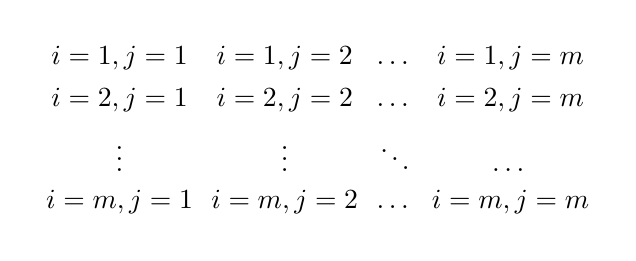
\begin{tikzpicture}
\matrix[matrix of nodes]{
$i=1,j=1$ & $i=1,j=2$ & $\dots$ & $i=1,j=m$ \\    $i=2,j=1$ & $i=2,j=2$ & $\dots$ & $i=2,j=m$ \\    $\vdots$ & $\vdots$ & $\ddots$ & $\dots$ \\ $i=m,j=1$ & $i=m,j=2$ & $\dots$ & $i=m,j=m$ \\% <- Without this %, there would be a trailing "1" in the copied text
};
\end{tikzpicture}

and observing that $\forall \, i=1,2,\dots m$, we're doing $m$ computations for $j$ and needing to fetch $m$ values for each $\lambda_j$, $y_j$, $X^{(j)}$, and so on.

Consider this computation: for a given, single $i\in \lbrace 1,2,\dots m\rbrace$, define 
\begin{equation}
f_{1i}(\lambda) := \frac{1}{2} \sum_{j=1}^m \lambda_j y^{(j)} K(X^{(i)},X^{(j)})
\end{equation}
For this step, we'll only need to do $m$ fetches for the $\lambda_j,y^{(j)},X^{(j)}$ values, and $X^{(i)}$ value will be fetched once.  As this is a summation over a potentially large vector ($m$ can be big), this looks like a good case/candidate for the usage of parallel \emph{reduce} algorithm.  The work complexity of parallel reduce is $O(\log{m})$ \cite{CS344}\footnote{\href{https://youtu.be/tSgVVVTe5KQ}{Step Complexity of Parallel Reduce - Intro to Parallel Programming, Udacity}}.  Theano has an implementation of reduce in \verb|theano.reduce|.

Once all $m$ $f_{1i}$'s are obtained, for $i=1,2,\dots m$, then parallel reduce can be used again (especially if $m$ is large!).  Also, empirically, I found that using \verb|theano.reduce| again helped to circumvent the problem of the maximum recursion limit for Python \footnote{\href{https://github.com/Theano/Theano/issues/689}{max recusion limit \#689}}, which is inherent with Python (cf. \verb|import sys  sys.getrecursionlimit()|).  In practice, above about 10000 recursions, the Python script fails with run-time errors.

Nevertheless, in this second (parallel) reduce step, we are doing
\[
f_1 = \sum_{i=1}^m \lambda_i y^{(i)} f_{1i}(\lambda)
\]
with $m$ fetches of values for $\lambda_i, y^{(i)}$.  The work complexity here for this reduce step is again $O(\log(m))$

Thus, we are doing, for 2 (parallel) reduces, $2m$ fetches (or reads), for each $\lambda_i$ or $y^{(i)}$ or $X^{(i)}$.

The total work complexity is $O(2\log(m))$.  

Likewise, for the computation of the intercept $b$ in Eqn. \ref{Eq:bintercept}, after minimizing $W(\lambda)$ by varying $\lambda$, I also employed parallel reduce via \verb|theano.reduce| (but only once for the single sum) and for the prediction step for $\widehat{y}$ in Eq. \ref{Eq:predictyhat}

\subsubsection{Code (theano/Python script), jupyter notebook accompanying code}\label{SubSec:Code}

SVM is implemented as described above, in particular Eqns. \ref{Eq:DualFormulationW}, \ref{Eq:ProjectionOpsAlgo}, in the Python class \verb|SVM_parallel|.  The default kernel function $K:\mathbb{R}^d\times \mathbb{R}^d \to \mathbb{R}^d$ is the radial basis function, which takes the form of a gaussian, is first implemented and I can implement other kernel functions easily, as a Python function object and Python class member, in the future.

Take note that for the (currently) implemented radial basis function, Python function (object) \verb|rbf| in \verb|SVM.py| of \href{https://github.com/ernestyalumni/MLgrabbag/blob/master/ML/SVM.py}{github:ernestyalumni/MLgrabbag/ML}, what's formulated is this:
\begin{equation}\label{Eq:rbf}
K(X^{(i)}, X^{(j)}) = \exp{ \left( - \frac{ \| X^{(i)} - X^{(j)} \|^2}{ 2\sigma^2 }  \right) } 
\end{equation}
with $K: \mathbb{R}^d \times \mathbb{R}^d \to \mathbb{R}$.

Take a look at the $\sigma \in \mathbb{R}$ parameter in Eq. \ref{Eq:rbf}.  $\sigma$ is analogous to the variance of a Gaussian (normal) distribution.  For other implementations, notably \verb|libsvm| and sci-kit learn, they use this form of the radial basis function:
\[
K(X^{(i)}, X^{(j)}) = \exp{ \left( - \gamma  \| X^{(i)} - X^{(j)} \|^2  \right) } 
\]
So $\gamma$ parameter here is equivalent to $\sigma$:
\[
\gamma = \frac{1}{2\sigma^2}
\]
While this redefinition makes no change to the formulation above, this is something to note when when using \verb|libsvm|, sci-kit learn, or \verb|SVM.py| here when manually inputting the parameters to train models.  


The theano/Python code follows directly from Eqns. \ref{Eq:DualFormulationW}, \ref{Eq:ProjectionOpsAlgo} and is in the \verb|/ML| subfolder of the github repository \verb|MLgrabbag| \footnote{\href{https://github.com/ernestyalumni/MLgrabbag/tree/master/ML}{github:ernestyalumni/MLgrabbag}}, in \verb|SVM.py|.  Wherever a summation is seen in the mathematical formulation, \verb|theano.reduce| is used.  

In the \verb|SVM_parallel| Python class method \verb|build_W|, I code a \verb|theano.reduce| inside a \verb|theano.reduce| and show it's possible to be done.  This represents, both formally and the parallel reduction on the GPU, the double summation that we sought to compute in \ref{Eq:DualFormulationW} for $W(\lambda)$.

The jupyter notebook \verb|SVM_theano.ipynb| in the same github repository steps through how I developed and used \verb|SVM_parallel|, training it on a number of sample datasets.  Because of the interactivity of jupyter notebook, I invite others to explore and play with the notebook if further clarification on \verb|SVM_parallel|, or how to use it, is needed \footnote{\href{https://github.com/ernestyalumni/MLgrabbag/blob/master/SVM_theano.ipynb}{github:ernestyalumni/MLgrabbag SVM theano.ipynb}}

\subsection{Immediate Results from training on sample datasets} \label{SubSec:ResultsSampleDatasets}

\subsubsection{Real-World Examples}

I trained a SVM on 2 of the real-world data sets provided by Hsu, Chang, and Lin \cite{HCL}, one for astroparticles and another for vehicles, using, for hardware, a NVIDIA GeForce GTX 980 Ti.  Checking the computational graph generated by theano (using \verb|theano.function.maker.fgraph.toposort()|), \verb|nvidia-smi -l 2| (monitoring real-time GPU usage), and the (usual, in Utilities) CPU resources System Monitor.

I will copy the results from Hsu, Chang, and Lin \cite{HCL} for comparison.  The accuracy measure is determined from the given \emph{test} data, \emph{not} on the training data (which is part of good machine learning and scientific practice).  

%\begin{table}
\begin{tabular}{l*{6}{c}r}
Applications & \# training data & \# testing data & \# features & \# classes & $C=$ & $\gamma=$ & Accuracy by \verb|libsvm|  \\
  \hline
Astroparticle\footnote{Courtesy of Jan Conrad from Uppsala University, Sweden} & 3089 & 4000 & 4 & 2 & 2.0 & 2.0 & 96.9\% \\
Vehicle\footnote{Courtesy of a(n anonymous) user from Germany} & 1243 & 41 & 21 & 2 & 128.0 & 0.125 & 87.8\% \\
  \end{tabular}  \\
%\caption{Table 1: Sample Dataset Problem characteristics and accuracy performance \cite{HCL}}
Table 1: Sample Dataset Problem characteristics and accuracy performance \cite{HCL}. \\
%\end{table}


%\begin{table}
\begin{tabular}{l*{5}{c}r}
Applications & $C=$ & $\sigma=$ & $\alpha=$ & \# iterations & Time to train (on GTX 980Ti) & Accuracy by \verb|SVM_parallel|   \\
\hline
Astroparticle & 2.0 & 0.30 & 0.001 & 15 &  1h 7min 18s & 96.1\% \\
Vehicle      & 128.0 & 2.0 & 0.001 & 20  & 14min 54s  & 95.1\%  \\
\end{tabular}  \\
%\end{table}

Table 2: Results of training on Sample Datasets with \verb|SVM_parallel|  \\

The very last result testing on the test data for vehicles is promising for \verb|SVM_parallel|.  At this point, I would invite others to suggest sample and real-world datasets to train and test on, using \verb|SVM_parallel|, as I also try to find other datasets, and add onto the jupyter notebook \href{https://github.com/ernestyalumni/MLgrabbag/blob/master/SVM_theano.ipynb}{SVM theano.ipynb on github}.  It'd be interesting to vary the \emph{number of training examples}, to find a dataset with more than 10000 ($m>10000$) examples and see how \verb|SVM_parallel| can scale with large data sets (indeed, for $m>10000$, the SVM would have $m>10000$ support vectors in the model), and vary the \emph{number of features} (whether SVM does better with large or small number of features, relative to $m$).

\subsection{Conclusions/Summary/Dictionary between Math and Code}\label{Sec:ConclusionsSummary}

I had reviewed the motivation and derivations for SVM.

What's novel is that, given the GPU(s), I implemented \emph{constrained gradient descent} or \emph{projected gradient descent}, for training models, instead of Quadratic Programming, that computes a quadratic form (to tackle the double summation in the dual formulation), through SMO, as used before (e.g. \verb|libsvm|, sci-kit learn).  Its (\emph{constrained gradient descent} or its implementation here \verb|SVM_parallel|) work complexity is $O(2\log{m})$, as opposed to $O(m^2)$.  This was achieved by using theano's reduce, inside a reduce.  

Its (i.e. \verb|SVM_parallel|) promising to be scalable to large datasets ($m>10000$).  I seek to find large datasets to train and test on and are appropriate for binary classification, and invite others to make suggestions or play with the code and jupyter notebook itself.

I'll provide a 1-to-1 dictionary here between the mathematical formulation and the Python code.  As a note on software engineering, object-oriented programming (OOP) and how to code classes, I had sought to identify (make isomorphisms) and design Python classes and function objects with 1-to-1 correspondence to the mathematical formulation.  The hope is that it would allow other developers to rapidly make progress in improving upon the code or to rapidly understand its usage and apply it as they'd like to see fit.  

\[
\begin{aligned}
  \begin{gathered}
    \text{ we seek to minimize } \\
    W(\lambda) = - \sum_{i=1}^m \lambda_i + \frac{1}{2} \sum_{i,j=1}^m \lambda_i \lambda_j y^{(i)} y^{(j)} K(X^{(i)},X^{(j)}) 
  \end{gathered} \quad & \quad   \verb|SVM_parallel.build_W| \\
  \text{  by iterating $t=0,1,\dots $, as such: } \qquad \, & \qquad \, \verb|SVM_parallel.train_mode_full(max_iters=250)|  \\
  \begin{aligned}
    & \lambda_i'(t+1):=\lambda_i(t) - \alpha \text{grad}{ W(\lambda) } \\ 
    & \lambda''_i(t+1):= \mathbf{P}_{\sum_{i=1}^m \lambda_i y^{(i)} = 0 }( \lambda_i'(t+1)) \\ 
    & \lambda_i(t+1) := \Pi_{0\leq \lambda_i \leq C}(\lambda_i''(t+1))
  \end{aligned} \quad \, &
  \quad \, \verb|SVM_parallel.build_update|  
  \end{aligned}
\]
where
\[
\begin{gathered}
\mathbf{P}_{\sum_{i=1}^m \lambda_i y^{(i)} = 0 }( \lambda_i'(t+1)) = \lambda_i'(t+1) - \frac{ \sum_{i=1}^m y^{(i)}\lambda_i'(t+1) }{ \sum_{i=1}^m (y^{(i)})^2 } y^{(i)} \\ 
\Longleftrightarrow \\
\verb|updatelambda_mult=updatelambda_mult-T.dot(y,updatelambda_mult)/T.dot(y,y)*y| \text{ in } \verb|SVM.build_update|
\end{gathered}
\]

\[
\begin{gathered}
  \begin{aligned}
  & \Pi_{0\leq \lambda_i \leq C}(\lambda_i''(t+1)) = \begin{cases} C & \text{ if } \lambda_i''(t+1) > C \\
    \lambda_i''(t+1) & \text{ if } 0 \leq \lambda_i''(t+1) \leq C \\
    0 & \text{ if } \lambda_i'(t+1) <0 \end{cases}
  \end{aligned}  \\ 
  \Longleftrightarrow \begin{aligned}
        & \verb|updatelambda_mult=T.switch(T.lt(C,updatelambda_mult),C,updatelambda_mult)| \text{ in } \verb|SVM.build_update| \\ 
      & \verb|updatelambda_mult=T.switch(T.lt(updatelambda_mult,lower_bound),lower_bound,updatelambda_mult)| \text{ in } \verb|SVM.build_update| 
      \end{aligned}
  \end{gathered}
  \]

Finally, to tie it back into my original motivation, now that SVM is natively implemented in theano, it would be interesting to try to develop (and of course find appropriate datasets to train and test on) a DNN that will have as its ``outer'' or last layer to be a SVM.  Since SVM is now part of the theano computational graph, optimization (the so-called ``backpropagation'' step) will be done automatically and simply with theano's \verb|grad|, on all the parameters or ``weights'' of the entire model.  

\section{Image Preprocessing; Image Classification}

\subsection{Links, Reading, Online Searches}

\begin{itemize}
\item \href{http://www.ippatsuman.com/2014/08/13/day-and-night-an-image-classifier-with-scikit-learn/}{Day and night: an image classifier with scikit-learn, Giuseppe Cardone, GCardone}
  \end{itemize}

\section{HOG}

\url{http://www.learnopencv.com/histogram-of-oriented-gradients/}

\url{http://www.cs.cornell.edu/courses/cs6670/2011sp/lectures/lec02_filter.pdf}


\section{Deep Support Vector Machines (SVM)}

\subsection{Right $R$-modules}

Consider, as a start, the total given (training) input data, consisting of $m\in \mathbb{Z}^+$ (training) examples, each example, say the $i$th example, being represented by a "feature" vector of $d$ features, $X^{(i)} \in \mathbb{K}^d$, where $\mathbb{K}$ is a field or (categorical) classes, i.e. as examples of fields, the real numbers $\mathbb{R}$, or integers $\mathbb{Z}$, so that $\mathbb{K} = \mathbb{R},\mathbb{Z}$ or $\mathbb{K} = \lbrace 0 ,1,\dots K-1\rbrace$, where $K$ is the total number of classes that a feature could fall into.  Note that for this case, the case of $\mathbb{K}=\lbrace 0 ,1,\dots K-1\rbrace$, for $K$ classes, though labeled by integers, this set of integer labels is \emph{not} equipped with ordered field properties (it is meaningless to say $0<1$, for example), nor the usual field (arithmetic) operations (you cannot add, subtract, multiply, or even take the modulus of these integers).  How can we "feed into" our machine such (categorical) class data?  Possibly, we should intuitively think of the Kronecker Delta function:
\[
\delta_{iJ} = \begin{cases} 0 & \text{ if } i\neq J \\ 
 1 & \text{ if } i = J \end{cases}
\]
for some (specific) class $J$, represented by an integer.  So perhaps our machine can learn kronecker delta, or "signal"-like functions that will be "activated" if the integer value of a piece (feature) of data is exactly equal to $J$ and $0$ otherwise.  

Onward, supposing $\mathbb{K}$ is a field, consider the total given input data of $m$ examples:
\[
\lbrace X^{(i)} \in \mathbb{K}^d\rbrace^m_{i=1,2,\dots m}
\]
One can arrange such input data into a $m\times d$ matrix.  We want to do this, for one reason, to \emph{take advantage of the parallelism afforded by GPU(s)}.  Thus we'd want to act upon the entire input data set $\lbrace X^{(i)} \in \mathbb{K}^d\rbrace^m_{i=1,2,\dots m}$.  

We'd also want to do \emph{parallel reduce} in order to do a \emph{summation}, $\sum_{i=1}^m$, over all (training) examples, to obtain a cost function(al) $J$.  

For \verb|theano|, parallel \verb|reduce| and \verb|scan| operations can only be done over the first dimension of a \verb|theano| tensor.  Thus, we write the total input data as such:
\begin{equation}
\lbrace X^{(i)} \in \mathbb{K}^d\rbrace^m_{i=1,2,\dots m} \mapsto X^{(i)}_j \in \text{Mat}_{\mathbb{K}}(m,d)
\end{equation}
i.e. $X^{(i)}_j$ is a $m\times d$ matrix of $\mathbb{K}$ values, with each $i$th row corresponding to the $i=1,2,\dots m$th example,  and $j$th column corresponding to the $j=1,2,\dots d$th feature (of the feature vector $X^{(i)} \in \mathbb{K}^d$).  

Let's, further, make the following abstraction, in that the input data $\lbrace X^{(i)} \in \mathbb{K}^d\rbrace^m_{i=1,2,\dots m}$ is really an element of a right $R$-module $\mathbf{X}$, in the category of right $R$-modules $\text{\textbf{Mod}}_R$ with ring $R$, $R$ not necessarily being commutative.  

A reason for this abstraction is that if we allow the underlying ring $R$ to be a field $\mathbb{K}$, (e.g. $\mathbb{K}=\mathbb{R},\mathbb{Z}$), then the "usual" scalar multiplication by scalars is recovered.  But we also need to equip $X\in \text{\textbf{Mod}}_R$ with a \emph{right action}, where ring $R$ is \emph{noncommutative}, namely 
\[
R = \text{Mat}_{\mathbb{K}}(d,s) \cong L(\mathbb{K}^d, \mathbb{K}^s)
\]
where $\text{Mat}_{\mathbb{K}}(d,s)$ denotes the ring of all matrices over field $\mathbb{K}$ of matrix (size) dimensions $d\times s$ (it has $d$ rows and $s$ columns), $\cong$ is an isomorphism, $L(\mathbb{K}^d,\mathbb{K}^s)$ is the space of all (linear) maps from $\mathbb{K}^d$ to $\mathbb{K}^s$.  If $\mathbb{K}$ is a field, this isomorphism exists.  

Thus, for 
\begin{equation}
\begin{aligned}
	& X\in \mathbf{X} \in \text{Mod}_R \\
	&  R = \text{Mat}_{\mathbb{K}}(d,s) \cong L(\mathbb{K}^d,\mathbb{K}^s)
\end{aligned}
\end{equation}
Let $\Theta \in R$. $\Theta$ is also known as the "parameters" or "weights" (and is denoted by $w$ or $W$ by others).  

Consider, as a first (pedagogical) step, only a single example ($m=1$).  $X$ is only a single feature vector, $X\in \mathbb{K}^d$.  Then for basis $\lbrace e_{\mu} \rbrace_{\mu=1\dots d}$ of $\mathbb{K}^d$, corresponding dual basis $\lbrace e^{\mu} \rbrace_{\mu=1\dots d}$ (which is a basis for dual space $(\mathbb{K}^d)^*$), then
\[
\begin{gathered}
	X\Theta = X^{\mu} e_{\mu} ( \Theta^{\, \, \, j}_{  \nu} e_j \otimes e^{\nu}) =  \qquad \quad \, \begin{aligned} & \mu , \nu = 1 \dots d \\ 
&  j = 1\dots s \end{aligned} \\
X^{\mu} \Theta^{\, \, \, j}_{  \nu} e_j \otimes e^{\nu}(e_{\mu})  = X^{\mu} \Theta^{\, \, \, j}_{  \nu} e_j \delta^{\nu}_{\mu} = X^{\mu} \Theta^{\, \, \,  j}_{ \mu} e_j
\end{gathered}
\]
In this case where $X$ is simply a vector, one could think of $X$ as a "row matrix" and $\Theta$ is a matrix, acting on the right, in matrix multiplication.    

Now suppose, in general, $X \in \textbf{X} \in \text{\textbf{Mod}}_R$, where $X$ could be a $m\times d$ matrix, or higher-dimensional tensor.  For a concrete example, say $\textbf{X} = \text{Mat}_{\mathbb{K}}(m,d)$.  We not only have to equip this right $R$-module with the usual scalar multiplication, setting ring $R=\mathbb{K}$, but also the right action version of matrix multiplication, so that $R = \text{Mat}_{\mathbb{K}}(d,s)$.  This $R$ is \emph{non-commutative}, thus, necessitating the abstraction to right $R$-modules.  

Indeed, for
\[
\begin{gathered}
	\Theta \in L( \text{Mat}_{\mathbb{K}}(m,d), \text{Mat}_{\mathbb{K}}(m,s) ) \cong    (\text{Mat}_{\mathbb{K}}(m,d))^* \otimes \text{Mat}_{\mathbb{K}}(m,s) \cong \text{Mat}_{\mathbb{K}}(d,s), \text{ and so } \\
%	\Theta \cong w\otimes \alpha, \quad \, w \in   \text{Mat}_{\mathbb{K}}(m,s), \, \alpha \in (\text{Mat}_{\mathbb{K}}(m,d))^*, \text{ then } \\ 
%X\Theta = X w\otimes \alpha = w \otimes \alpha(X) = w \alpha(X) \in \text{Mat}_{\mathbb{K}}(m,s)
X\Theta \in \text{Mat}_{\mathbb{K}}(m,s)
\end{gathered}
\]
%with 
%\[
%\begin{gathered}
%	\alpha(X) \in \text{Mat}_{\mathbb{K}}(d,s)  \\ 
%\end{gathered}
%\]
Further
\[
X\Theta \in \text{Mat}_{\mathbb{K}}(m,s) \in \text{\textbf{Mod}}_R
\]
with ring $R$ in this case being $R=\text{Mat}_{\mathbb{K}}(s,s_2) \cong L(\mathbb{K}^s, \mathbb{K}^{s_2})$.  

Since $X\Theta$ is an element in a $R$-module, it is an element in an (additive) abelian group.  We can add the "intercept vector" $b$ (in theano, it'd be the usual theano vector, but with its dimensions "broadcasted" for all $m$ examples, i.e. for all $m$ rows).  
\[
X\Theta + b \in \text{Mat}_{\mathbb{K}}(m,s)
\]
Considering these 2 operatons on $X$, the "matrix multiplication on the right" or right action $\Theta$, and addition by $b$ together, through \emph{composition}, $(\Theta,b)$, we essentially have
\begin{equation}
X\in \mathbf{X} \in \text{\textbf{Mod}}_{R_1} \xrightarrow{ (\Theta,b) } X\Theta + b \in \mathbf{X_2} \in \text{\textbf{Mod}}_{R_2} 
\end{equation}
where
\[
\begin{aligned}
& R_1 = \text{Mat}_{\mathbb{K}}(d,s_1) \cong L(\mathbb{K}^d, \mathbb{K}^{s_1} ) \\ 
& R_2 = \text{Mat}_{\mathbb{K}}(s_1,s_2) \cong L(\mathbb{K}^{s_1}, \mathbb{K}^{s_2})
\end{aligned}
\]

\subsection{Deep Neural Networks (DNN)} \label{Sec:DNN}

Consider a(n artificial) neural network (NN) of $L+1 \in \mathbb{Z}^+$ "layers" representing $L+1$ neurons, with each layer or neuron represented by a vector $a^{(l)} \in \mathbb{K}^{s_l}$, $s_l \in \mathbb{Z}^+$, $l=1,2,\dots L+1$ (or, counting from $0$, $l=0,1,\dots L$).  Again, $\mathbb{K}$ is either a field (e.g. $\mathbb{K}=\mathbb{R},\mathbb{Z}$), or categorical classes (which is a subset of $\mathbb{Z}^+$, but without any field properties, or field operations).  

Nevertheless, for this pedagogical example, currently, let $\mathbb{K}=\mathbb{R}$.  Recall the usual (familar) NN, accepting that we do right action multiplications (matrices act on the right, vectors are represented by "row vectors", which, actually, correspond 1-to-1 with \verb|numpy|/\verb|theano| arrays, exactly).  Recall also that the sigmoidal or (general) \emph{activation} function, $\psi^{(l)}$, acts element-wise on a vector.  An "axon" between 2 layers, such as layer $l$ and layer $l+1$, is mathematically computed as follows:
\begin{equation}
\begin{aligned}
	& z^{(l+1)} := a^{(l)} \Theta^{(l)} + b^{(l)} \\
	& a^{(l+1)} := \psi^{(l)}(z^{(l)})
\end{aligned}
\end{equation}
where $\Theta^{(l)},b^{(l)}$ is as above, except there will be a total of $L$ of these tuples ($l=0,1,2,...L-1$).  

With $(\Theta^{(l)}, b^{(l)})$ representing the (right action) linear transformation 
\[
(\Theta^{(l)}, b^{(l)}) (a^{(l)}) = a^{(l)} \Theta^{(l)} + b^{(l)}
\]
essentially,
\begin{equation}
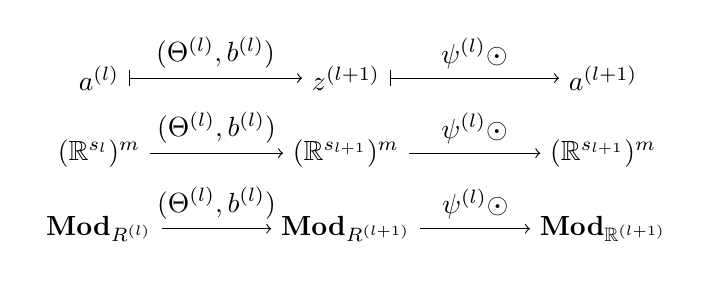
\begin{tikzpicture}
  \matrix (m) [matrix of math nodes, row sep=1.1em, column sep=4em, minimum width=1em]
  {
a^{(l)} & z^{(l+1)} & a^{(l+1)} \\ 
(\mathbb{R}^{s_l})^m & (\mathbb{R}^{s_{l+1}})^m & (\mathbb{R}^{s_{l+1}})^m  \\ 
\text{\textbf{Mod}}_{R^{(l)}} & \text{\textbf{Mod}}_{R^{(l+1)}} & \text{\textbf{Mod}}_{\mathbb{R}^{(l+1)}} \\ 
};
  \path[|->]
  (m-1-1) edge node [above] {$(\Theta^{(l)}, b^{(l)})$} (m-1-2)
  (m-1-2) edge node [above] {$\psi^{(l)} \odot$ } (m-1-3)
  ;
\path[->]
  (m-2-1) edge node [above] {$(\Theta^{(l)}, b^{(l)})$} (m-2-2)
  (m-2-2) edge node [above] {$\psi^{(l)} \odot$ } (m-2-3)
  ;
\path[->]
  (m-3-1) edge node [above] {$(\Theta^{(l)}, b^{(l)})$} (m-3-2)
  (m-3-2) edge node [above] {$\psi^{(l)} \odot$ } (m-3-3)
  ;
\end{tikzpicture}
\end{equation}

Since we need to operate with the activation function $\psi^{(l)} \odot$ elementwise, we (implicitly) equip $\text{\textbf{Mod}}_{R^{(l+1)}}$ with the Hadamard product.  In fact, with composition, we can represent the $l$th axon as 
\begin{equation}
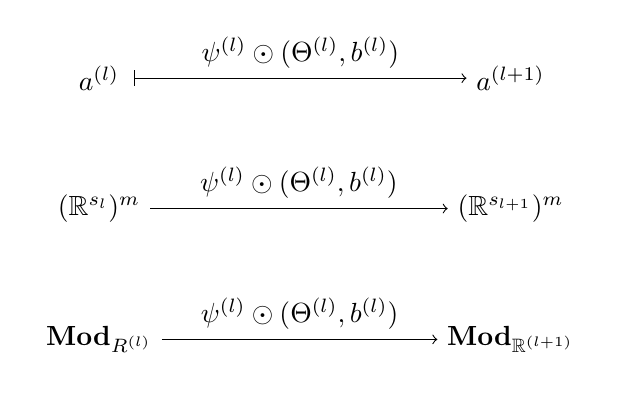
\begin{tikzpicture}
  \matrix (m) [matrix of math nodes, row sep=3.1em, column sep=10em, minimum width=2.5em]
  {
a^{(l)}  & a^{(l+1)} \\ 
(\mathbb{R}^{s_l})^m  & (\mathbb{R}^{s_{l+1}})^m  \\ 
\text{\textbf{Mod}}_{R^{(l)}}   & \text{\textbf{Mod}}_{\mathbb{R}^{(l+1)}} \\ 
};
  \path[|->]
  (m-1-1) edge node [above] {$\psi^{(l)} \odot (\Theta^{(l)}, b^{(l)})$} (m-1-2)
  ;
\path[->]
  (m-2-1) edge node [above] {$\psi^{(l)} \odot (\Theta^{(l)}, b^{(l)})$} (m-2-2)
  ;
\path[->]
  (m-3-1) edge node [above] {$\psi^{(l)} \odot (\Theta^{(l)}, b^{(l)})$} (m-3-2)
  ;
\end{tikzpicture} 
\end{equation}
The lesson is this: instead of thinking of layers, each separately, think of or focus on the relationship, the relations, between each layers, the axon, as one whole entity.  

Suppose we "feed in" input data $X$ into the first or $0$th layer of this NN.  This means that for $a^{(0)} \in \mathbb{R}^d$, 
\[
a^{(0)} = X^{(i)}
\]
for the $i$th (training) example.  

The "output" layer, layer $L$, should output the \emph{predicted} value, given $X$.  So 
\[
a^{(L)} \in \mathbb{R} \text{ or } \lbrace 0 ,1 , \dots K-1\rbrace \text{ or } [0,1]
\]
for regression, or classification (so it takes on discrete values) or the probability likelihood of being in some class $k$, respectively. 
 
The entire NN can mathematically expressed as follows: 
\begin{equation}
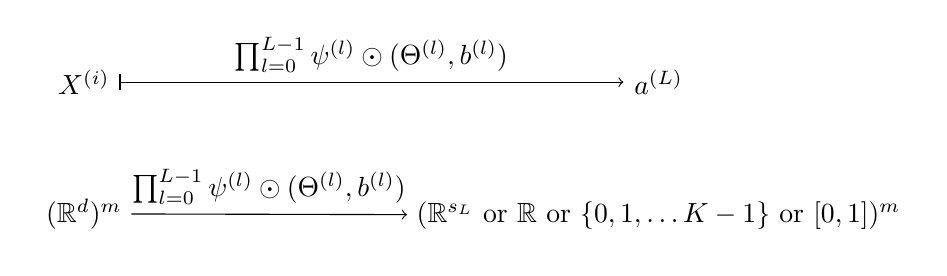
\begin{tikzpicture}
  \matrix (m) [matrix of math nodes, row sep=3.1em, column sep=10em, minimum width=2.5em]
  {
X^{(i)}  & a^{(L)} \\ 
(\mathbb{R}^{d})^m  & (\mathbb{R}^{s_L} \text{ or } \mathbb{R} \text{ or } \lbrace 0 ,1,\dots K-1\rbrace \text{ or } [0,1])^m  \\ 
};
  \path[|->]
  (m-1-1) edge node [above] {$\prod_{l=0}^{L-1} \psi^{(l)} \odot (\Theta^{(l)}, b^{(l)})$} (m-1-2)
  ;
\path[->]
  (m-2-1) edge node [above] {$\prod_{l=0}^{L-1} \psi^{(l)} \odot (\Theta^{(l)}, b^{(l)})$} (m-2-2)
  ;
\end{tikzpicture} 
\end{equation}


\part{Natural Language Processing (NLP) }

\url{https://github.com/davidadamojr/TextRank/blob/master/textrank/__init__.py}

\url{https://web.eecs.umich.edu/~mihalcea/papers/mihalcea.emnlp04.pdf}

\url{https://stackoverflow.com/questions/25315566/unicodedecodeerror-in-nltks-word-tokenize-despite-i-forced-the-encoding}

\section{TextRank}

\href{https://web.eecs.umich.edu/~mihalcea/papers/mihalcea.emnlp04.pdf}{TextRank: Bringing Order into Texts, Rada Mihalcea and Paul Tarau}

Mihalcea and Tarau \cite{MiTa}.  

Let $G=(V,E)$ be a directed graph with set of vertices $V$, set of edges $E$, $E\subset V \times V$.  

$\forall \, $ given vertex $V_i$, let $\text{In}(V_i) \subset V \equiv $ set of vertices that point to it $\equiv $ "predecessors", \\
let $\text{Out}(V_i) \subset V \equiv $ set of vertices that vertex $V_i$ points to "successors"

Let score $S:V \to \mathbb{R}$, 
\begin{equation}
 S(V_i) := (1-d) + d \sum_{j\in \text{In}(V_i) } \frac{1}{ (\text{Out}(V_j))} S(V_j)
\end{equation}
where $0\leq d\leq 1$.  

Usually $d=0.85$.  

Let $t\in \mathbb{Z}^+$.  Let $t=0$.  $\forall \, V_i \in V$, $S(V_i)(t=0) \in \mathbb{R}$, randomly assigned.  

Weighted graphs.  
\begin{equation}
WS(V_i) = (1-d) + d* \sum_{V_j \in \text{In}(V_i) } \frac{w_{ji} }{ \sum_{V_k \in \text{Out}(V_j) } w_{jk} } WS(V_j)
\end{equation}

$0\leq w_{ij} \leq 10$  

\subsection{Keyword Extraction}

2 vertices \emph{connected} if corresponding lexical units co-occur within window of max. $N$ words.  $2\leq N \leq 10$.  

\href{http://www.aclweb.org/anthology/I13-1062}{Topic Ranking}




\part{Notes}


Restricted Boltzmann machine - estimate a probability distribution

Recurrent neural network - creates an internal state of the network which allows it to exhibit dynamic temporal behavior


\href{http://stats.stackexchange.com/questions/181/how-to-choose-the-number-of-hidden-layers-and-nodes-in-a-feedforward-neural-netw}{How to choose the number of hidden layers and nodes in a feedforward neural network?}

``In sum, for most problems, one could probably get decent performance (even without a second optimization step) by setting the hidden layer configuration using just two rules: (i) number of hidden layers equals one; and (ii) the number of neurons in that layer is the mean of the neurons in the input and output layers.''


\url{https://www.quora.com/Natural-Language-Processing-What-are-algorithms-for-auto-summarize-text}

\url{https://arxiv.org/pdf/1602.03606.pdf}


\part{Unsupervised Learning}

\section{$k$-means clustering algorithm}

cf. \href{https://www.coursera.org/learn/machine-learning/lecture/93VPG/k-means-algorithm}{Coursera Machine Learning (Ng), Week 8, K-Means Algorithm}

$K$-means algorithm.  

Let $K\in \mathbb{Z}^+$.  \\
Let training set $\lbrace x_{(1)}, x_{(2)}, \dots x_{(m)} \in \mathbb{R}^d \rbrace$.  

Randomly initialize $K$ cluster centroids $\mu_1,\mu_2\dots \mu_k \in \mathbb{R}^d$.  

$\forall \, i = 1,2,\dots m$, 

Find $c^{(i)} \, \text{ (Ng's notation) } \equiv k_{(i)} $ s.t. 
\[
\min_{k=1,2,\dots K} \| x_{(i)} - \mu_k \|
\]
$\forall \, i = 1,2,\dots m$.  

$\forall \, k =1,2,\dots K$, 
\[
\mu_k := \frac{1}{ |C_k | } \sum_{ x_j \in C_k} x_j
\]
s.t. 
\[
\bigcup_{k=1}^K C_k = \lbrace x_{(1)}, x_{(2)}, \dots x_{(m)} \in \mathbb{R}^d \rbrace
\]

Only guaranteed to converge to local minimizers ($K$-means is NP-hard), polynomial time.  

Optimization objective:
\begin{equation}
J(c^{(1)}, \dots c^{(m)}, \mu_1 \dots \mu_k) \equiv J(k_{(1)}, \dots k_{(m)}, \mu_1 \dots \mu_k) = \frac{1}{m} \sum_{i=1}^m \| x_{(k)} - \mu_{ k_{(i)} } \| 
\end{equation}

So find 
\begin{equation}
\min_{ \substack{ c^{(1)} \dots c^{(m)} \\ \mu_1 \dots \mu_k } } J(c^{(1)}, \dots c^{(m)}, \mu_1 \dots \mu_k) \equiv \min_{ \substack{ k_{(1)} \dots   k_{(m)} \\ \mu_1 \dots \mu_k } } J( k_{(1)}, \dots k_{(m)}, \mu_1 \dots \mu_k) 
\end{equation}

\url{https://ocw.tudelft.nl/wp-content/uploads/Algoritmiek_Clustering.pdf}

\url{https://github.com/serban/kmeans/blob/master/cuda_kmeans.cu}

It is not possible for the cost function $J$ to sometimes increase (with number of iterations).  There must be a bug in the code.  cf. \href{https://www.coursera.org/learn/machine-learning/lecture/G6QWt/optimization-objective}{Optimization Objective}

1 important example or assumption to be made is the data points are independent of each other.  There exists no dependency between any data points.   

cf. \url{https://www.cse.buffalo.edu//faculty/miller/Courses/CSE633/Chandramohan-Fall-2012-CSE633.pdf}.  This also has references

\href{https://www.coursera.org/learn/machine-learning/lecture/drcBh/random-initialization}{Random Initialization}.  Randomly pick $K$ training examples from $\mathcal{X} \equiv \lbrace x_{(1)}, x_{(2)}, \dots x_{(m)} \in \mathbb{R}^d \rbrace$.  Then set $\mu_1\dots \mu_K$ to these $K$ examples.  

To avoid local minimization due to particular choice of $\mu_1, \dots \mu_k$, 

For $i=1, \dots $ number of times to randomize, $\lbrace$ 
Randomly initialize $K$-means \\
Run $K$-means.  Get $c^{(1)}, \dots c^{(m)} = k_{(1)} \dots k_{(m)}$, $\mu_1\dots \mu_K$  \\
Compute cost function (distortion) $J(c^{(1)}, \dots c^{(m)}, \mu_1 \dots \mu_K)\equiv J(k_{(1)}, \dots k_{(m)}, \mu_1 \dots \mu_K)$ \\
$\rbrace$

Then pick clustering that gave lowest cost $J(k_{(1)}, \dots k_{(m)}, \mu_1 \dots \mu_K)$

When $K=2-10$, random initialization of random initialization will have a huge advantage.  For $K>10$, not so much.  

\subsubsection{Choosing the value of $K$}
\href{https://www.coursera.org/learn/machine-learning/lecture/Ks0E9/choosing-the-number-of-clusters}{Choosing the Number of Clusters}

Plot $J$ vs. $K$ (number of clusters).  Find where change in $J$ with increase in $K$ changes itself.  

Suppose you run $K$-means using $K=3$ and $K=5$.  You find that the cost function $J$ is much higher for $K=5$ than for $K=3$.  What can you conclude? 

In the run with $K=5$, $K$-means got stuck in a bad local minimum.  You should try re-running $K$-means with multiple random initializations.  

International Conference on Computational Science, ICCS 2011.  Parallel $k$-Means Clustering for Quantitative Ecoregion Delineation Using Large Data Sets.  Jitendra Kumara, Richard T. Mills, Forrest M. Hoffman, William W. Hargrove.  
\url{http://citeseerx.ist.psu.edu/viewdoc/download?doi=10.1.1.431.3926&rep=rep1&type=pdf}

\subsubsection{Parallel $k/h$-means clustering}
From Stoffel and Belkoniene (1999) \cite{StBe1999}, 
Fig. 1 Pseudo code of the $k$-means and $h$-means algorithm:
\begin{lstlisting}
function K-MeanMainLoop {
	assign each object randomly to one cluster;
	do {
		for each object t in the database {
			nC = getNearestMean(t);
			insertIntoCluster(t,nC);
			recalculateMeans(t,nC);
		}
	} while at least one t changes its cluster
}
\end{lstlisting}
$k$-means.  

\begin{lstlisting}
function H-MeanMainLoop {
	assign each object randomly to one cluster;
	do {
		for each object t in the database {
			nC = getNearestMean(t);
			insertIntoCluster(t,nC);
		}
	recalculateMeans(t,nC);
	} while at least one t changes its cluster
}
\end{lstlisting}
$h$-means.  




\section{Dimensionality Reduction; Principal Component Analysis (PCA), Singular Value Decomposition (SVD)}  

\href{https://www.coursera.org/learn/machine-learning/lecture/0EJ6A/motivation-i-data-compression}{Motivation I: Data Compression}.  

Examples in $\mathbb{R}^2, \mathbb{R}^3$: projection.  


\subsection{Datapreprocessing; feature scaling, mean normalization}

\href{https://www.coursera.org/learn/machine-learning/lecture/ZYIPa/principal-component-analysis-algorithm}{Principal Component Analysis Algorithm}

Given a training set $\mathcal{X} = \lbrace x_{(1)}, x_{(2)}, \dots x_{(m)} \rbrace$, 

\subsubsection{Mean normalization}

\begin{equation}
\mu^j = \frac{1}{m} \sum_{i=1}^m x^j_{(i)}
\end{equation}
Then replace $\forall \, i =1\dots m , \, \forall \, j = 1\dots d$, $x^j_{(i)}$ with $x^j_{(i)} - \mu^j$

\subsubsection{Feature Scaling}


\subsection{Principal Component Analysis (PCA) algorithm}

\url{https://www5.in.tum.de/lehre/seminare/datamining/ss17/paper_pres/16_pca/paper.pdf}

Reduce data from $n$-dims. to $k$-dims.  

Compute "covariance matrix":

\begin{equation}
\Sigma := \frac{1}{m} \sum_{i=1}^m (X_{(i)})( X_{(i)})^T
\end{equation}

Compute "eigenvalues" of matrix $\Sigma$.  

2 arbitrary random variables $A,B$ with means $\mu_A,\mu_B$.  

\[
\text{cov}(A,B) = E[(A-\mu_A) (B-\mu_B)]  \qquad \, (1-dim.)
\]
$d$ dimensional case
\begin{equation}
\text{cov}(\mathbf{a},\mathbf{b}) = \frac{1}{m-1} \sum_{i=1}^m  (\mathbf{a}-\mathbf{\mu}_A) (\mathbf{b}- \mathbf{\mu}_B)^T = \frac{1}{m-1} \sum_{i=1}^m ( a - \mu_A)_i (b-\mu_B)_j = (\text{cov}(a,b))_{ij}
\end{equation}

Given data at vectors $\mathcal{X} = \lbrace \mathbf{x}_{(1)}, \mathbf{x}_{(2)}, \dots \mathbf{x}_{(m)} \in \mathbb{R}^d \rbrace$ with mean normalization \emph{done already }  $\mu  \equiv \mu_X = 0 $)

We want covariance 
\begin{equation}
	\text{cov}(\mathcal{X})_{jk} \equiv \Sigma_{\mathcal{X}} \equiv \Sigma = \frac{1}{m} \sum_{i=1}^m (X_{(i)} )_j (X_{(i)})_k 
\end{equation}
Given data as $R$-module
\begin{equation}
\begin{aligned}
	& X = X_{ i \mu} \qquad \, i = 1\dots m , \, \mu= 1\dots d \\ 
	& \text{cov}(X)_{\mu \nu } = \Sigma_X \equiv \Sigma = \frac{1}{m} X^T_{ \mu k } X_{k \nu}
\end{aligned}
\end{equation}

Suppose $Y:= XP$ for unitary (orthogonal) $P\equiv U$.  Now 
\[
X_{i\mu} P_{\mu \nu } = Y_{i\nu} , \qquad \, i = 1,\dots m , \, \nu = 1\dots k , \text{ where } d \equiv n \geq k
\]
Then
\begin{equation}
	\text{cov}(Y) = \frac{1}{m} Y^T Y = \frac{1}{m} P^T X^T XP = P^T \text{cov}{(X)} P
\end{equation}
$\forall \, $ real, symmetric (Hermitian) matrix $A\in \text{Mat}_{\mathbb{K}}(N,N)$, $A = U\Lambda U^T (=U\Lambda U^{\dag})$, $\Lambda = \text{diag}(\lambda_{11}, \dots \lambda_{NN} )$; also $U^T AU = \Lambda$.  

Clearly $(\Sigma_X)^T = \frac{1}{m} (X^TX)^T = \frac{1}{m} X^T X = \Sigma_X$.  So $\text{cov}(Y)$ is a \emph{diagonal matrix}.  

Then
\begin{equation}
\begin{gathered}
	(\Sigma_X P)_{\mu \nu } = ( \Sigma_X )_{\mu \rho } P_{\rho \nu} = (P \text{cov}(Y) )_{\mu \nu } = P_{\mu \rho} \lambda_{ \nu \nu} \delta_{\rho \nu } = \lambda_{ \nu \nu} P_{\mu \nu }
\end{gathered}
\end{equation}

The columns of $P$ are eigenvectors (that can be normalized) called \emph{principal components} $p_{\mu}$ of $X$, and construct 
\[
P = \left( \begin{matrix} p_1  & p_2  &  \dots & p_d \end{matrix} \right)
\]

cf. Holl (2016), \url{https://www5.in.tum.de/lehre/seminare/datamining/ss17/paper_pres/16_pca/paper.pdf}

\begin{theorem}
	Principal component $\mathbf{p}_i$ describes axis orthogonal to $p_1 \dots p_{i-1}$ along which original data set has largest variance.  
\end{theorem}

\begin{proof}
	Along axis $v\in \mathbb{R}^d$, project $X$ onto $v$.  $Xv = X_{i\nu } v_{\nu}$, \, $i=1\dots m$, $\nu = 1\dots d$.  

\[
\begin{gathered}
\text{var}(Xv) = \frac{1}{m-1} (Xv)^T Xv = \frac{1}{m} (Xv)^T_{ \  \  i} (Xv)_i = \frac{1}{m} (v^T X^T)_i X_{i\nu} v_{\nu} = \frac{1}{m} ( v_{\mu} X_{i \mu} ) X_{i\nu } v_{\nu} = v_{\mu} \Sigma_{\mu \nu } v_{\nu}
\end{gathered}
\]	
Normalize the variance
\begin{equation}
	\text{var}(Xv) \equiv \text{var}_v(X) = \frac{ v_{\mu} \Sigma_{\mu \nu }v_{\nu } }{ v_{\mu} v_{\mu} } = \frac{ v^T \Sigma v}{ v^T v} 
\end{equation}
 
Maximize $\text{var}_v(X)$.  

Goal, under given orthogonality constraints, i.e. 
\[
v = \text{argmax}_{ \substack{ v\neq 0 \\ v\perp U_{i-1} } } \frac{ v^T \text{cov}(X) v}{ v^T v} 
\]
where $U_{i-1}$ is subspace of $\mathbb{R}^d$, spanned by $p_1$ through $p_{i-1}$, called Rayleigh quotient of $\text{cov}(X)$ and $v$.  

Recall \emph{Courant-Fischer minimax thm., Courant-Fischer thm.}: 

\begin{theorem}[Courant-Fischer (minimax) thm.]
Given $A\in \text{Mat}_{\mathbb{K}}(n,n)$, $A$ Hermitian.  

Let $\lbrace S_k^{\alpha} \rbrace_{\alpha \in I_k} \equiv $ set of all $k$-dim. linear subspaces of $\mathbb{C}^n$, , eigenvalues of $A$, $\lambda_1 \leq \dots \leq \lambda_n$.  

Then 
\begin{equation}
\begin{aligned}
	& \min_{\alpha \in I_k} \max_{ x\in S_k^{\alpha} \backslash \lbrace 0 \rbrace } \frac{ \langle Ax,x \rangle }{  \| x\|^2  } = \lambda_k \\ 	
	& \max_{\alpha \in I_{n-k+1} } \min_{x  \in S^{\alpha}_{n-k+1}  \backslash \lbrace 0 \rbrace  } \frac{ \langle Ax,x \rangle }{ \| x \|^2 } = \lambda_k
\end{aligned}
\end{equation}
\end{theorem} 

With Courant-Fischer minimax thm., 
\begin{equation}\label{Eq:PCA01maxvar}
\max_{ \substack{ v\neq 0 \\ v\perp U_{i-1} } } \frac{ v^T \text{cov}(X) v}{ v^T v} = \lambda_i 
\end{equation}
Now, it remains to prove that eigenvector corresponding to $\lambda_i$, fulfills Eq. \ref{Eq:PCA01maxvar}.  

Recall eigenvalue eqn. 
\[
\begin{gathered}
	\Sigma p = \lambda_i p \text{ i.e. } \Sigma_{\mu \rho } p_{\rho \nu} = \lambda_{ \nu \nu} p_{\mu \nu } \\ 
 \frac{ p_{\nu}^T \text{cov}(X) p_{\nu } }{ p_{\nu}^T p_{\nu} } = \frac{ p_{\nu}^T \Sigma p_{\nu} }{ p_{\nu}^T p_{\nu} } = \frac{ \lambda_{\nu}  p_{\nu}^T p_{\nu} }{ p_{\nu}^T p_{\nu} } = \lambda_{\nu}
\end{gathered}
\]
$\Longrightarrow$ so eigenvectors $\mathbf{p}_{\nu}$ (principal component) maintain maximal variance.  


\end{proof}

PCA also allows us to eliminate dims. from dataset while minimizing error incurred, i.e. losing least amount of data.  

\begin{theorem}\label{Thm:PCAminerr}
PCA minimize total squared error experienced by eliminating all but $\widehat{n}$ of the $n$-dims.  
\end{theorem}

\begin{proof}
Represent $\forall \, $ data pt. $x_{(i)} \in \mathbb{K}^n$ as linear combination of orthonormal basis $\mathbf{b}_1 , \dots \mathbf{b}_n$  
\[
\mathbf{x}_{(i)} = \sum_{j=1}^n \alpha_{ij} \mathbf{b}_j
\]

Consider $\widehat{x}_{(i)} = \sum_{j=1}^{\widehat{n}} \alpha_{ij}\mathbf{b}_j , \quad \, \widehat{n} \leq n $

\begin{equation}
\text{err}_{\widehat{n}} = \sum_{i=1}^m \|  \mathbf{x}_{(i)} - \widehat{x}_{(i)} \|^2 = \sum_{i=1}^m \| \sum_{j=\widehat{n}+1}^n \alpha_{ij} \mathbf{b}_j \|^2 = \sum_{i=1}^m \sum_{ j = \widehat{n}+1}^n \| \alpha_{ij} \|^2 
\end{equation}
Since $\mathbf{b}_j$ orthonormal, $\mathbf{b}_j^T \mathbf{b}_j = \sum_{\mu = 1}^n (b_j)_{\mu}(b_j)^{\mu} = 1$, or 
\[
\begin{gathered}
\mathbf{b}_j^T \mathbf{b}_k =\sum_{\mu = 1}^n (b_j)_{\mu} (b_k)^{\mu} = \delta_{jk} \\
	\alpha_{ij} = \langle \mathbf{x}_{(i)} , \mathbf{b}_j \rangle = \mathbf{b}_j^T \mathbf{x}_{(i)} = (\mathbf{x}_{(i)}^T ) \mathbf{b}_j = x_{(i)}^{\mu} (b_j)_{\mu} 
\end{gathered}
\]

Then
\[
\begin{gathered}
\sum_{i=1}^m \sum_{j= \widehat{n}+1}^n \| \alpha_{ij} \|^2 = \sum_{i=1}^m \sum_{j =\widehat{n}+1}^n x^{\mu}_{(i)} (b_j)_{\mu} x^{\nu}_{(i)} (b_j)_{\nu} = \sum_{j=\widehat{n}+1}^n (b_j)_{\mu} \sum_{i=1}^m x^{\mu}_{(i)} x^{\nu}_{(i)} (b_j)_{\nu} = m\sum_{j=\widehat{n}+1}^n (b_j)_{\mu} \Sigma_{\mu \nu} (b_j)_{\nu} = \\
= m \sum_{j=\widehat{n}+1}^n \frac{b_j^T \Sigma b_j}{ b_j^T b_j }
\end{gathered}
\]
If $\widehat{n} = n-1$, then error minimized by $b_n = p_n $ (Courant-Fishcer Thm.).  

Because $b_j$ orthogonality by def., conclude that $b_j=p_j$ minimized $\text{err}_{\widehat{n}}  \quad \, \forall \, \widehat{n}$  
\end{proof}


Applications of PCA are exploratory data analysis, through dimensional reduction, dimensional reduction itself, and regression problems, since by Thm. 2, \ref{Thm:PCAminerr}, then using PCA minimizes the error incurred by the regression. Holl (2016), \url{https://www5.in.tum.de/lehre/seminare/datamining/ss17/paper_pres/16_pca/paper.pdf}




\href{https://www.coursera.org/learn/machine-learning/lecture/X8JoQ/reconstruction-from-compressed-representation}{Reconstruction from Compressed Representation}  

Suppose we run PCA with $k=n$, so that the dimension of the data is not reduced at all.  (This is not useful in practice but is a good thought exercise.)  Recall that the percent/fraction of variance retained is given by: $\frac{ \sum_{i=1}^k S_{ii} }{ \sum_{i=1}^n S_{ii} }$.  Which of the following will be true?  

$U_{\text{reduce}} $ will be an $n\times n$ matrix.  $x_{\text{approx}} = x$ for every example $x$.  The percentage of variance retained will be 100 \%.  

To choose $k$ (number of principal components), do Singular Value Decomposition (SVD).  With $S$, the diagonal matrix, and its diagonal entries, $s_{\nu \nu}$, $\nu = 1\dots n\equiv d$, then, for given $k$, 
\[
\begin{gathered}
	\frac{ \frac{1}{m} \sum_{i=1}^m \| \mathbf{x}_{(i)} - \mathbf{x}_{\text{approx}, (i)} \|^2 }{ \frac{1}{m} \sum_{i=1}^m \| \mathbf{x}_{(i)} \|^2 } = 1- \frac{ \sum_{\nu =1}^{ \widehat{n} }  \frac{ \langle p_{\nu} , \Sigma p_{\nu}  \rangle }{ \langle p_{\nu} , p_{\nu} \rangle } }{ \sum_{\nu=1}^n \frac{ \langle p_{\nu} , \Sigma p_{\nu} \rangle }{ \langle p_{\nu}, p_{\nu} \rangle } } = 1 - \frac{ \sum_{\nu=1}^{\widehat{n} } s_{\nu \nu } }{ \sum_{i=1}^n s_{\nu \nu } }
\end{gathered}
\]

\subsubsection{Supervised learning speedup}  cf. \href{https://www.coursera.org/learn/machine-learning/lecture/RBqQl/advice-for-applying-pca}{Advice for Applying PCA}.   Run PCA only on training set.  


\textbf{Bad use of PCA: To prevent overfitting}.  

It's not what PCA does.  Use regularization instead to address overfitting.  

\textbf{PCA is sometimes used where it shouldn't be}.  (e.g. Design of ML system).  

How about doing the whole thing without using PCA?

Before implementing PCA, first try running whatever you want to do with the original/raw data $x_{(i)}$.  Only if that doesn't dow hat you want, then implement PCA and consider using $z_{(i)}$.  



Ng uses PCA to speed up learning algorithms alot..  

Also, remember compress data, reduce memory data requirements.  

\section{PageRank}  

cf. Gleich (2015) \cite{Glei2015}

Let $i=1,2\dots N$; $N=$ total number of "states".  If "states" are represented as vertices $v_i \in V \in \mathbf{\text{(Finite)Set}}$, then $i$ are some choice of labels for $v_i$'s.  

Let $P_{ij} :=$ probability of transitioning from $j$ to $i$.  

Clearly $P(i) \equiv $ probability of state $i$ in next iteration $=P_{ij}P(j)$.  

Let $\mathbf{v}:\lbrace 1,2, \dots N \rbrace \to \mathbb{R}$, $0\leq \mathbf{v}(i) \leq 1$.  

$\mathbf{v}(i) = $ (normalized) "probability" (likelihood) $i \in \lbrace 1,2, \dots N \rbrace$ of \emph{teleportation distribution} of randomly transitioning or teleporting for state $i$.  

Note that this $\mathbf{v}$ is also represented as vector:
\[
\mathbf{v} \xrightarrow{ \text{ vectorize } } \mathbf{v} \in \mathbb{R}^N
\]
$\alpha \in \mathbb{R}^+$, $0\leq \alpha \leq 1$ is a tuned parameter.  

Then Gleich considers this as the (vectorized) PageRank algorithm:
\begin{equation}
\alpha P_{ij}x_j + (1-\alpha) v_i =0 
\end{equation}
with $\mathbf{x}$ being what Gleich denotes as the PageRank vector.  

So in Gleich's notation, 
\begin{equation}
(\alpha \mathbf{P} + (1-\alpha)\mathbf{v} \mathbf{e}^T )\mathbf{x} = \mathbf{x}  \text{ or } ( \mathbf{1} - \alpha \mathbf{P}) \mathbf{x} = (1-\alpha) \mathbf{v}
\end{equation}
cf. Eq. (2.1) and (2.2) of Gleich (2015) \cite{Glei2015}, respectively.  

Following Page, Brin, Motwani, and Winograd (1998) \cite{PBMW1998}, and their notation now:

let $u$ be a webpage.  $u \equiv x \in X$, where $X$ is a set (that could represent the set of vertices $X$).  Let $Y = $ set of all edges of this graph.  

Let $F_u := $ set of pages that $u$ points to, i.e. 
\begin{equation}
F_u = \lbrace x | x\in X, \begin{aligned} & u = o(y) \\
& x = t(y) \end{aligned} \text{ for some } y \in Y \rbrace 
\end{equation}

Let $B_u : = $ set of pages that point to $u$, i.e. 
\begin{equation}
	B_u = \lbrace x | x\in X, \begin{aligned} & x = o(y) \\
	& u= t(y) \end{aligned} \text{ for some } y\in Y \rbrace 
\end{equation}
$N_u = |F_u| = $ number of links from $u$.  Let $c\in \mathbb{R}$ normalization factor (so total rank of all webpages constant).  

Define simple ranking $R$, 
\begin{equation}
\begin{aligned}
& R:X \to \mathbb{R}  \\
& R(u) = c\sum_{ v\in B_u } \frac{R(v) }{N_v}
\end{aligned}
\end{equation}

Consider 
\[
\begin{gathered}
\sum_{u \in X} R(u) = c\sum_{u \in X} \sum_{v\in B_u} \frac{R(v) }{ N_v} \Longrightarrow \frac{ \sum_{u\in X} R(u)}{ \sum_{u\in X} \sum_{ v\in B_u } \frac{R(v)}{N_v} } = c   \\
	c=\frac{R(u)}{ \sum_{v\in B_u } \frac{R(v) }{ N_v} }
\end{gathered}
\]

Consider $u \in X$.  $\forall \, v \in B_u$, $N_v \geq 1$ (since connected graph \textbf{must} be connected, by definition).  

$c<1$ since there's the case of $F_u = \emptyset$ and "their weight is lost from system (cf. Sec. 2.7 of Page, Brin, Motwani, and Winograd (1998) \cite{PBMW1998})".  

There's a problem if we have the case of circuits of size $n=1$, $n=2$.  To overcome existence of circuits (rank sinks), 
\begin{definition}
	Let $E(u) := $ source of ranks.  
	
	$R' \equiv $ PageRank, 
	\begin{equation}
	\begin{aligned}
	& R' : X\to \mathbb{R}  \\
	& R'(u) = c\sum_{v\in B_u } \frac{R'(v)}{N_v} + cE(u)
	\end{aligned}
	\end{equation}
s.t. $c$ maximized, $\| R' \|_1 = 1$ ( $\| R' \|_1$ denotes the $L_1$ norm of $R'$)	
\end{definition}

Generalizing this, for $A_{uv} \equiv $ "likelihood of transition \textbf{from} $v$ \textbf{to } $u$, so that $A_{uv} = \frac{1}{N_v}$ for this special case.  

\[
R'(u) = c\sum_{v\in B_u } A_{uv} R'(v) + cE(u)
\]
Both Page, Brin, Motwani, and Winograd and Gleich rewrites this as 
\[
R' = c(A + E\mathbf{e}^T)R'
\]
with $\mathbf{e}$ being a column of $1$'s.  

Indeed, 
\[
E_{i1} (\mathbf{e}^T)_{1k} R'_{k1} = E_{i1} \| R' \|_1 = E_{i1} 
\]
since $\| R' \|_1=1$ by (defined) normalization.  

$E$ is a user-defined parameter, possibly uniform $\forall \, u \in X$.  
\begin{equation}
R'(u) - c\sum_{v\in B_u} A_{uv} R'(v) = cE(u)
\end{equation}

\subsubsection{PageRank algorithm by Page, Brin, Motwani, and Winograd (1998) \cite{PBMW1998}}
	
cf. 12.6 \emph{Computing Page Rank}, pp. 6 of Page, Brin, Motwani, and Winograd (1998) \cite{PBMW1998}.  

Let $S$ be almost any vector over $X$; $\begin{aligned} & \quad \\
	& S:X \to \mathbb{R} \\
	& S(u) \geq 0 \end{aligned}$, \, (e.g. $E$).  Then, for iterations $t= 0,1,\dots \in \mathbb{Z}^+$, 
and so for 
\[
R: X \times \mathbb{Z}^+ \to \mathbb{R}
\]
Then 
\[
\begin{gathered}
R(u,0) \equiv R_0(u) = S(u)  \qquad \, (R_0 \leftarrow  S)
\end{gathered}
\]

$ \forall \, t \in \mathbb{Z}^+, \,$ 
\[
\begin{gathered}
	 \forall \, u \in X, \, R(u,t+1) = A_{uv} R(v,t)  \\
	d= ( \| R(u,t) \|_1 - \| R(u,t+1) \|_1 ) \\
	R(u,t+1) = R(u,t+1)+dE \\
	\delta = \| R(u,t+1) - R(u,t) \|_1 
\end{gathered}
\]
while $\delta > \epsilon$.  

Compare this to the iteration by Gleich (2015) \cite{Glei2015}: 
\begin{equation}
\mathbf{x}^{(k+1)} = \alpha \mathbf{P} \mathbf{x}^{(k)} + (1-\alpha) \mathbf{v} 
\end{equation}
where
\[
\mathbf{x}^{(0)} = \mathbf{v} \text{ or } \mathbf{x}^{(0)} = 0
\]

Indeed, 
\begin{equation}
\begin{gathered}
R(u) - R(u;t+1) = (\alpha A_{uv} R(v) + (1-\alpha) E) - ( \alpha A_{uv} R(v,t) + (1-\alpha ) E) = \alpha A_{uv}(R(v) - R(v,t) )
\end{gathered}
\end{equation}
Indeed, $R(u,t)$ converges to $R(u)$.  

\subsubsection{PageRank Vector Iteration Implementation \cite{TUMHPC2016}}

cf. Nov. 14. Dwarf No. 2 - Sparse Linear Algebra lecture by Dr. Bader \cite{TUMHPC2016}, \url{http://www5.in.tum.de/lehre/vorlesungen/hpc/WS16/sparseLA.pdf}  

Define 
\begin{equation}
	A_{ij} \in \text{Mat}_{\mathbb{R}}(N,N) 
\end{equation}
where $N=$ total number of webpages (vertices) $= |X|$, with $A_{ij}$ defined as 
\begin{equation} 
A_{ij} = \begin{cases} 
1 & \text{ if $ \exists \, $ edge $ y \in Y$ \textbf{ from } $j$ \textbf{ to } $i$ (i.e. $\exists \, y \in Y$ s.t. $\begin{aligned} & \quad \\ & o(y) = x_j \\ & t(y) = x_i \end{aligned}$ } ) \\
0 & \text{ otherwise } \end{cases}   
\end{equation}
with 
\begin{equation}
N_j = \sum_{i=1}^N A_{ij} = \text{ total number of links from $j$th webpage (vertex) } = |F_j |
\end{equation}
and so \emph{define} $B_{ij}$
\begin{equation}
\begin{aligned}
	& B_{ij} \in \text{Mat}_{\mathbb{R}}(N,N) \\ 
	& B_{ij} := \frac{1}{N_j} A_{ij}
\end{aligned}
\end{equation}

Compute PageRank vector via vector iteration 
\begin{equation}
\begin{gathered} 
\mathbf{x}^{(m)} = \alpha B \mathbf{x}^{(m-1)} + (1-\alpha) \frac{1}{N} \mathbf{e} \text{i.e. }  \\
R(u;t+1) = \alpha B_{uv} R(v;t) + (1-\alpha ) E(u)
\end{gathered}
\end{equation}

$B$ is a sparse matrix, so use SpMV, i.e. sparse matrix vector multiplication.  

Now, we should talk about \emph{Sparse Linear Algebra}.  

\section{Data Structures for Sparse Matrices}  

cf. Part II: Data Structures for Sparse Matrices in Nov. 14. Dwarf No. 2 - Sparse Linear Algebra lecture by Dr. Bader \cite{TUMHPC2016}, \url{http://www5.in.tum.de/lehre/vorlesungen/hpc/WS16/sparseLA.pdf}.  

\subsection{Coordinate Scheme (aka Triple Scheme) }

We want
\begin{equation}
\begin{gathered}
A_{ij} \in \text{Mat}_{\mathbb{F}}(N_i,N_j) \mapsto (a_{ij},i,j)\mathbb{F}  \times \mathbb{Z}^+ \times \mathbb{Z}^+
\end{gathered}
\end{equation}
Let $K \in \mathbb{Z}^+ = $ total number of \textbf{nonzero} entries in $A_{ij}$.  

The coordinate scheme is implemented either as an array of struct (of size $K$), i.e. 
\begin{equation}
\begin{aligned}
& M:\mathbb{Z}^+ \to \mathbb{F} \times \mathbb{Z}^+ \times \mathbb{Z}^+ \\
& M(I) = (A(I), i(I), j(I) )
\end{aligned}
\end{equation}
or struct of array, i.e. 
\begin{equation}
	\begin{gathered}
	A_{ij} \in \text{Mat}_{\mathbb{F}}(N_i,N_j) \mapsto M \in (\mathbb{Z}^+ \to \mathbb{F}) \times ( \mathbb{Z^+} \times \mathbb{Z}^+)^2 \text{ with } \\
	M_1(I) = A(I) , M_2(I) = i(I), M_3(I) = j(I)
	\end{gathered}
\end{equation}
used, e.g. in Matlab, or as input format (format to input in ).  Note also that it's possibly not sorted, i.e. $i=i(I), j= j(I)$ may not follow any lexicographic order, depending on $I$.  

\subsection{Compressed Row Storage (CRS)  }

2 arrays of size $K$ with $a_{ij}$ and $j$, i.e. consider $a: \lbrace 1, 2 , \dots K \rbrace \to \mathbb{F}$.  

\begin{equation}
\begin{gathered}
A_{ij} \in \text{Mat}_{\mathbb{F}}(N_i , N_j) \mapsto \begin{aligned} 
	& a:\lbrace 1,2, \dots K \rbrace \to \mathbb{F}, \, \\ 
	& j : \lbrace 1,2, \dots K \rbrace \to \mathbb{Z}^+ , \, \\
	& IA: \lbrace 0 ,1,\dots N_i \rbrace \to \mathbb{Z}^+ \in \text{Hom}(\mathbb{Z}^+,\mathbb{F}), \text{Hom}(\mathbb{Z}^+,\mathbb{Z}^+)^2
\end{aligned}
\end{gathered}
\end{equation}

Note that we are using left-to-right, top-to-bottom "row-major" order, which is amenable to so-called (thread) warp coalescing for memory usage/optimization in CUDA C/C++.  

So, to reiterate, we have \\
$a(k) = a_{ij}$ for some surjective $(i,j) ]\mapsto k$ \\
$j(k) \in \mathbb{Z}^+$ 
\[
IA(i) = \begin{cases}0  & \text{ if } i = 0 \\
& IA(i-1) + (\text{number of nonzero elements of $(i-1)$th row in original matrix}) \end{cases}
\]
Let's take a look at $IA: \lbrace 0,1,\dots N_i \rbrace \to \mathbb{Z}^+$ in greater detail.  Consider these simple cases:  \\
$IA(0)= 0$ \\
$IA(i) = IA(i-1) + (\text{number of nonzero elements of $(i-1)$th row in original matrix, with $i=0,1,\dots N_i-1$, in this particular case)}$

And so 
\[
IA(1) = 0+\text{number of nonzero elements of $0$th row in original matrix}
\]
(we started counting from $0$ in this case, \textbf{not} from $1$).  

\[
IA(2) = IA(1)+\text{number of nonzero elements of "$1$th" row in original matrix}
\]
(or "second" row, counting from, starting from $1$) 

Clearly $IA(N_i)=K$ since 
\[
IA(i) = \sum_{l=0}^{i-1} (\text{number of nonzero elements in $l$th row ($0$-based country; $l=0,1,\dots N_i-1$)})
\]
For $1$-based counting (i.e. row $=1,2,\dots N_i$), 
\begin{equation}
IA(i) = \begin{cases} 0 & \text{ if } i=0 \\
 \sum_{l=1}^i (\text{number of nonzero elements in $l$th row}) & \end{cases}
\end{equation}
and so for 
\[
(i,j ) \in \lbrace 1,2, \dots N_i \rbrace \times \lbrace 1,2, \dots N_j \rbrace \mapsto IA(i-1) + j = k \in \lbrace 1,2, \dots K \rbrace 
\]
\[
A_{ij}x_j = a(IA(i-1+j))x_j(j(k))
\]

\subsection{ELLPACK Format}

$\forall \, i \in \lbrace 1, 2, \dots N_i \rbrace$, let number of nonzero elements in $i$th row $\leq K_{\text{max}}$.  

Then consider storing values in $a_{ik} \in \text{Mat}_{\mathbb{F}}(N_i,K_{\text{max}})$.  

Store column indices $j\in \lbrace 1,2, \dots N_j \rbrace$ (notice "$1$-based counting") in $j\in \text{Mat}_{\mathbb{F}}(N_i,K_{\text{max}})$.  

$j_{ik} =0$ if there is $0$ entry for $A_{ij}=0$.  




\end{multicols*}
\begin{thebibliography}{9}
\bibitem{HTF2009}
Trevor Hastie, Robert Tibshirani, Jerome Friedman.   \textbf{The Elements of Statistical Learning: Data Mining, Inference, and Prediction}, Second Edition (Springer Series in Statistics) 2nd ed. 2009. Corr. 7th printing 2013 Edition.  ISBN-13: 978-0387848570.  \url{https://web.stanford.edu/~hastie/local.ftp/Springer/OLD/ESLII_print4.pdf}

\bibitem{CS2013}
Jared Culbertson, Kirk Sturtz.  \emph{Bayesian machine learning via category theory}.  \href{http://arxiv.org/abs/1312.1445}{arXiv:1312.1445} [math.CT]

\bibitem{CS344}
John Owens.  David Luebki.  \emph{Intro to Parallel Programming}.  \emph{CS344}.  \textbf{\href{https://www.udacity.com/}{Udacity}}  
  
\url{http://arxiv.org/abs/1312.1445} Also, \url{https://github.com/udacity/cs344}  

\bibitem{CS229}
CS229 Stanford University.  \url{http://cs229.stanford.edu/materials.html}


\bibitem{Fitz}
Richard Fitzpatrick.  ``Computational Physics.''  \url{http://farside.ph.utexas.edu/teaching/329/329.pdf}

\bibitem{LISA2015}
LISA lab, University of Montreal.  Deep Learning Tutorial.  \url{http://deeplearning.net/tutorial/deeplearning.pdf}  September 2015.  



\bibitem{Horn1991}
Kurt Hornik. ``Approximation Capabilities of Muitilayer Feedforward Networks.''  \textbf{Neural Networks}, Vol. 4, pp. 251-257. 1991

\bibitem{HSW1989}
Kurt Hornik. Maxwell Stinchcombe and Halbert White.  ``Multilayer Feedforward Networks are Universal Approximators.''  \textbf{Neural Networks}, Vol. 2, pp. 359-366, 1989.  


\bibitem{JZS2015}
Rafal Jozefowicz, Wojciech Zaremba, Ilya Sutskever.  "An Empirical Exploration of Recurrent Network Architectures."  \emph{Proceedings of the 32 nd International Conference on Machine Learning}, Lille, France, 2015. JMLR: W\&CP volume 37.

\bibitem{GBC2016}
Ian Goodfellow, Yoshua Bengio, and Aaron Courville.  \textbf{Deep Learning} (Adaptive Computation and Machine Learning series).  The MIT Press (November 18, 2016).  




\bibitem{Nowa2008}
Thomas Nowak.  ``Implementation and Evaluation of a Support Vector Machine on an 8-bit Microcontroller.''  Univ.Ass. Dipl.-Ing. Dr.techn. Wilfried Elmenreich Institut f\"{u}r Technische Informatik Fakult\"{a}t f\"{u}r Informatik Technische Universit\"{a}t Wien.  Juli 2008.  \url{https://www.lri.fr/~nowak/misc/bakk.pdf}



\bibitem{STCr2000}
J.  Shawe-Taylor  and  N.  Cristianini,  Support  Vector  Machines  and  other  kernel-based  learning  methods,
Cambridge University Press (2000).



\bibitem{ChZa2013}
Edwin K. P. Chong and Stanislaw H. Zak.  \textbf{An Introduction to Optimization}.  4th Edition.  Wiley.  (January 14, 2013).  ISBN-13: 978-1118279014
  
\bibitem{Nara2015}
Lecture by Harikrishna Narasimhan.  \emph{Optimization Tutorial 3: Projected Gradient Descent, Duality}.  \textbf{E0 270 Machine Learning}.  Jan 23, 2015.  \url{http://drona.csa.iisc.ernet.in/~e0270/Jan-2015/Tutorials/lecture-notes-3.pdf}

\bibitem{Bish2007}
Christopher M. Bishop.  \textbf{Pattern Recognition and Machine Learning} (Information Science and Statistics).  Springer (October 1, 2007).  ISBN-13: 978-0387310732


\bibitem{CFZ2009}
Bertrand Clarke, Ernest Fokoue, Hao Helen Zhang.   \textbf{Principles and Theory for Data Mining and Machine Learning} (Springer Series in Statistics)  Springer; 2009 edition (July 30, 2009).  ISBN-13: 978-0387981345
 

\bibitem{Ngu2007}
Hubert Nguyen. \textbf{GPU Gems 3}.  Addison-Wesley Professional (August 12, 2007).  ISBN-13: 978-0321515261.  Also made available in its entirety online at \url{https://developer.nvidia.com/gpugems/GPUGems3/gpugems3_pref01.html}

\bibitem{Pedr2011}
  Scikit-learn: Machine Learning in Python, Pedregosa \emph{et al.}, \textbf{JMLR 12}, pp. 2825-2830, 2011.


\bibitem{CySi2009}
Bogus\l{} aw Cyganek.  J. Paul Siebert.  \textbf{An Introduction to 3D Computer Vision Techniques and Algorithms}.  Wiley.  2009.  ISBN 978-0-470-01704-3

 \bibitem{HaZi2003}
Richard Hartley.  Andrew Zisserman.  \textbf{Multiple View Geometry in Computer Vision}  Second Edition.  \emph{Cambridge University Press.}  2003.  ISBN-13 978-0-511-18618-9 eBook (EBL)

\bibitem{JLee2012}
John Lee, \textbf{Introduction to Smooth Manifolds} (Graduate Texts in Mathematics, Vol. 218), 2nd edition, Springer,  2012, ISBN-13: 978-1441999818

\bibitem{JLee2009}
Jeffrey M. Lee. \textbf{Manifolds and Differential Geometry}, \emph{Graduate Studies in Mathematics} Volume: 107, American Mathematical Society, 2009. ISBN-13: 978-0-8218-4815-9



\bibitem{ChLi2011}
  C.-C. Chang and C.-J. Lin. \emph{LIBSVM : a library for support vector machines}. \textbf{ACM Transactions on Intelligent Systems and Technology}, 2:27:1--27:27, 2011. 

\bibitem{Pla1998}
  J. Platt. \emph{Fast training of support vector machines using sequential minimal optimization}. In A. Smola B. Schölkopf, C. Burges, editor, \textbf{Advances in Kernel Methods: Support Vector Learning}. MIT Press, Cambridge, MA, 1998.

\bibitem{HCL}
Chih-Wei Hsu, Chih-Chung Chang, and Chih-Jen Lin.  \emph{A Practical Guide to Support Vector Classification}.  \url{http://www.ee.columbia.edu/~sfchang/course/spr/papers/svm-practical-guide.pdf}

\bibitem{MiTa}
Rada Mihalcea and Paul Tarau.  "TextRank: Bringing Order into Texts."  
\url{https://web.eecs.umich.edu/~mihalcea/papers/mihalcea.emnlp04.pdf}  

\bibitem{Glei2015}
David F. Gleich.  \emph{PageRank Beyond the Web.}  \textbf{SIAM Review}.  Vol. 57, No. 3, pp. 321-363 2015  
  
\bibitem{PBMW1998}  
Page, Lawrence and Brin, Sergey and Motwani, Rajeev and Winograd, Terry.  "The PageRank Citation Ranking: Bringing Order to the Web." Technical Report. Stanford InfoLab.  1998.  \url{http://ilpubs.stanford.edu:8090/422/1/1999-66.pdf}  
  
\bibitem{TUMHPC2016}
Prof. Dr. Michael Bader, with Alexander P\"{o}ppl, Valeriy Khakhutskyy (Tutorials).  High Performance Computing (HPC) - Algorithms and Applications - Winter 16/17.  Informatics V - Scientific Computing.  Technical University of Munich (TUM)
\url{https://www5.in.tum.de/wiki/index.php/HPC_-_Algorithms_and_Applications_-_Winter_16}


\bibitem{AnNg}
Andrew Ng.  \href{https://www.coursera.org/learn/machine-learning/home/welcome}{Machine Learning}.  \href{https://www.coursera.org}{coursera}


\bibitem{StBe1999}
Kilian Stoffel and Abdelkader Belkoniene.  \emph{Parallel $k/h$-Means Clustering for Large Data Sets}.  Euro-Par'99, LNCS 1685, pp. 1451-1454, 1999.  Springer-Verlag Berlin Heidelberg 1999

\url{https://grid.cs.gsu.edu/~wkim/index_files/papers/parkh.pdf}

\bibitem{theano}
Theano Development Team. \href{http://arxiv.org/pdf/1605.02688.pdf}{“Theano: A Python framework for fast computation of mathematical expressions”}. 

\bibitem{JRotman2010}
Joseph J. Rotman, \textbf{Advanced Modern Algebra} (Graduate Studies in Mathematics) 2nd Edition, American Mathematical Society; 2 edition (August 10, 2010), ISBN-13: 978-0821847411

\bibitem{JLee2009}
Jeffrey M. Lee. \textbf{Manifolds and Differential Geometry}, \emph{Graduate Studies in Mathematics} Volume: 107, American Mathematical Society, 2009. ISBN-13: 978-0-8218-4815-9

\bibitem{Conl2008}
Lawrence Conlon.  \textbf{Differentiable Manifolds} (Modern Birkhäuser Classics).  2nd Edition.  Birkhäuser; 2nd edition (October 10, 2008).  ISBN-13: 978-0817647667

\bibitem{SageMath2017}
The Sage Development Team.  Sage Reference Manual: Category Framework.  Release 7.6.  Mar. 25, 2017.  

\bibitem{tensorflow2015}
Martín Abadi, Ashish Agarwal, Paul Barham, Eugene Brevdo,Zhifeng Chen, Craig Citro, Greg S. Corrado, Andy Davis,Jeffrey Dean,Matthieu Devin, Sanjay Ghemawat, Ian Goodfellow,Andrew Harp, Geoffrey Irving, Michael Isard, Rafal Jozefowicz, Yangqing Jia,Lukasz Kaiser, Manjunath Kudlur, Josh Levenberg, Dan Mané, Mike Schuster,Rajat Monga, Sherry Moore, Derek Murray, Chris Olah, Jonathon Shlens,Benoit Steiner, Ilya Sutskever, Kunal Talwar, Paul Tucker,Vincent Vanhoucke, Vijay Vasudevan, Fernanda Viégas,Oriol Vinyals, Pete Warden, Martin Wattenberg, Martin Wicke,Yuan Yu, and Xiaoqiang Zheng.  
\emph{TensorFlow: Large-scale machine learning on heterogeneous systems}, 2015. Software available from \href{http://tensorflow.org/}{tensorflow.org.}

\bibitem{JZS2015}
Rafal Jozefowicz, Wojciech Zaremba, Ilya Sutskever.  "An Empirical Exploration of Recurrent Network Architectures."  \emph{Proceedings of the 32nd
International  Conference on  Machine Learning}, Lille, France, 2015.  JMLR: W\&CP volume 37.  \url{http://www.jmlr.org/proceedings/papers/v37/jozefowicz15.pdf} 


  
\end{thebibliography}

\end{document}
